\documentclass{elegantbook}
\usepackage{graphicx}
\usepackage{calculator}
\usepackage{hyperref}
\usepackage{color}
\usepackage{soul}
\usepackage{longtable}
\usepackage{titlesec}
\usepackage[italian]{babel}
\usepackage{rotating}
\usepackage{float}
\usepackage{makecell}
\usepackage{fancyvrb}

\geometry{
	left=20mm,
	top=20mm
}

\graphicspath{{./img/}}
% serve per impostare ogni immagine che è un "floating" (ovvero, se è wrappato tra begin/end figure con attributo h) al centro
\makeatletter
\g@addto@macro\@floatboxreset\centering
\makeatother
% imposta che per ogni paragrafo l'indentazione è 0 (non serve )
\setlength\parindent{0pt}

\title{\huge\textbf{L'Architettura delle Informazioni per l'Edilizia(COD. 1512)}}
\author{\large Began Bajrami (S1093394), Rahmi El Mechri (S1096093)}
\setcounter{tocdepth}{2}
\setcounter{secnumdepth}{2}
\cover{../Img/Cover/cover.jpg}
\logo{../Img/Cover/UNIVPM_logo_nome}
\renewcommand{\authorname}{Relatori: }


\begin{document}
        \large
	\maketitle
	\pagenumbering{arabic}
	\tableofcontents
	\renewcommand{\chaptername}{}
	\renewcommand{\thesection}{\arabic{section}}
	\renewcommand{\thesubsection}{}
	\renewcommand{\thesubsubsection}{}
	\titleformat{\paragraph}{\normalfont\large\bfseries}{}{1em}{}
        % SECTION: FUNZIONI
        
        \newcommand\fattureMedieMensili{\the\numexpr \volumeFattura/120 \relax}
        \newcommand\frequenzaOpAdd{63}
        \newcommand\frequenzaOpConNove{20}
        \newcommand\frequenzaOpConUnoCinque{10}
        \newcommand\frequenzaOpConDueDue{2}
        \newcommand\frequenzaOpConDueNove{50}
        \newcommand\frequenzaOpConTrenta{5}
        \newcommand\frequenzaOpConTreUno{4}
        \newcommand\frequenzaOpSpeDue{4}

        \newcommand\volumeEsatto[1]{\color{darkgray}\textbf{#1}\color{black}}
        \newcommand\volumeCalcolato[1]{\color{gray}{#1}\color{black}}
        \newcommand\volumeLavoro{1500}
        \newcommand\volumeCollaboratore{110}
        \newcommand\volumeTecnico{16}
        \newcommand\volumeAttestato{5}
        \newcommand\volumeStruttura{1300}
        \newcommand\volumeCliente{1100}
        \newcommand\volumeAbilitazione{\volumeAttestato}

        \newcommand\volumeAvvocato{\the\numexpr(\volumeConsulenza/100)*90\relax} %Ovvero: considero che il 10% delle consulenze hanno avuto un avvocato già presente

        \newcommand\percLavoro{\the\numexpr\volumeLavoro/100\relax}
        \newcommand\volumeProgetto{\the\numexpr\percLavoro*75\relax} 
        \newcommand\volumeCertificato{\the\numexpr\percLavoro*15\relax}
        \newcommand\volumeConsulenza{\the\numexpr\percLavoro*7\relax}
        \newcommand\volumePerizia{\the\numexpr\percLavoro*3\relax} 

        \newcommand\volumeFile{\the\numexpr\volumeLavoro * 250\relax} % in media, ci sono 250 file per lavoro

        \newcommand\percCliente{\the\numexpr\volumeCliente/100\relax}
        \newcommand\volumeCondominio{\the\numexpr\percCliente*5\relax}
        \newcommand\volumePersona{\the\numexpr\percCliente*87\relax}
        \newcommand\volumeImpresa{\the\numexpr\percCliente*7\relax}

        \newcommand\percTecnico{\the\numexpr\volumeTecnico/10\relax}
        \newcommand\volumePartecipazione{\the\numexpr
                ((\percLavoro*90)*(\percTecnico*5))+((\percLavoro*10)*(\percTecnico))
                \relax
            }
            % nel 90% dei lavori partecipano 50% dei tecnici (workaround per considerare solo i tecnici presenti
            % poiché dei 16, solo 5 sono assunti al momento), nel 10% dei lavori partecipa il 10% dei tecnici
        \newcommand\volumeSupervisione{\volumeLavoro} % per ogni lavoro c'é sempre uno ed un solo supervisore
        \newcommand\volumeDirezione{\the\numexpr(\volumeProgetto/100)*5\relax} % il 5% dei progetti prevedeva la direzione lavori
        \newcommand\volumeCollaborazione{\the\numexpr(\percLavoro*70*2)\relax} % per il 70% dei lavori c'é stata una media di 2 collaborazioni

        \newcommand\volumeCoinvolgimento{\the\numexpr\volumeLavoro + (\percLavoro*5*2) \relax}
        % per costruzione, abbiamo che per ogni lavoro c'é almeno una struttura, aggiungo un 5% dei lavori in cui la media delle costruzioni era 2

        \newcommand\volumeDocumentazione{\the\numexpr\volumeFile + (\percLavoro*2*4) \relax}
        % una relazione per ogni file + un 2% dei lavori che condivide in media 4 file con un'altro lavoro

        \newcommand\percStruttura{\the\numexpr\volumeStruttura/100\relax}
        \newcommand\volumePropieta{\the\numexpr\percStruttura*95 + \percStruttura*5*2 \relax}
        % il 90% delle strutture ha un unico propietario, il 5% delle strutture ha una media di 2 proprietari
        % il restante 5% ha proprio in comune con altre strutture
        \newcommand\fattureMedie{5} 
        \newcommand\volumeFattura{\the\numexpr\volumeLavoro * \fattureMedie \relax}
        % media di 5 fatture per ogni lavoro

        \newcommand\volumePrestazione{\the\numexpr\volumeLavoro + (\volumeLavoro/100)*5*2\relax}
        % un cliente per lavoro, almeno, più un 5% dei lavori che ha come media 2 clienti

        \newcommand\percCondominio{\the\numexpr\volumeCondominio/100\relax}
        \newcommand\volumeAmministrazione{\the\numexpr\percCondominio * 95 + \percCondominio * 5 * 2}
        % ogni condominio ha almeno un amministratore, il 5% di questi ha una media di due amministratori (ovvero, in media, solo 5% dei condomini registrati ha cambiato amministratore almeno una volta)

        \newcommand\percImpresa{\the\numexpr\volumeImpresa/100\relax}
        \newcommand\volumeRappresentanza{\the\numexpr\percImpresa * 97 + \percImpresa * 3 *3 \relax}
        % il 97% delle non ha mai cambiato amministratore, il 3% delle imprese ha cambiato rappresentate in media 3 volte


        \newcommand\volumeNormalizzazione{\the\numexpr(\volumeCertificato/100)*40 + (\volumeCertificato/100)*10*2\relax}
        % il 40% dei lavori di certificazione ha necessitato di un lavoro di normalizzazione, il 10% dei lavori di certificazione ha necessitato di una media di 2 normalizzazioni

        \newcommand\volumeImpegno{\the\numexpr\volumeAvvocato + (\volumeAvvocato/100)*10*2 \relax}
        % la totalità degli avvocati presenti é stato coinvolto in almeno una consulenza, il 10% di loro é stato coinvolto con una media di 2 volte in più

	\chapter{Introduzione}
	
	Il progetto "L'Architettura delle Informazioni per l'Edilizia" nasce come un tentativo di proporre una alternativa digitale 
        alla gestione attuale dei dati di uno Studio Tecnico Ingegneristico impegnato nel settore dell'edilizia e dell'architettura.
        La proposta, fatta da El Mechri, fratello di uno dei tecnici dello Studio, è stata accolta immediatamente con entusiasmo da uno dei titolari,
        poiché attualmente non hanno nessun tipo di organizzazione strutturata, che ci offrirà in seguito tutti i mezzi necessari per poter lavorare al meglio.
        L'obbiettivo della relazione è quello di esporre passo-passo tutti i processi che ci hanno poi portato alla realizzazione del database,
        corredando l'iter con schemi e illustrazioni.
	\section{Organigramma dello studio}
	
	Per rendere chiare la struttura dello studio e le sue dimensioni abbiamo deciso di redigere un organigramma.
        Per motivazioni di privacy abbiamo deciso di non inserire i cognomi dei membri dello studio. \\
        \begin{figure}[H]
		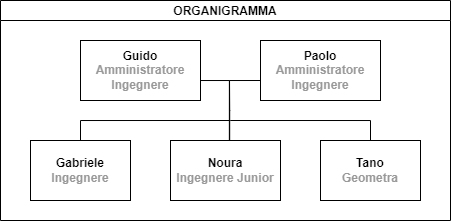
\includegraphics[scale=0.6]{../Img/Diagrams/Organigramma}
	\end{figure}	
	\chapter{Raccolta ed Analisi dei Requisiti}
	
	Il capitolo si suddivide in "Raccolta dei Requisiti" e "Analisi dei Requisiti".
        Nella prima parte abbiamo documentato e trascritto le interviste svolte in maniera formale a tecnici e titolari dello Studio.
        Nella seconda parte, invece, abbiamo analizzato il contenuto delle interviste e dei documenti traendo poi le conclusioni finali per quanto riguarda i Requisiti.
	
	\section{Raccolta dei Requisiti}
	
	Questa sezione è divisa in "Interviste" e "Documenti".
        Nella prima troverete la trascrizione delle interviste svolte in maniera formale con tecnici e titolari dello Studio.
        Nella seconda una discussione e illustrazione della documentazione che ci è stata fornita dallo Studio.
	
	\subsection{Interviste}
	\textbf{Nota:} nelle trascrizioni delle interviste abbiamo usato le seguenti notazioni:
	\begin{itemize}
		\item \textbf{B:} indica che l'interlocutore è Began Bajrami;
		\item \textbf{R:} indica che l'interlocutore è Rahmi El Mechri;
		\item \textbf{RnB:} indica quei momenti in cui entrambi gli intervistatori hanno espresso lo stesso concetto con parole diverse.
                    Per evitare ripetizioni, abbiamo sintetizzato in questa maniera;
		\item \textbf{[n.d.r. $<$contenuto$>$ ]:} nota del redattore.
	\end{itemize}
	
	Le seguenti interviste sono state riadattate per una lettura più facile, poiché il parlato risulta spesso molto più confuso da scritto,
        cercando comunque di mantenere la personalità degli interlocutori.
	
	\subsubsection{Intervista a Tecnico(Gabriele)}
	
	Di seguito è trascritta la prima intervista, effettuata in loco la mattina del 12 Novembre 2021 a \textbf{Gabriele}, un tecnico dello Studio.
        Durante il colloquio interverrà anche Guido, uno dei due titolari dello studio, che era presente ma non disponibile per una intervista diretta.
	
	\begin{itemize}
		\item\textbf{RnB}\textbf{:} Sappiamo già, in realtà a grandi linee, di cosa si occupa lo studio, però ci teniamo comunque a cominciare
                    l'intervista chiedendovi più nello specifico "di cosa vi occupate"?
		\item\textbf{Gabriele}\textbf{:} Allora, Progettazione urbanistica, pratiche comunali catastali varie; ci occupiamo di "direzione lavori"...
		\item\textbf{RnB}\textbf{:} Cosa intendi con "direzione lavori"?
		\item\textbf{Gabriele}\textbf{:} In pratica, la persona che si occupa di seguire le varie lavorazioni che vengono fatte in cantiere ma non in impresa...
                    un controllore super partes, diciamo.
                    Poi facciamo pratiche di antincendio, come "Certificati Prevenzione Incendi", quindi analisi dei fattori di rischio che facciamo per 
                    autorimesse, aziende, e così via.
		\item\textbf{R}\textbf{:}Quindi intendi controlli della struttura e cose di questo genere?
		\item\textbf{Gabriele}\textbf{:} Più che controlli diciamo implementazione e controllo di strutture esistenti. Ad esempio un amministratore ci potrebbe dire:
                    "guarda io devo verificare se questa autorimessa è a norma". Mentre per quanto riguarda l'antincendio è anche più ampio perché può andare sia sul "nuovo"
                    che sul "vecchio". Noi l'anno scorso [n.d.r. nel 2020] abbiamo seguito soprattutto il cambio sul DM del 25 Gennaio 2019, se non sbaglio,
                    che cambiava l'altezza da dove veniva preso l'antincendio.
                    E questa è la parte, diciamo, "antincendio".
                    Paolo ha il timbro iscritto al ministero per lavori riguardanti l'antincendio. Per avere l'attestato, per fare questa cosa qui,
                    serve un corso molto lungo e devi quindi essere certificato. Guido invece ce l'ha per l'acustica, quindi per fare certificati acustici che servono spesso
                    e volentieri sulle pratiche quando vengono modificate bucature o cose del genere.
		\item\textbf{R}\textbf{:} Bucature?
		\item\textbf{Gabriele}\textbf{:} Bucature, quindi le finestre. Se vengono modificate le dimensioni delle finestre o le attività che vengono fatte all'interno
                    di uno stabile, devi fare un certificato dal punto di vista acustico in modo che non dia fastidio al vicinato.
		\item\textbf{R}\textbf{:} Ok perfetto. Poi ho visto che vi occupate anche tanto di ristrutturazioni a causa del 110\% quest'anno.
		\item\textbf{Gabriele}\textbf{:} Le ristrutturazioni sono alla base della progettazione urbanistica, che comprende "nuovo" e "vecchio".
                    Il "nuovo" è ovviamente più raro, però abbiamo lavorato anche a progetti di questo tipo. Ma, come dicevo, il nuovo è solo un 10\%, 15\% dei lavori di
                    progettazione urbanistica, la maggior parte è "vecchio".
		\item\textbf{R}\textbf{:} Bene, è molto importante per noi sapere quali sono i lavori che svolgete più frequentemente.
		\item\textbf{B}\textbf{:} Giusto un chiarimento: con \textbf{ "vecchio" } cosa si intende? Progetti già esistenti?
		\item\textbf{Gabriele}\textbf{:} "vecchio" significa lavori di ristrutturazione o modifiche di strutture già presenti, ed è
                    \textbf{ la maggior parte del nostro lavoro}, poiché nuove costruzioni sono molto rare.
                    Paolo, ma anche Guido, fanno anche pratiche di tribunale, quindi CTU (Consulente Tecnico Unico) o CTP (Consulente Tecnico di Parte), ma soprattutto CTU,
                    che sono quelle pratiche in cui tu ti metti a disposizione di un tribunale che ha un contenzioso, ovvero una causa che deve valutare, e se serve mette di
                    mezzo un tecnico che fa una consulenza "super partes". Nelle CTP invece sei il tecnico di una delle due parti. Devi comunque essere oggettivo,
                    però cerchi di fare i favori del tuo cliente. Facciamo anche perizie di stima.
		\item\textbf{B}\textbf{:} Con \textbf{perizia} cosa si intende? 
		\item\textbf{Gabriele}\textbf{:} Una perizia è un lavoro nel quale devi dare un parere tecnico oggettivo su un qualcosa.
                    Prendiamo il caso in cui ci sia stato un danno: un tecnico ti fa una relazione su quanto è successo, e questo è un tipo di perizia.
                    Oppure, un'altra situazione può essere quando un cliente ci chiede: "quanto vale quel capannone?" e quindi tu devi fare una analisi oggettiva tramite 
                    l'unione di vari dati per capirne il valore di costruzione, dati come: il luogo, cosa ci puoi fare, cosa c'è intorno, l'usura, e molti altri fattori.
		\item\textbf{RnB}\textbf{:} Notiamo che fate molti tipi di lavori diversi, c'è dell'altro?
		\item\textbf{Gabriele}\textbf{:} L'ultima cosa, facciamo anche industria 4.0, ma puoi metterla anche sotto perizia fondamentalmente.
		\item\textbf{B}\textbf{:} Con industria 4.0 a cosa ti riferisci?
		\item\textbf{Gabriele}\textbf{:} Industria 4.0 è, diciamo, un procedimento che c'è ultimamente dove, in pratica, se un macchinario segue alcune specifiche
                    di interconnessione, modernità e controllo a distanza in una rete ha grossi sgravi fiscali. Facciamo un esempio: uno degli ultimi era un tornio
                    controllabile a distanza tramite applicazione, che era all'interno dell'azienda interconnesso tramite una rete, che era "intelligente"; questo ha enormi
                    sgravi fiscali.
		\item\textbf{B}\textbf{:} In azienda c'è qualcuno effettivamente che lavora solo con i dati? Ci lavorate tutti oppure c'è una sorta di divisione?
		\item\textbf{Gabriele}\textbf{:} Tutti. Infatti siamo tutti collegati al server collocato davanti all'antibagno, e abbiamo anche un tecnico informatico che
                    si occupa dei guasti.
		\item\textbf{RnB}\textbf{:} Hai qualche problema o trovi difficoltà con l'attuale gestione dei dati? C'è qualcosa che vorresti risolvere? 
		\item\textbf{Gabriele}\textbf{:} Allora, il problema più grosso che abbiamo noi è che: poiché persone diverse lavorano in modo diverso, quando tu vai a 
                    lavorare su file, cartelle e pratiche gestiti da altri, non tutti ragionano allo stesso modo e quindi è difficile recuperare alcune informazioni. 
                    Velocemente ovviamente, poi cercando si trova tutto.
		\item\textbf{B}\textbf{:} In realtà è molto importante come osservazione perché i database mirano, tra le altre cose, a risolvere questo problema, perché
                    standardizzano questi dati rendendo la loro gestione più facile.
		\item\textbf{R}\textbf{:} Come sono divisi i lavori tra di voi?
		\item\textbf{Gabriele}\textbf{:} Fondamentalmente ognuno ha alcune cose che fa in modo specifico. Ad esempio la parte di acustica la fa Guido, la parte di
                    Antincendio la imposta Paolo ma spesso e volentieri la facciamo io e Tano. Però di solito è un "tutti fanno tutto". Ovviamente Paolo e Guido hanno più
                    esperienza e più conoscenze e quindi il lavoro arriva a loro e viene smistato nella nostra rete.
		\item\textbf{RnB}\textbf{:} Ok, perfetto, grazie.
		\item\textbf{Gabriele}\textbf{:} Nel nostro ambito ci sono tante cose ma sono tutte non troppo distanti, ad esempio noi "Impiantistica" non la facciamo e
                    quindi quando arriva qualcosa di quel genere la passiamo a chi di dovere. Ad esempio nei lavori di ristrutturazione legati al "Superbonus 110\%"
                    collaboriamo con una società di termotecnici.
		\item\textbf{R}\textbf{:} Quindi voi state lavorando anche con società terze perciò? 
		\item\textbf{Gabriele}\textbf{:} In realtà noi tutto quello che non facciamo lo diamo da fare a terzi. Quindi quando ci viene affidato un incarico che non è
                    nel nostro dominio di lavoro, giriamo la richiesta ad una società terza, ed alcune volte collaboriamo per lavorare sugli stessi progetti, spesso con più
                    di una, ad esempio la parte di impiantistica viene affidata ad una società, mentre l'analisi urbanistica del luogo è stata affidata ad un'altra.
                    Ovviamente in tutto ciò il cliente deve essere d'accordo. L'onorario ovviamente verrà poi diviso tra le varie società.
		\item\textbf{R}\textbf{:}Voi non avete una base di dati digitale, ma avete praticamente tutto cartaceo, no? A parte,  ovviamente, quello che ci avete mostrato.
		\item\textbf{Gabriele}\textbf{:} Qua dietro c'è l'archivio [n.d.r. cartaceo], però è datato. Da diversi anni molte delle pratiche sono digitali, ma non sono
                    gestite, sono sparse nelle cartelle. Una implementazione un pò più importante che abbiamo fatto recentemente è un server condiviso con un'altra società,
                    ma quello è il limite. Come vedete ancora di carta ce n'è tanta. Anche perché, ad esempio, questo è il sito del comune di Ancona.
		\\
	\end{itemize}
	
	Gabriele ci ha mostrato il portale del comune di Ancona e quello di Montefano. Ci ha mostrato che il portale funge da raccoglitore, dove inseriscono documentazioni
        relative al comune. I portali condividono la stessa infrastruttura, infatti per accedervi utilizzano le stesse credenziali. Inoltre, Gabriele ci mostra un file Excel
        con una tabella nella quale salvano informazioni relative ai progetti riguardanti il "Superbonus 110\%".
	\\
	\begin{itemize}		
		\item\textbf{R}\textbf{:} Ci sono particolari richieste che potrebbero semplificare il tuo lavoro che ti piacerebbe vedere implementate nel database?
		\item\textbf{Gabriele}\textbf{:} Una cosa ci sarebbe: quando si realizza un cantiere c'è da fare il PSC (Piano Sicurezza e Coordinamento) se ci sono tante
                    ditte che lavorano nello stesso cantiere, ovvero un documento che coordina gli orari di lavoro delle diverse ditte; avere nel database le varie ditte
                    senza doverle andare sempre a cercare farebbe comodo.
		    Un'altra informazione che sarebbe utile avere nel database sono ad esempio le scadenze dei CPI (Certificato Prevenzione Incendi).
		\item\textbf{RnB}\textbf{:} Poiché il vostro è un lavoro nel quale le normative sono estremamente importanti, ci sono dati riguardanti questo aspetto che ti
                    piacerebbe salvare per semplificare le vostre operazioni?
		\item\textbf{Gabriele}\textbf{:} Diciamo di no, poiché i documenti sono tutti estremamente diversi tra loro e spesso sono documenti realizzati ad hoc per la
                    situazione, quindi difficilmente standardizzabili.
		\item\textbf{B}\textbf{:} C'è un'organizzazione per i dati che salvate?
		\item\textbf{Gabriele}\textbf{:} Quando fai un lavoro devi fare una cartella. Dentro la cartella devi almeno dividere quello che stai facendo.
		\item\textbf{B}\textbf{:} Quindi non c'è una standardizzazione nella gestione delle varie cartelle, ma ti piacerebbe implementarne una?
		\item\textbf{Gabriele}\textbf{:} Mi piacerebbe standardizzare questo aspetto, ma è impossibile.
		\item\textbf{B}\textbf{:} Perché?
		\item\textbf{Gabriele}\textbf{:} Perché ognuno lavora con la propria testa, sarebbe molto difficile anche perché molte volte facciamo tutto di fretta.
		\item\textbf{B}\textbf{:} A parte i dati che tenete nella cartella, ci sono anche dati cartacei, giusto? Il contenuto di questi archivi è "identico" a
                    quello che si trova nel server oppure sono proprio dati differenti?
		\item\textbf{Gabriele}\textbf{:} Ultimamente stiamo digitalizzando, prima raccoglievamo i vari documenti all'interno di un raccoglitore, ora invece li
                    scannerizziamo e li mettiamo nel server.
                \\
	\end{itemize}
	A questo punto Gabriele ci porta a vedere l'archivio dei dati cartacei, ormai rimasto per mantenere una integrità storica dei dati.
        \\
	\begin{itemize}
		\item\textbf{B}\textbf{:} Questi raccoglitori sono organizzati in qualche modo?
		\item\textbf{Gabriele}\textbf{:} Ci sono dei foglietti attaccati agli scaffali davanti ad alcune cartelle, in linea di massima sono un sommario di quello
                    che c'è nelle cartelle coperte dal foglietto. Non si va nel dettaglio, è molto generico. In conclusione: se stai cercando qualcosa, devi sapere dove si
                    trova, altrimenti è difficile riuscire a trovare quello che si cerca.
		\item\textbf{B}\textbf{:} Quindi qua sostanzialmente si trova lo stesso tipo di dati che in questo momento digitalizzate, però in forma cartacea, no?
		\item\textbf{Gabriele}\textbf{:} Si, per un 90\% è così.
		\item\textbf{B}\textbf{:} Una cosa di cui vorrei essere molto sicuro è che qua non ci siano dati particolari che in digitale non esistono già, cioè che
                    vengono mantenuti esclusivamente in forma cartacea.
		\item\textbf{Gabriele}\textbf{:} Le robe molto vecchia magari qualcosa può essere, però per il resto no.
                \\
	\end{itemize}
	Dopo la breve visita all'archivio, contenente solo dati di rilevanza storica per lo Studio, poiché ormai lavorano solo in digitale, torniamo in ufficio
        \\
	\begin{itemize}
		\item\textbf{B}\textbf{:} In azienda è prevista una sorta di controllo, revisione dei dati per verificare se effettivamente il lavoro svolto è coerente o
                    che non ci siano sbagli? 
		\item\textbf{Gabriele}\textbf{:} Noi ci controlliamo tra di noi.
		\item\textbf{B}\textbf{:} Quindi non c'è un controllo specifico, ma avviene comunque perché ognuno mentre ci lavora ricontrolla un pò quello che è stato
                    fatto dagli altri.
		\item\textbf{Gabriele}\textbf{:} Esattamente. Spesso Paolo e Guido, avendo più esperienza, seguono insieme a noi le pratiche più complicate per evitare
                    errori, ma molte volte lavoriamo in modo autonomo.
		\item\textbf{R}\textbf{:} A livello di gestione dati, come dovete tenerli? Come vi comportate con essi? Ci sono normative su come mantenere, organizzare e
                    distribuire i dati?
		\item\textbf{Gabriele}\textbf{:} Ci sono solo le normative standard sulla privacy e poco più.
		\item\textbf{B}\textbf{:} Niente di obbligatorio da mantenere del cliente?
		\item\textbf{Gabriele}\textbf{:} Questo non lo so, chiedete magari a Paolo o Guido.
                \\
	\end{itemize}
	Poiché Gabriele è un tecnico non conosce bene questo aspetto, verrà approfondito nell'intervista a Paolo, uno dei due titolari.
        \\
	\begin{itemize}
		\item\textbf{R}\textbf{:} Ci sono altri tipi di dati che vi piacerebbe gestire meglio?
		\item\textbf{Gabriele}\textbf{:} Le fatture, che al momento gestiamo con dei file Excel. 
                \\
	\end{itemize}
	Ci mostra un file Excel dove c'è una tabella che contiene informazioni relative alle fatture.
        \\
	\begin{itemize}
		\item\textbf{B}\textbf{:} C'è una struttura particolare in questo elenco di fatture o no?
		\item\textbf{Gabriele}\textbf{:} Ti faccio vedere la mia, io ho un mio elenco di fatture...
		\item\textbf{B}\textbf{:} Quindi questo è il tuo elenco personale? Ognuno ha una propria scheda?
		\item\textbf{Gabriele}\textbf{:} Si questo è mio. In cui c'è la data di immissione, se è stato pagato, ed altre informazioni di questo tipo.
		\item\textbf{B}\textbf{:} Le tabelle che avete però sono standardizzate giusto?
		\item\textbf{Gabriele}\textbf{:} Una fattura di Paolo, ad esempio, è fatta con Excel, mentre la mia con Word, ma se vai a vedere le mie ho qualche dato in
                    meno rispetto alla sua tabella.
		\item\textbf{R}\textbf{:} Noi dobbiamo fare uno studio sul tipo di operazioni che fate più frequentemente e sulla mole di dati divisa per tipo, dunque ti
                    chiedo: quali sono i dati a cui accedi più frequentemente? Quali sono le operazioni che svolgi in una tua giornata tipo?
		\item\textbf{Gabriele}\textbf{:} Dipende, questa domanda non ha risposta. Dipende molto da cosa devo fare giorno per giorno. Ci sono dei giorni in cui il
                    computer non lo apro quasi mai praticamente.
		\item\textbf{Guido}\textbf{:} Dipende dalla gestione dell'attività. Se fai progettazione stai qui. Se fai sopralluoghi ovviamente vai là.
		\item\textbf{R}\textbf{:} Per fare invece una stima dei dati, quanti progetti fate all'anno? Immagino che per ogni progetto ci sia una fattura, giusto?
		\item\textbf{Gabriele}\textbf{:} Dipende. Ci sono più progetti che fatture.
		\item\textbf{Guido}\textbf{:} Un centinaio di progetti all'anno. Alcuni sono anche preventivi.
		\item\textbf{RnB}\textbf{:} Bene, grazie per averci dedicato il tuo tempo.
	\end{itemize}
	\newpage
	\subsubsection{Intervista a Tecnico(Noura)}
	\begin{itemize}
		\item \textbf{R:} Parliamo dei progetti. Analizzando l'intervista effettuata a Gabriele e la scheda flusso dei lavori inerenti al superbonus 110\%, ho
                    identificato le seguenti informazioni che potrebbero essere comuni ad ogni progetto: cliente che richiede il progetto, proprietario della struttura,
                    locazione della struttura, tipo di lavoro, la data di inizio e fine per l'accesso agli atti, per i sopralluoghi e  per il computo. Potresti confermarmi se effettivamente queste informazioni sono comuni a tutti i progetti, e se ci sono ulteriori informazioni da
                    riportare? Potresti descrivermi il significato di queste date?
		\item \textbf{Noura:} Le informazioni che hai elencato sono corrette. L'accesso agli atti è il procedimento durante il quale si ritirano gli atti depositati
                    in comune relativi alla struttura, ovvero i documenti riguardanti il progetto iniziale, gli oneri pagati, eventuali varianti al progetto, modifiche
                    successive, e lavori che sono stati depositati. Quest'ultima parte è importante, poiché potrebbero essere stati fatti dei lavori sulla struttura che non
                    sono stati depositati in comune; questo viene verificato con i sopralluoghi, perciò, prima di cominciarli, si portano gli atti in ufficio e li analizziamo,
                    controllando la pianta della struttura, e quindi poi fissiamo la data del sopralluogo. Se il sopralluogo coincide con gli atti si procede con la proposta
                    al cliente, se invece le informazioni riportate negli atti non coincidono con la realtà ci sono delle modifiche da fare, quindi di procede con delle
                    SCIA (Segnalazione Comunicazione Inizio Lavori) in Sanatoria o delle CILAS(Comunicazione Inizio Lavori Asseveramento Semplificata), ovvero dei documenti
                    che attestano l'inizio dei lavori.
		\item \textbf{R:} (Interrompo) Si fa o uno o l'altro, ho capito bene?
		\item \textbf{Noura:} Esattamente, la CILAS nasce come variante più "snella" della SCIA, ma in alcuni casi il comune potrebbe richiedere una SCIA poiché più
                    completa.
		\item \textbf{R:} Bene, cosa accade dopo questo passaggio?
		\item \textbf{Noura:} A questo punto c'è l'Accatastamento, ovvero il deposito al catasto delle modifiche effettuate sulla struttura, poiché anche l'agenzia
                    delle entrate ne tiene traccia.
		\item \textbf{R:} E questo passaggio avviene sempre dopo la CILAS o la SCIA?
		\item \textbf{Noura:} Ci sono dei casi in cui il cliente ha depositato le modifiche al catasto, e quindi ha già effettuato l'accatastamento, ma non le ha
                    depositato e in comune.
		\item \textbf{R:} A questo punto che succede?
		\item \textbf{Noura:} A questo punto si fa la proposta dei costi al cliente. Questi ultimi passaggi avvengono solo se ci sono delle modifiche non a norma,
                    perciò al cliente viene addebitata una somma maggiore di denaro quando si farà la proposta. In alcuni casi infatti questo procedimento può avere dei costi
                    tali da superare il budget del cliente, quindi lo si comunica al cliente, ed eventualmente si chiude il progetto, o in altri casi invece che utilizzare il
                    superbonus 110\%, che riguarda anche gli interni, si decide di lavorare solo sugli esterni con il superbonus 90\%, che richiede che sia sistemato solo
                    l'esterno della struttura.
		\item \textbf{R:} A proposito degli sgravi fiscali, abbiamo pensato potesse essere utile sapere quali sgravi fiscali sono stati applicati al progetto, che
                    ne pensi?
		\item \textbf{Noura:} Credo che sia una buona idea.
		\item \textbf{R:} Nell'intervista con Gabriele ci è stato spiegato che lo studio partecipa a lavori di consulenza come CTU e CTP, nei quali le informazioni
                    appena elencate non sono necessarie, data la natura diversa di quest'ultimi. E' errato non considerarli come dei progetti?
		\item \textbf{Noura:} No è coretto, non sono dei progetti poiché con le CTU e le CTP non si progetta, bensì si da un consiglio al tribunale.
		\item \textbf{R:} Che informazioni bisogna conoscere riguardo le CTU e le CTP?
		\item \textbf{Noura:} Bisogna salvare chi è stato nominato dal tribunale, gli avvocati impegnati nella questione, quindi il loro nome e i loro contatti, e
                    qual è l'oggetto di contesto: a seconda di quest'ultimo l'ingegnere nominato dall'albo può decidere se rifiutare o meno, valutando le proprie competenze,
                    poiché il tribunale pesca un ingegnere direttamente dalla lista degli ingegneri iscritti all'albo, senza conoscere quali sono le sue competenze, spetta
                    all'ingegnere decidere se accettare o meno, valutando se ha le competenze adatte, ovvero i certificati necessari.
		\item \textbf{R:} Me ne ha parlato anche Gabriele, ritieni che sarebbe utile sapere per ogni tecnico dello studio le certificazioni che possiede?
		\item \textbf{Noura:} Si, sarebbe molto utile.
		\item \textbf{R:} Per comprendere ancora meglio la differenza tra i progetti e gli altri tipi di lavoro, potresti descrivermi i processi interni che avvengono
                    a partire dalla richiesta del cliente per quanto riguarda i progetti?
		\item \textbf{Noura:} Il cliente chiama Paolo...
		\item \textbf{R:} Che si intende per cliente? Coincide sempre con il proprietario della struttura?
		\item \textbf{Noura:} In genere cliente e proprietario coincidono, ma ci sono casi in cui le strutture hanno più co-proprietari, e dobbiamo avere i dati di
                    ognuno di loro. Il cliente può essere un'azienda o una persona. Le aziende di solito ci chiamano quando vogliono aprire delle nuove sedi, o quando
                    devono fare dei lavori di ristrutturazione nei loro plessi, quindi ci chiamano per effettuare una valutazione per capire come sarà il progetto, e per 
                    capire quali certificazioni serviranno. Ad esempio per un magazzino che contiene sostanze infiammabili servirà un CPI(Certificato Prevenzione Incendi). 
                    Dobbiamo capire quali sono le esigenze del cliente per capire bene i certificati necessari. Se è una struttura da costruire che non esiste si procede con 
                    la proposta iniziale. Se si lavora su una struttura preesistente te, si controlla che sia a norma ai fini del progetto, ed eventualmente si procede con il
                    CILAS o SCIA in Sanatoria, e poi con l'accatastamento. Ad esempio nei casi di migliorie si deposita direttamente la modifica poiché ai fini del progetto 
                    non importa che eventuali modifiche siano a norma o meno; in altri casi invece è importante fare uno studio della struttura, poiché ci sono dei requisiti 
                    da rispettare, come quelli igenico-sanitari. Altri studi prevedono una valutazione del terreno, e questo comporta dei costi per chiamare il geo-tecnico 
                    che effettua un carotaggio, che serviranno anche a capire che tipo di fondazioni utilizzare. A questo punto si redige un onorario del tecnico, poiché anche
                    se il cliente decidesse di non accettare la proposta, ci sono dei costi per la valutazione effettuata da affrontare. Se il cliente non accetta la proposta
                    si ferma il progetto. Se il cliente accetta si fa uno studio sulle imprese da chiamare per collaborare, e capire quali figure coinvolgere, come un 
                    impiantista. A questo punto si definisce il progetto definitivo, e quindi il cliente può decidere se approvare il progetto, o richiedere delle modifiche, 
                    ad esempio richiedere che in un lato della casa non ci siano finestre. Se cosi fosse si modifica il progetto e lo si ripropone. Prima di proporre il 
                    progetto definitivo si effettua il computo metrico, che definisce in modo preciso i costi dei lavori e dei materiali, poiché quello prima della proposta 
                    iniziale è un computo di massima, che stima i costi. Una volta approvato dal cliente si fa un controllo delle certificazioni, e poi si deposita il progetto
                    in comune. Una volta approvato dal comune si contattano le imprese per iniziare i lavori. Le imprese con cui si collabora variano di volta in volta, 
                    poiché potrebbero essere occupate per altri progetti.
		\item \textbf{R:} Che informazioni vi servono sulle imprese?
		\item \textbf{Noura:} Ci serve sapere il nome ovviamente, l'indirizzo dov'è collocata l'impresa, e i 
                    contatti come email e telefono. Ti manderò un documento dove sono presenti le varie informazioni che ci servono.
		\item \textbf{R:} Perfetto grazie. A questo punto come si procede?
		\item \textbf{Noura:} Si avverte l'ASL dell'inizio dei lavori, e comincia la parte di cantiere.
		\item \textbf{R:} Mi ha detto Gabriele che vi occupate anche del PSC(Piano Sicurezza e Coordinamento)?
		\item \textbf{Noura:} Esattamente, è un documento che serve per coordinare le lavorazioni principalmente per questione di sicurezza; due ditte non possono 
                    lavorare sullo stesso punto, inoltre alcune lavorazioni sono più pericolose o prendono più tempo, quindi il PSC serve anche per gestire le tempistiche, 
                    considerando anche eventuali problemi di maltempo.
		\item \textbf{R:} Iniziato il cantiere vi occupate voi della parte di Direzione Lavoro?
		\item \textbf{Noura:} Dipende, se ci nominiamo come Direttori del Lavoro allora ci occupiamo anche della parte di direzione, dove si controlla che i lavori 
                    avvengano come prestabilito.
		\item \textbf{R:} Serve una certificazione per farlo?
		\item \textbf{Noura:} No, basta essere iscritti all'albo.
		\item \textbf{R:} Ok. A questo punto c'è altro?
		\item \textbf{Noura:} C'è lo stato di avanzamento lavori, perché se il cliente non mi paga ogni tot potrei anche fermarmi coi lavori. Una volta completato 
                    il lavoro si fa un sopralluogo per verificare che quello che il progetto depositato sia stato rispettato, c'è il collaudo e il controllo agibilità. 
                    Infine si comunica al comune la fine dei lavori.
		\item \textbf{R:} Il processo per le CTU e le CTP invece?
		\item \textbf{Noura:} Il giudice al tribunale nomina un tecnico iscritto all'albo da almeno dieci anni, e questo tecnico deve fare una valutazione in una 
                    controversia. Il tecnico fa un sopralluogo insieme a uno o entrambi gli avvocati delle parti, e consegna la documentazione.
	\end{itemize}
	\newpage
	\subsubsection{Intervista a Titolare(Paolo)}
	\begin{itemize}
		\item \textbf{RnB:}Analizzando il vostro lavoro e i vostri documenti abbiamo già ipotizzato quale potrebbero essere i dati riguardanti i clienti che dovete 
                    conoscere, volevamo quindi sapere cosa ne pensi? (Mostriamo i requisiti sui clienti ottenuti fino ad'ora)
		\item \textbf{Paolo:} Ci sono 3 tipi di clienti: i privati, le società e il tribunale. La vostra analisi va bene per i privati, ma quando lavoriamo con le 
                    società interagiamo con chi ci contatta. Quindi anche se i dati, nonostante i cambiamenti che una società può fare, sono sempre gli stessi, il contatto 
                    che abbiamo cambia continuamente. Ci è capitato di lavorare con una società X nella quale avevamo come contatto questo amministratore delegato, che ora ha
                    cambiato, e lavora con una società Y, ed ora entrambe sono nostre clienti. Per quanto riguarda i tribunali abbiamo contatti con dei giudici, con cui 
                    lavoriamo per perizie di stime e consulenze. Esiste in realtà anche un quarto tipo di clientela, ovvero i condomini, collaboriamo con 32 amministratori 
                    nel comune di Ancona e provincia. Le prestazioni che forniamo ai vari clienti sono di diverso tipo, ma si dividono principalmente in progettazioni e 
                    consulenze. Le consulenze posso essere antincendio, acustiche, energetiche, catastali e perizie. Delle consulenze antincendio me ne occupo io poiché ho 
                    fatto un corso di 120 ore a riguardo, mentre alle acustiche ci pensa Guido che ha fatto anche lui un corso di 120 ore ma relativo all'acustica. Di 
                    consulenze energetiche ne facciamo poche, mentre delle catastali, cioè verifiche ed aggiornamenti catastali, ce ne occupiamo tutti. Le perizie di stima 
                    sono invece delle valutazioni del valore di strutture. I privati ci chiedono ristrutturazioni e costruzioni di case nuove. Con le società invece si 
                    tratta di progetti più importanti, dove si fanno riunioni con l'amministratore delegato, poiché parliamo di centinaia di migliaia di euro. Uno dei nostri 
                    problemi è che il nostro sistema di archiviazione è piuttosto grezzo, io mi trovo bene col mio modo di lavorare, ma chiaramente quando si fa teamwork 
                    diventa un problema poiché ognuno ha il proprio modo per organizzare i dati. 
		\item \textbf{RnB:} Quali informazioni cambiano a seconda del tipo cliente?
		\item \textbf{Paolo:} Tanto per cominciare quando si parla di privati o condomini abbiamo bisogno di un codice fiscale, mentre per le aziende la loro partita IVA. Ci sono anche casi in cui ci servono entrambe.
		\item \textbf{B:} Avresti dei documenti dove possiamo vedere quali sono i dati necessari da conoscere sui clienti?
		\item \textbf{Paolo:} Noi non salviamo direttamente i dati dei clienti, arriviamo a conoscerli un po' alla volta poiché dobbiamo compilare alcuni moduli che 
                    li richiedono, volete vederli?
		\item \textbf{RnB:} Si, grazie.
		\\
	\end{itemize}
	Paolo ci mostra alcuni documenti riguardanti dei progetti su cui stanno lavorando, in particolare ci mostra i dati riguardanti i clienti che debbono essere inseriti per poter avviare una procura a loro nome, sia nel caso che si tratti di privati, che nel caso di aziende; ci viene consegnato un modulo della procura cartaceo.
	\\
	\begin{itemize}
		\item \textbf{B:} Che normative seguite per quanto riguarda la privacy?
		\item \textbf{Paolo:} La legge 231 e il GDPR.
		\item \textbf{R:} Abbiamo raccolto quelle che pensiamo siamo le informazioni necessarie per quanto riguarda i progetti, cosa ne pensi? Ci potresti dire se 
                    potrebbe essere utile gestire altro?
		\item \textbf{Paolo:} Le informazioni vanno bene però non tutti i progetti prevedono l'accesso agli atti e i sopralluoghi.
		\\
	\end{itemize}
	Paolo ci mostra Stimatrix, una piattaforma che permette di conoscere le informazioni catastali delle strutture.
	\\
	\begin{itemize}
		\item\textbf{Paolo:} Potrebbe essere utile conoscere l'identificativo catastale, ovvero per la struttura conoscere Comune, foglio, particella e subalterno.
	\end{itemize}
	\newpage
	\subsection{Documenti}
	
	Durante le interviste abbiamo avuto modo di vedere in presenza documenti di vario genere, sia cartacei che digitali. Inoltre, i tecnici e i titolari si sono mostrati
        disponibili a fornirci di tutta la documentazione necessaria anche al di fuori degli orari di lavoro, comunicando tramite email. In questa sezione mostriamo, con il
        dovuto rispetto della privacy, tutti i documenti che ci sono stati utili alla analisi dei requisiti.
	\subsubsection{Tabella Progetti "Superbonus 110\%"}
	
	Poiché lo Studio ha molto a che fare con le 110\%, usa un file Excel che tiene conto dei dati relativi alla questione. Di seguito una descrizione del contenuto del file:
        \begin{center}
		\begin{longtable}{|l|p{10cm}|}
			\hline
			\textbf{Proprietario} & Nome e cognome del proprietario della struttura\\
			\hline
			\textbf{Dati} & Codice fiscale, data di nascita, luogo di nascita, residenza, numero di telefono ed email del cliente del proprietario della struttura.\\
			\hline
			\textbf{Valutazione preliminare eseguita} & Lista degli interventi possibile post studio di fattibilità.\\
			\hline
			\textbf{Incarico inviato} & Data invio proposta al cliente.\\
			\hline
			\textbf{Incarico firmato} & Data firma del cliente.\\
			\hline
			\textbf{Interventi} & Lista interventi che si effettueranno.  \\
			\hline
			\textbf{Accesso agli atti inviato} & Data richiesta accesso agli atti della struttura.\\
			\hline
			\textbf{Accesso agli atti eseguito} &  Data in cui termina la parte di accesso agli atti.\\
			\hline
			\textbf{Sopralluoghi iniziati} & Data inizio sopralluoghi.\\
			\hline
			\textbf{Sopralluoghi terminati} & Data fine sopralluoghi. \\
			\hline
			\textbf{Invio a sezione termotecnica} & Data inizio analisi termotecnica da parte dell'azienda collaboratrice competente. \\
			\hline
			\textbf{Fine analisi termotecnica} & Data fine analisi termotecnica da parte dell'azienda collaboratrice competente.\\
			\hline
			\textbf{Valutazione interventi} & Valutazione sugli interventi possibili post analisi termotecnica.\\
			\hline
			\textbf{Inizio computo} & Data inizio compilazione computo per definire il costo degli interventi.\\
			\hline
			\textbf{Fine computo} & Data fine compilazione computo.\\
			\hline
			\textbf{Fase al DD/MM/AAAA} & Descrizione dello stato in cui si trova il progetto in data DD/MM/AA. \\
			\hline	
		\end{longtable}
	\end{center}
	\newpage
	\subsubsection{Tabella Fatture}
	
	Di seguito viene rappresentata la tabella delle fatture aziendali. Attualmente, lo Studio usa un foglio di calcolo Excel dove organizza questi dati.
	\begin{center}
		\begin{longtable}{|l|p{10cm}|}
			
			\hline
			\textbf{Numero Fattura} & Il numero (identificativo) della fattura. \\
			\hline
			\textbf{Cliente} & Nome e cognome del cliente.\\
			\hline
			\textbf{Data emissione pre-fattura} & Data in cui è avvenuta l'emissione della pre-fattura.\\
			\hline
			\textbf{Data emissione fattura} & Data in cui è avvenuta l'emissione della fattura.\\
			\hline
			\textbf{Data incasso} & Data in cui è avvenuto l'incasso della fattura.\\
			\hline
			\textbf{Modalità} & Madalità di pagamento (presente solo se è avvenuto l'incasso).\\
			\hline
			\textbf{Tipo} & Tipologia di fattura.\\
			\hline 
			\textbf{Imponibile} & Valore su cui viene applicata l'aliquota per calcolare l'imposta.\\
			\hline
			\textbf{CNPAIA (4\%)} & Contributo Inarcassa 4\%.\\
			\hline
			\textbf{IVA (22\%)} &  Imposta sul valore aggiunto ordinaria.\\
			\hline
			\textbf{Ritenuta acconto} & Quota anticipo pagata dal cliente.\\
			\hline
			\textbf{Costi esenti IVA} & Costi che non concorrono alla formazione della base imponibile.\\
			\hline
			\textbf{Totale fattura} & Totale somma che verrà versata.\\
			\hline
			\textbf{Rit. banca su ristrutturazioni} & Quota ritenuta dalla banca in caso di lavoro di ristrutturazione.\\
			\hline
			\textbf{Totale incassato} & Somma che lo studio riceve.\\
			\hline
		\end{longtable}
	\end{center}
	\newpage
	\subsubsection{Procura}
	Versione digitale della Procura consegnataci durante l'intervista con Paolo.
		\begin{figure}[H]
			\centering
			
\includegraphics[scale=0.8]{../Img/Documents/Procura/Procura-1.png}
		\end{figure}
		\begin{figure}[H]
			\centering
			
\includegraphics[scale=0.8]{../Img/Documents/Procura/Procura-2.png}
		\end{figure}
	\newpage
	\subsubsection{CILA}
	Documento di una CILA(Comunicazione Inizio Lavori Asseverata) utilizzato per raccogliere informazioni sui dati necessari.
		\begin{figure}[H]
			\centering
			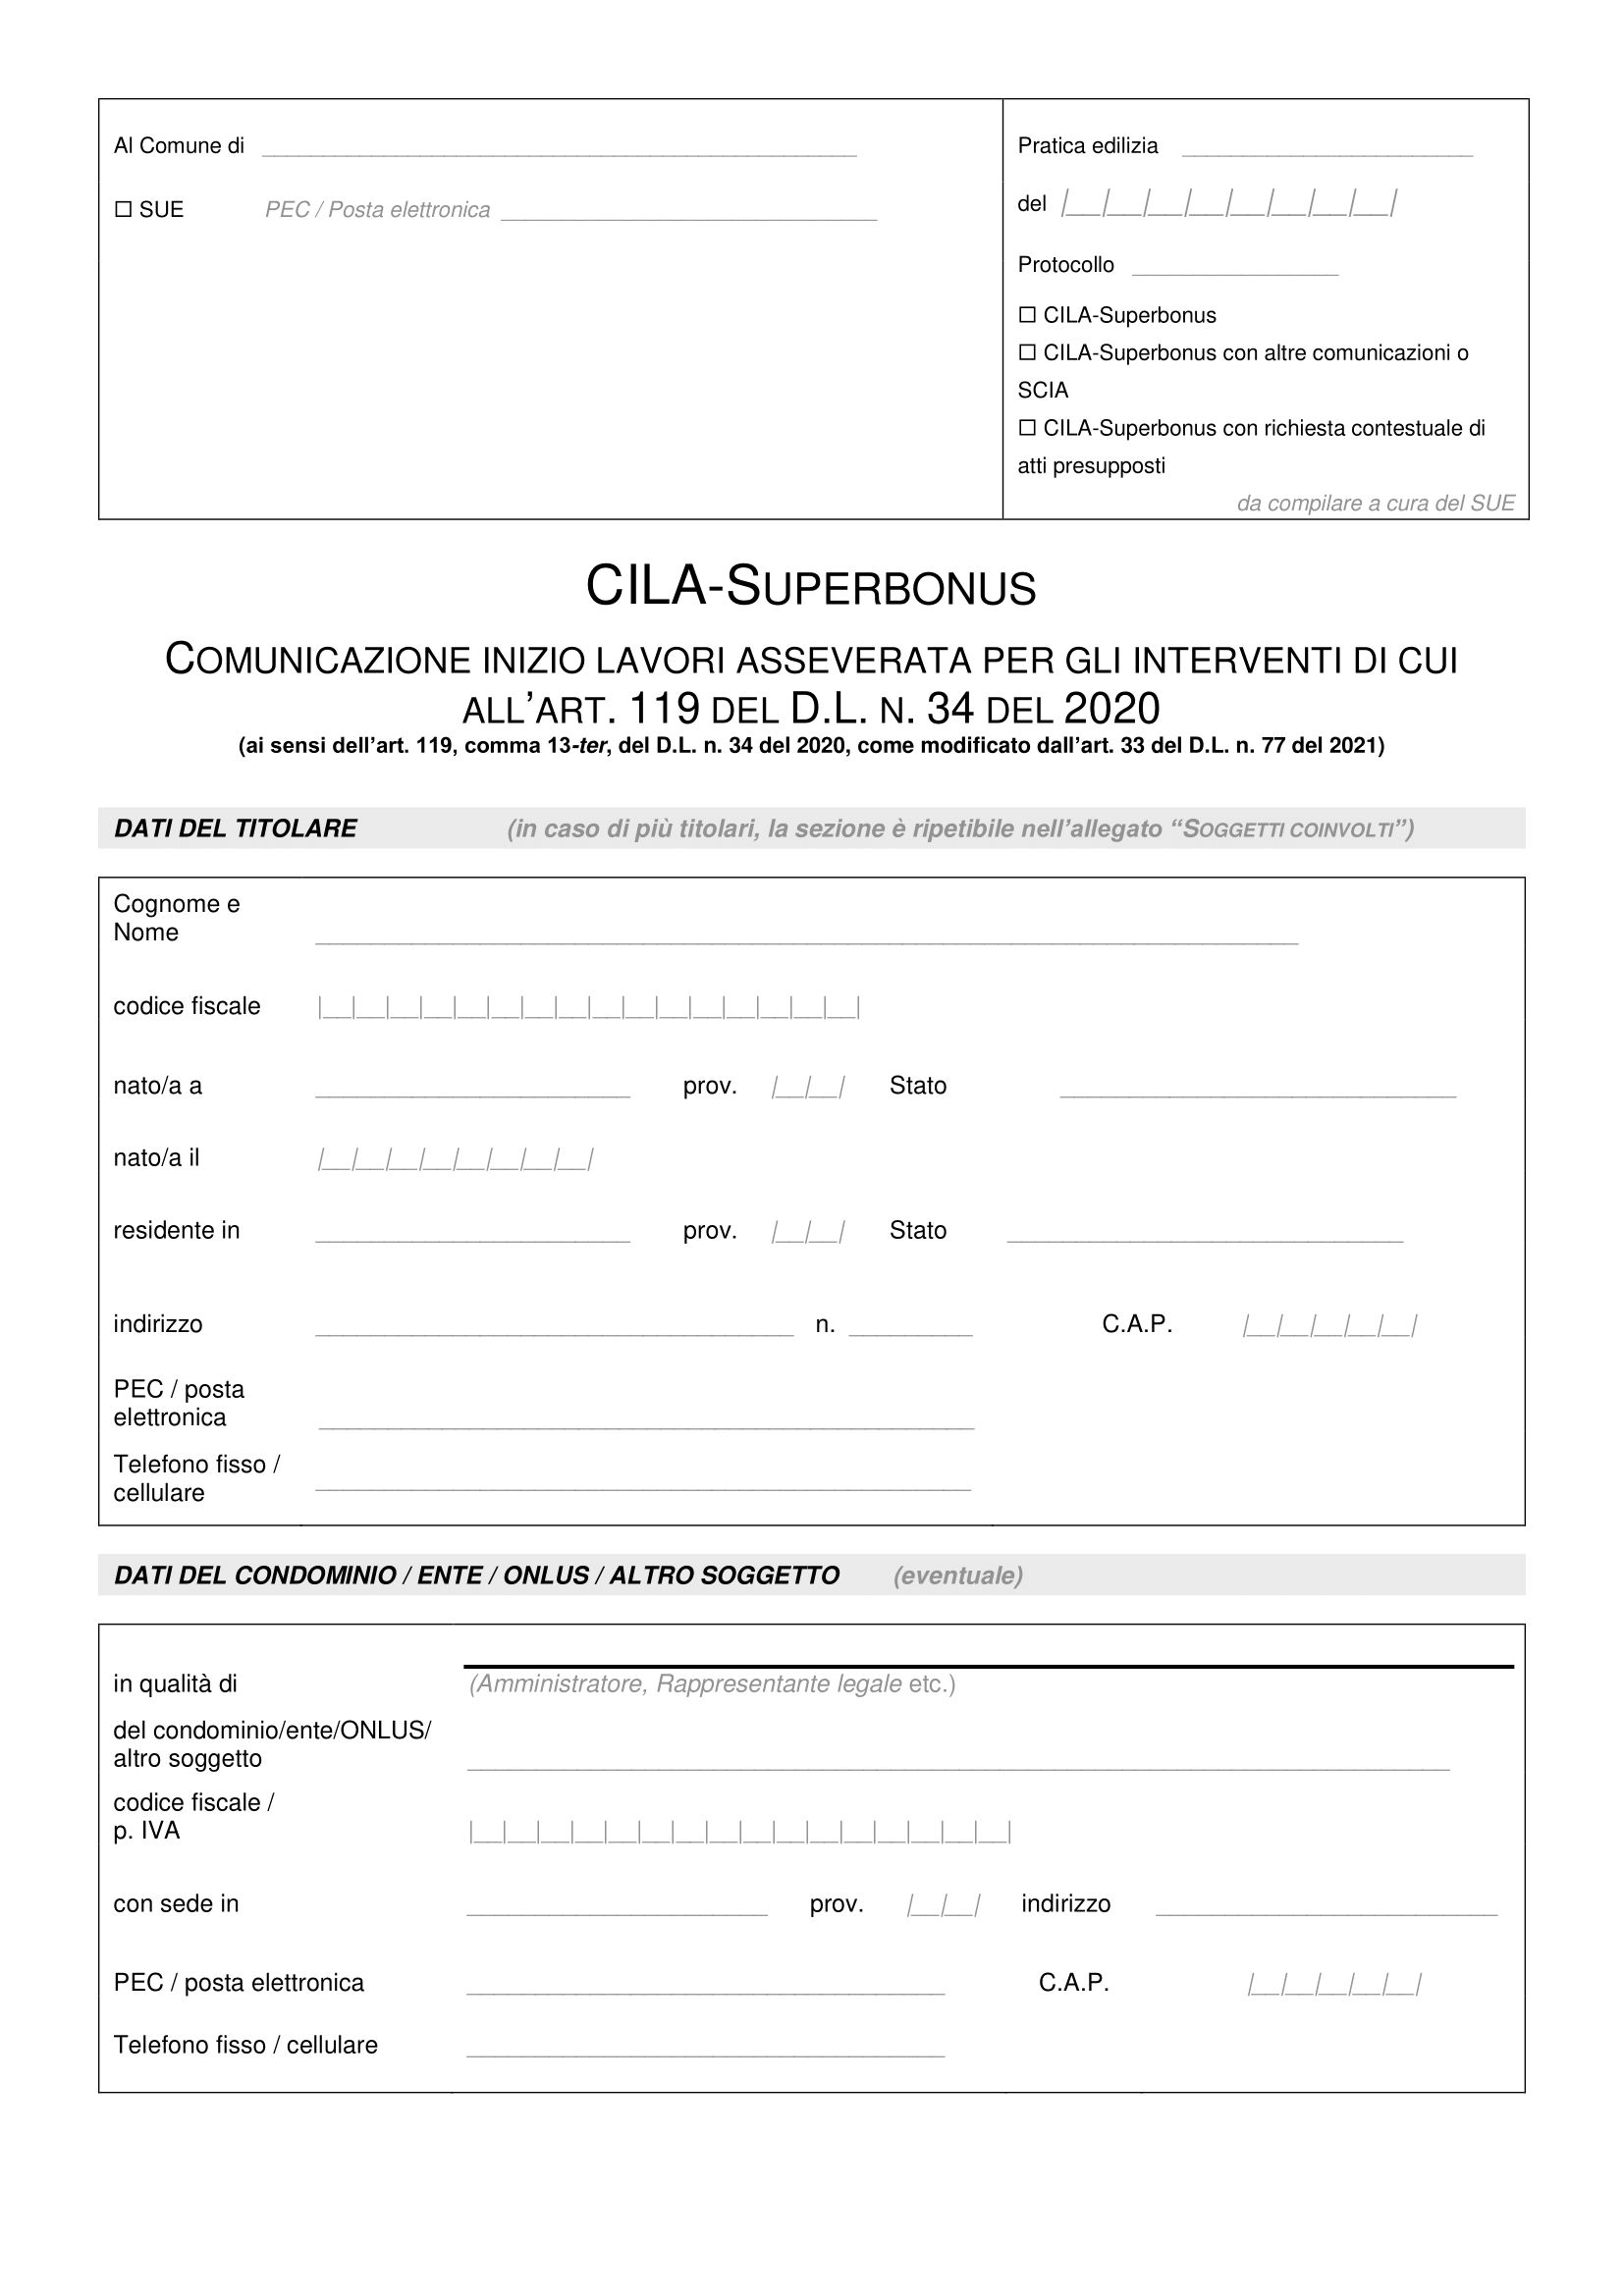
\includegraphics[scale=0.8]{../Img/Documents/CILAS/CILAS-1.png}
		\end{figure}
		\begin{figure}[H]
			\centering
			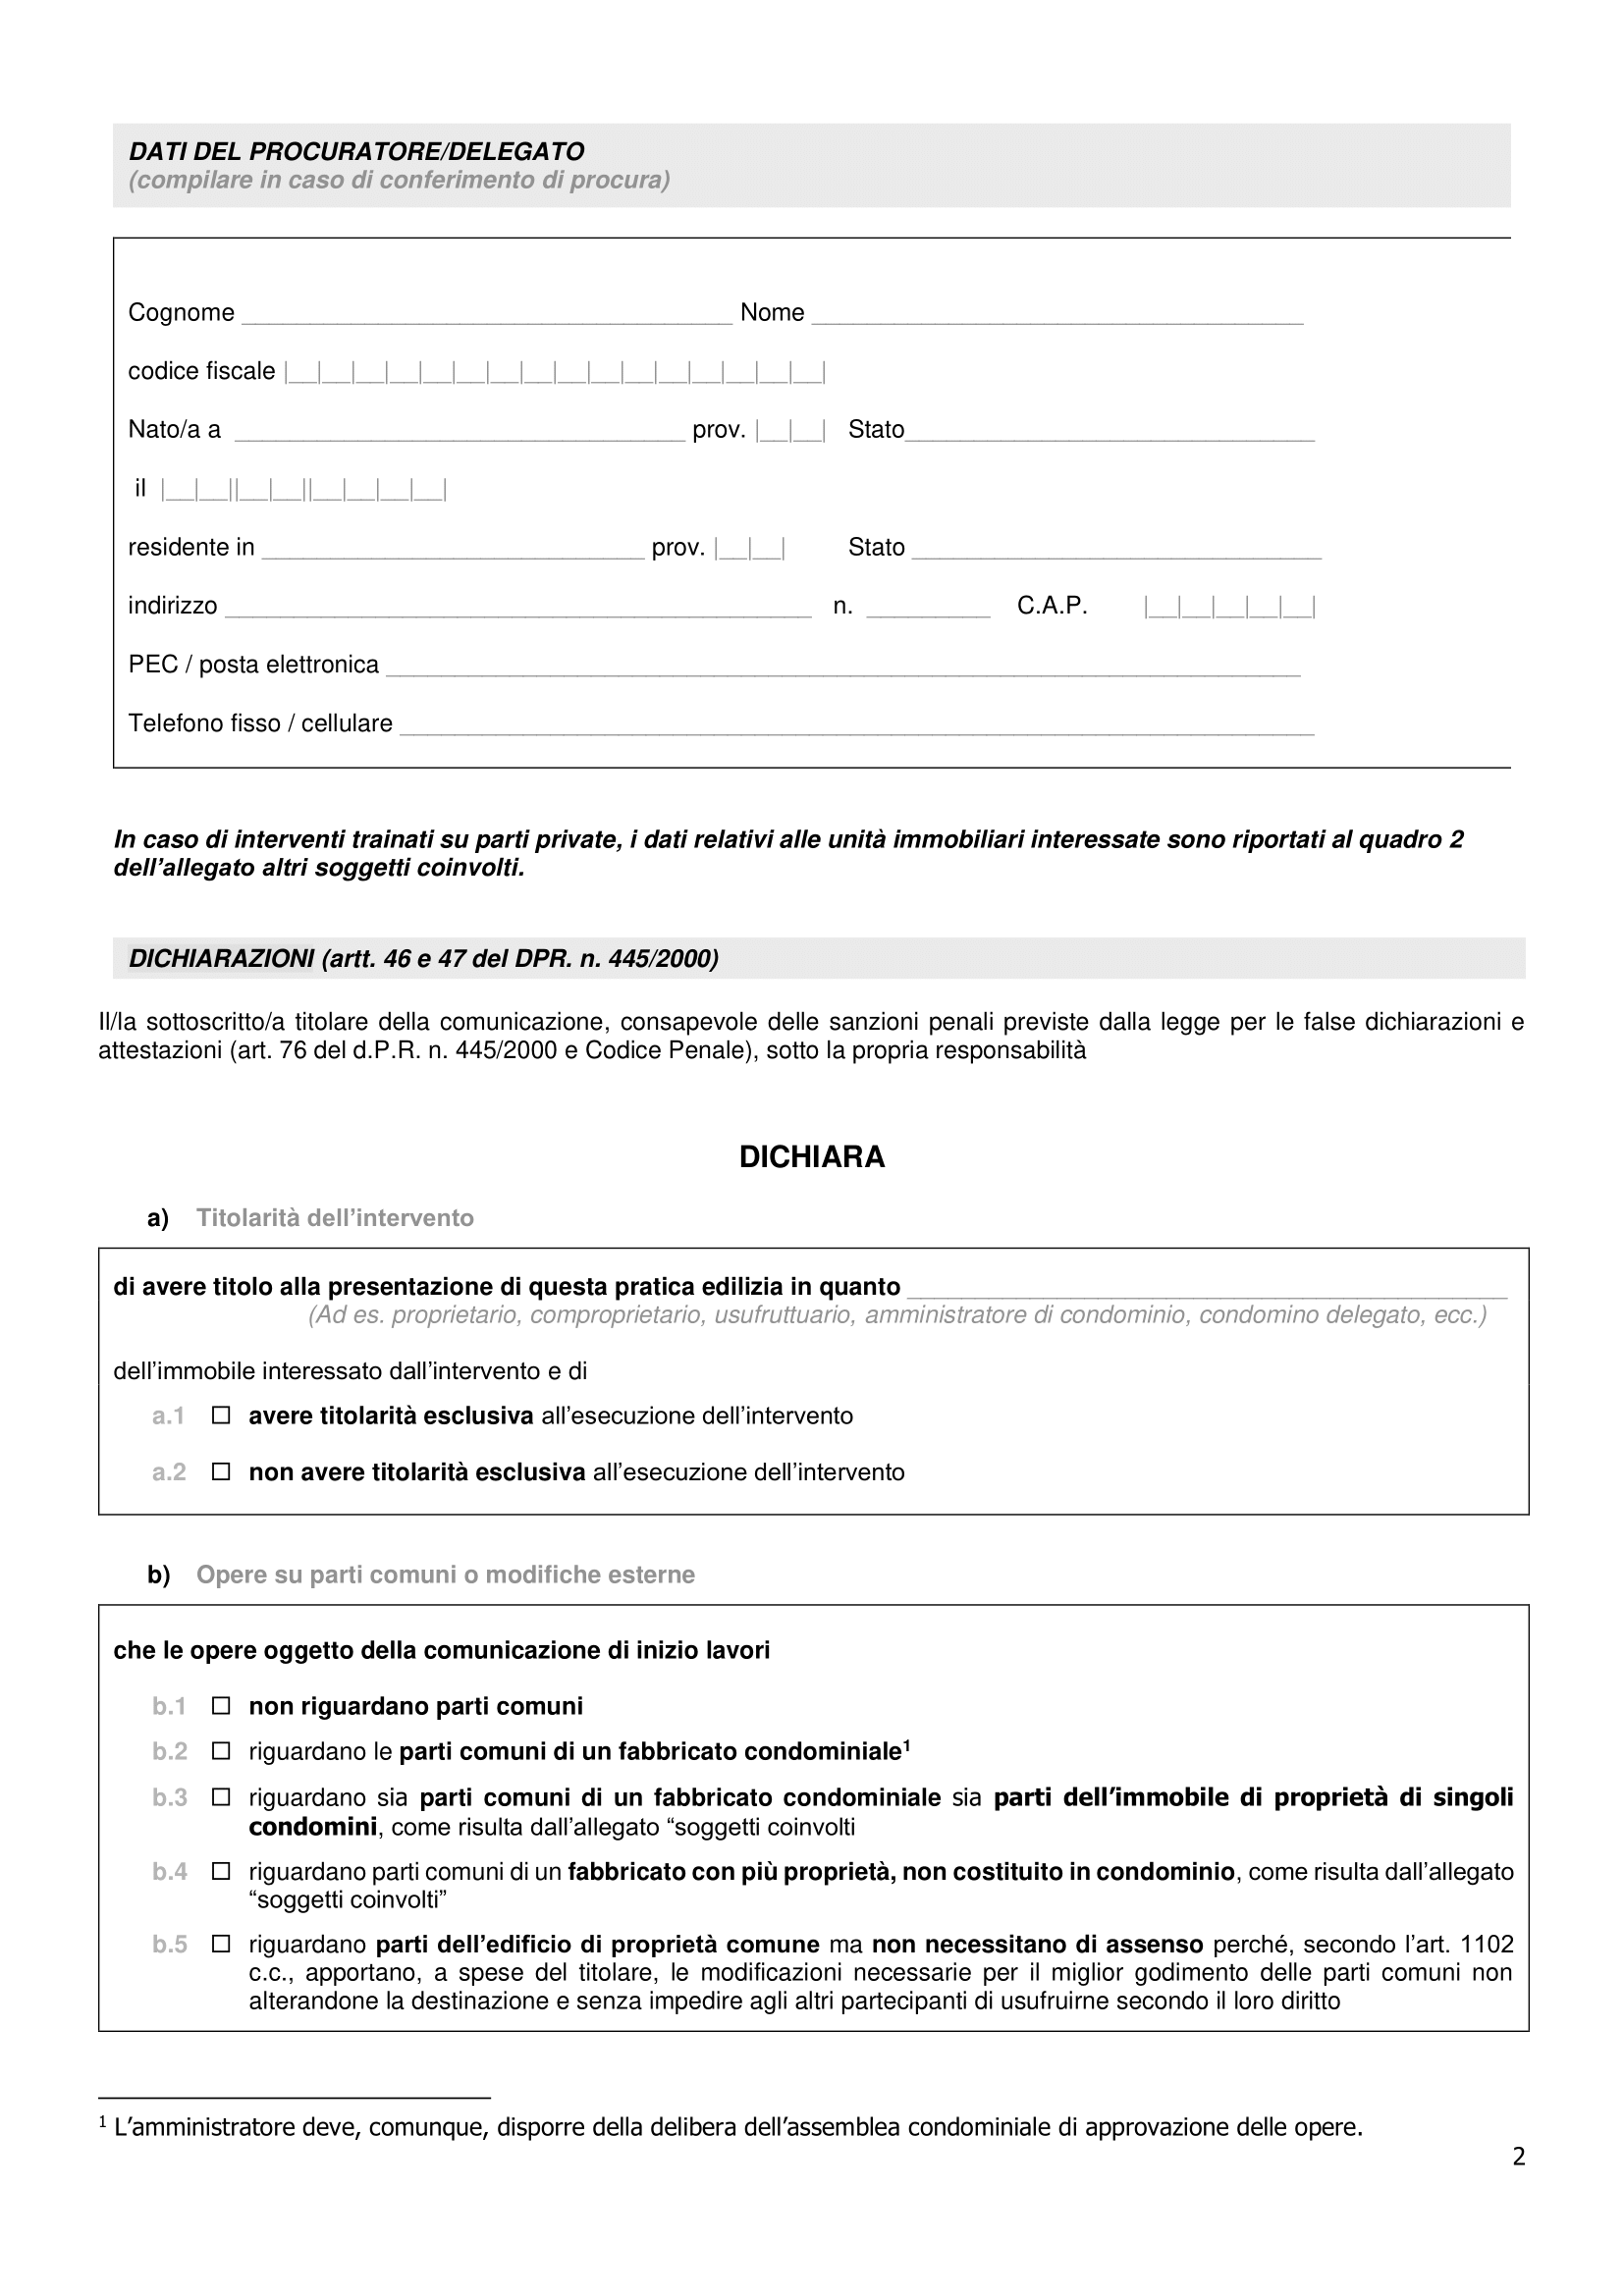
\includegraphics[scale=0.8]{../Img/Documents/CILAS/CILAS-2.png}
		\end{figure}
		\begin{figure}[H]
			\centering
			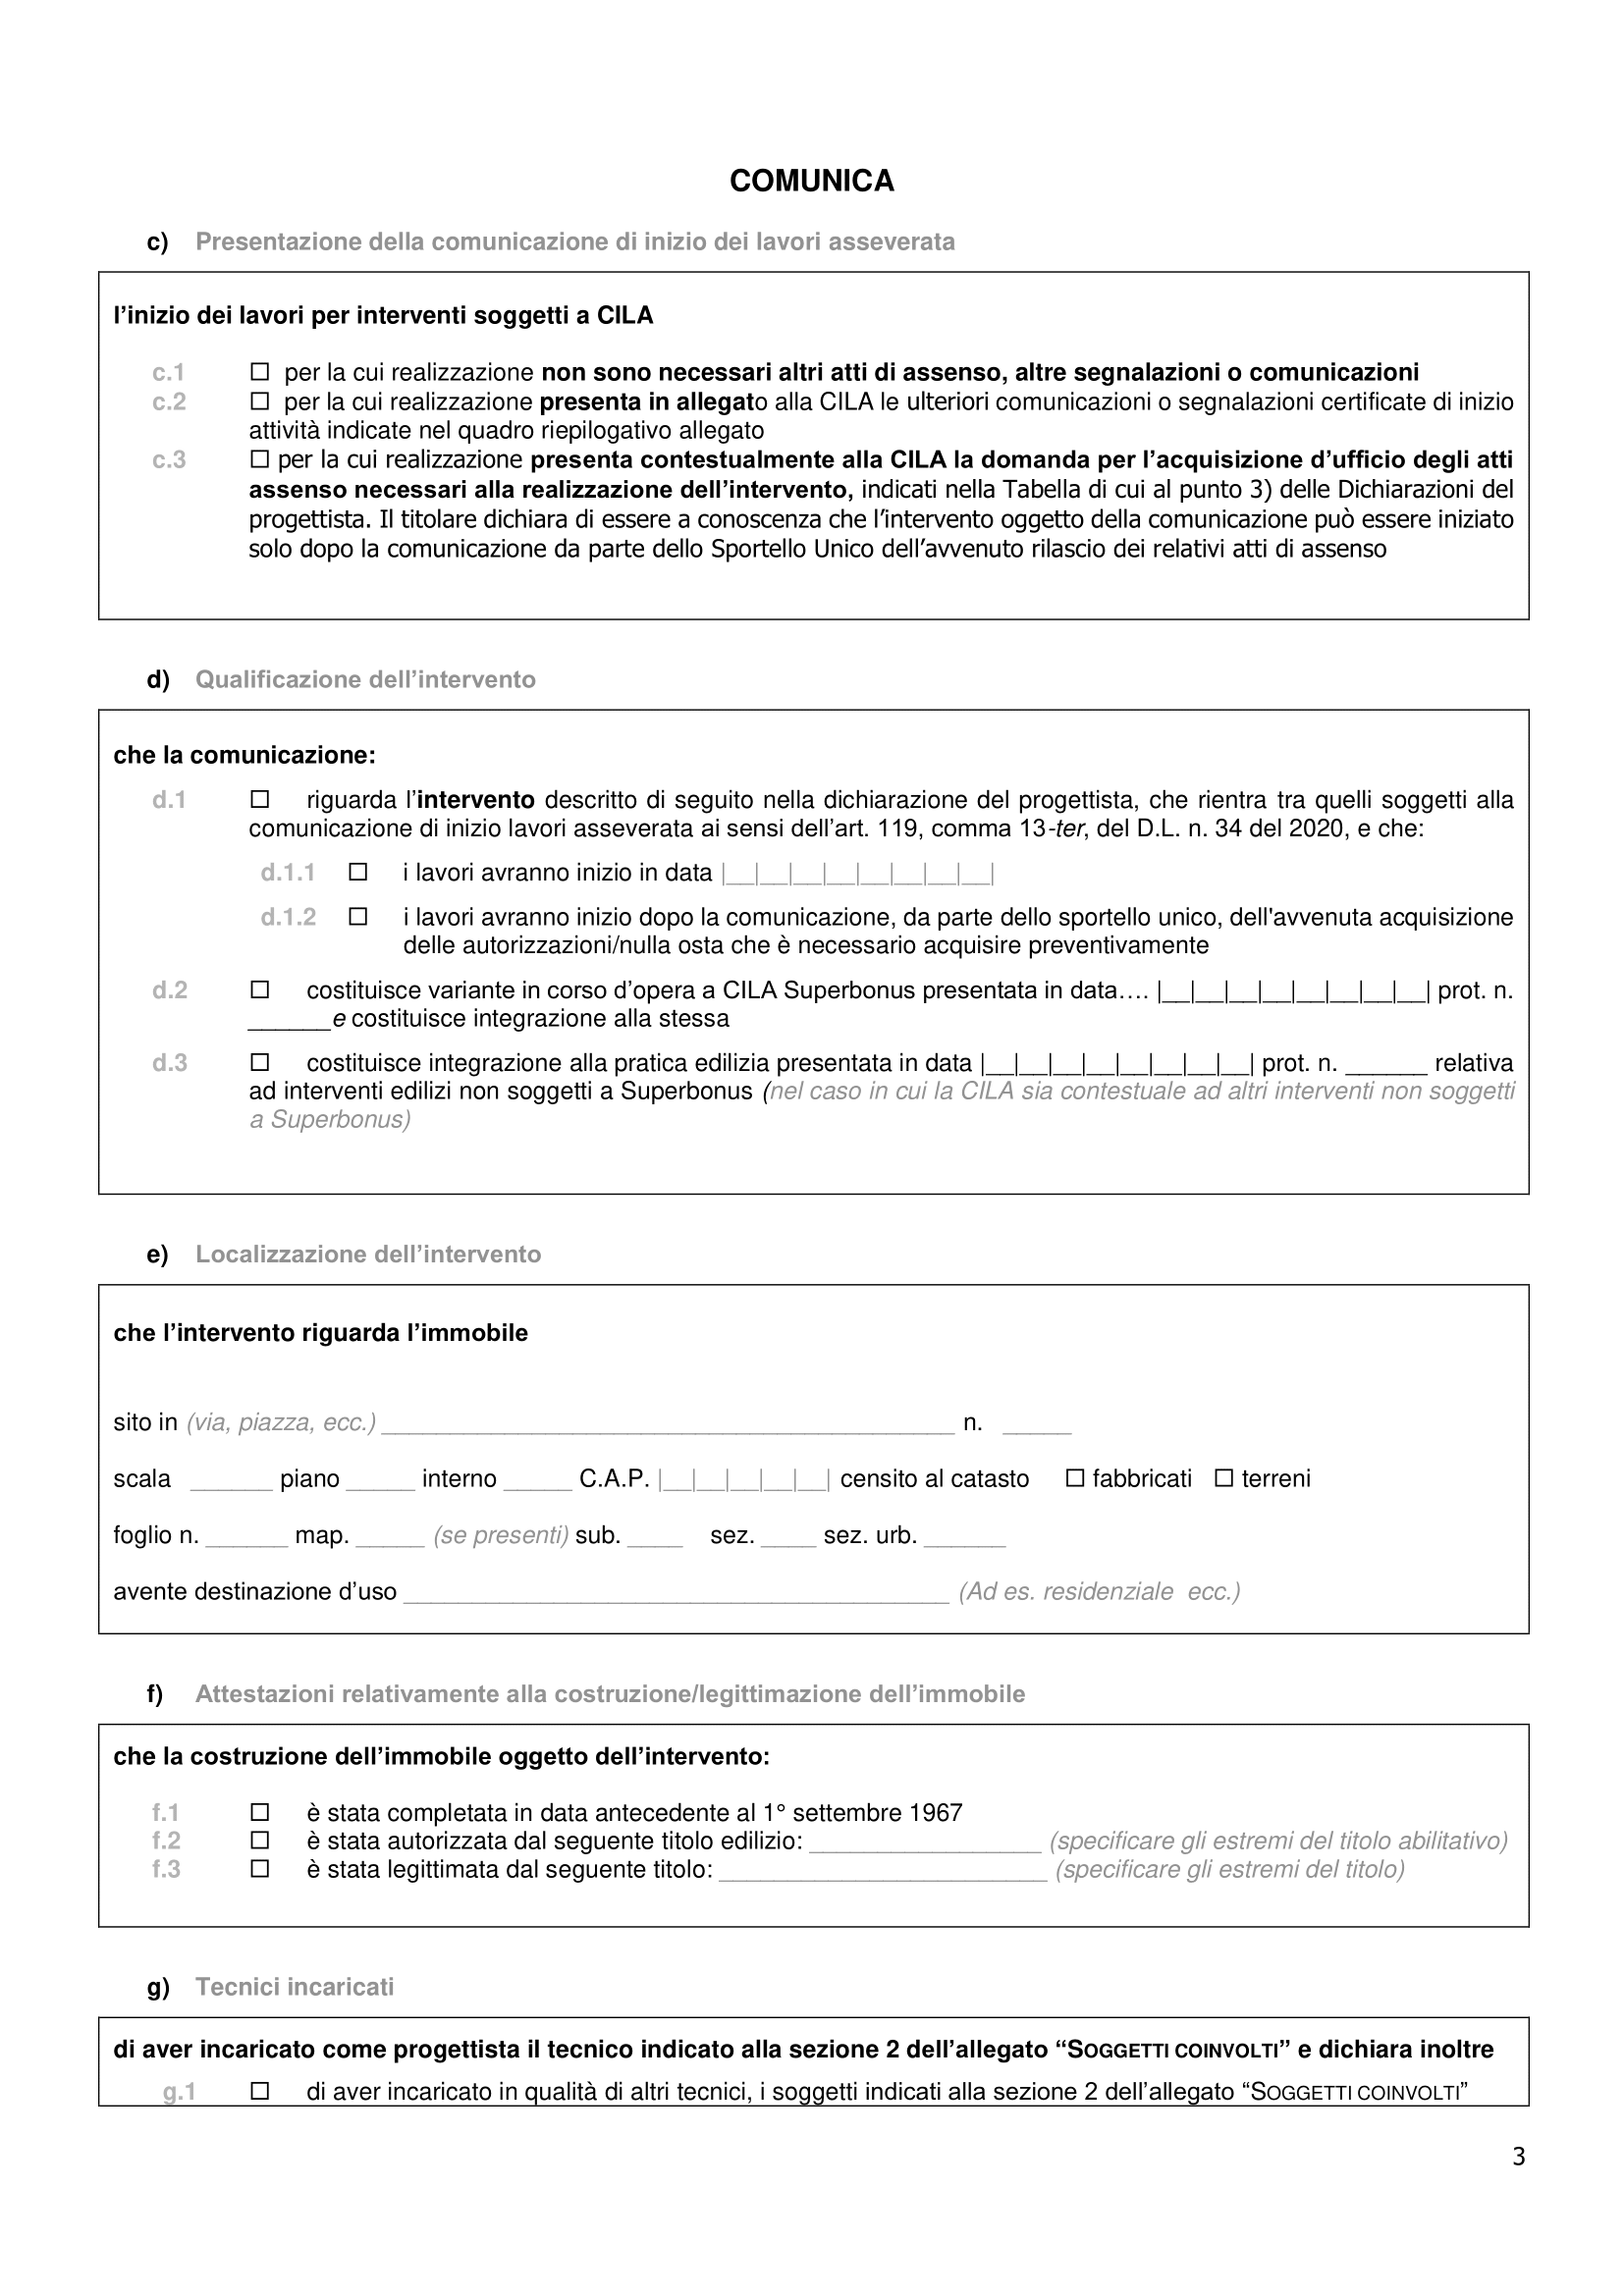
\includegraphics[scale=0.8]{../Img/Documents/CILAS/CILAS-3.png}
		\end{figure}
		\begin{figure}[H]
			\centering
			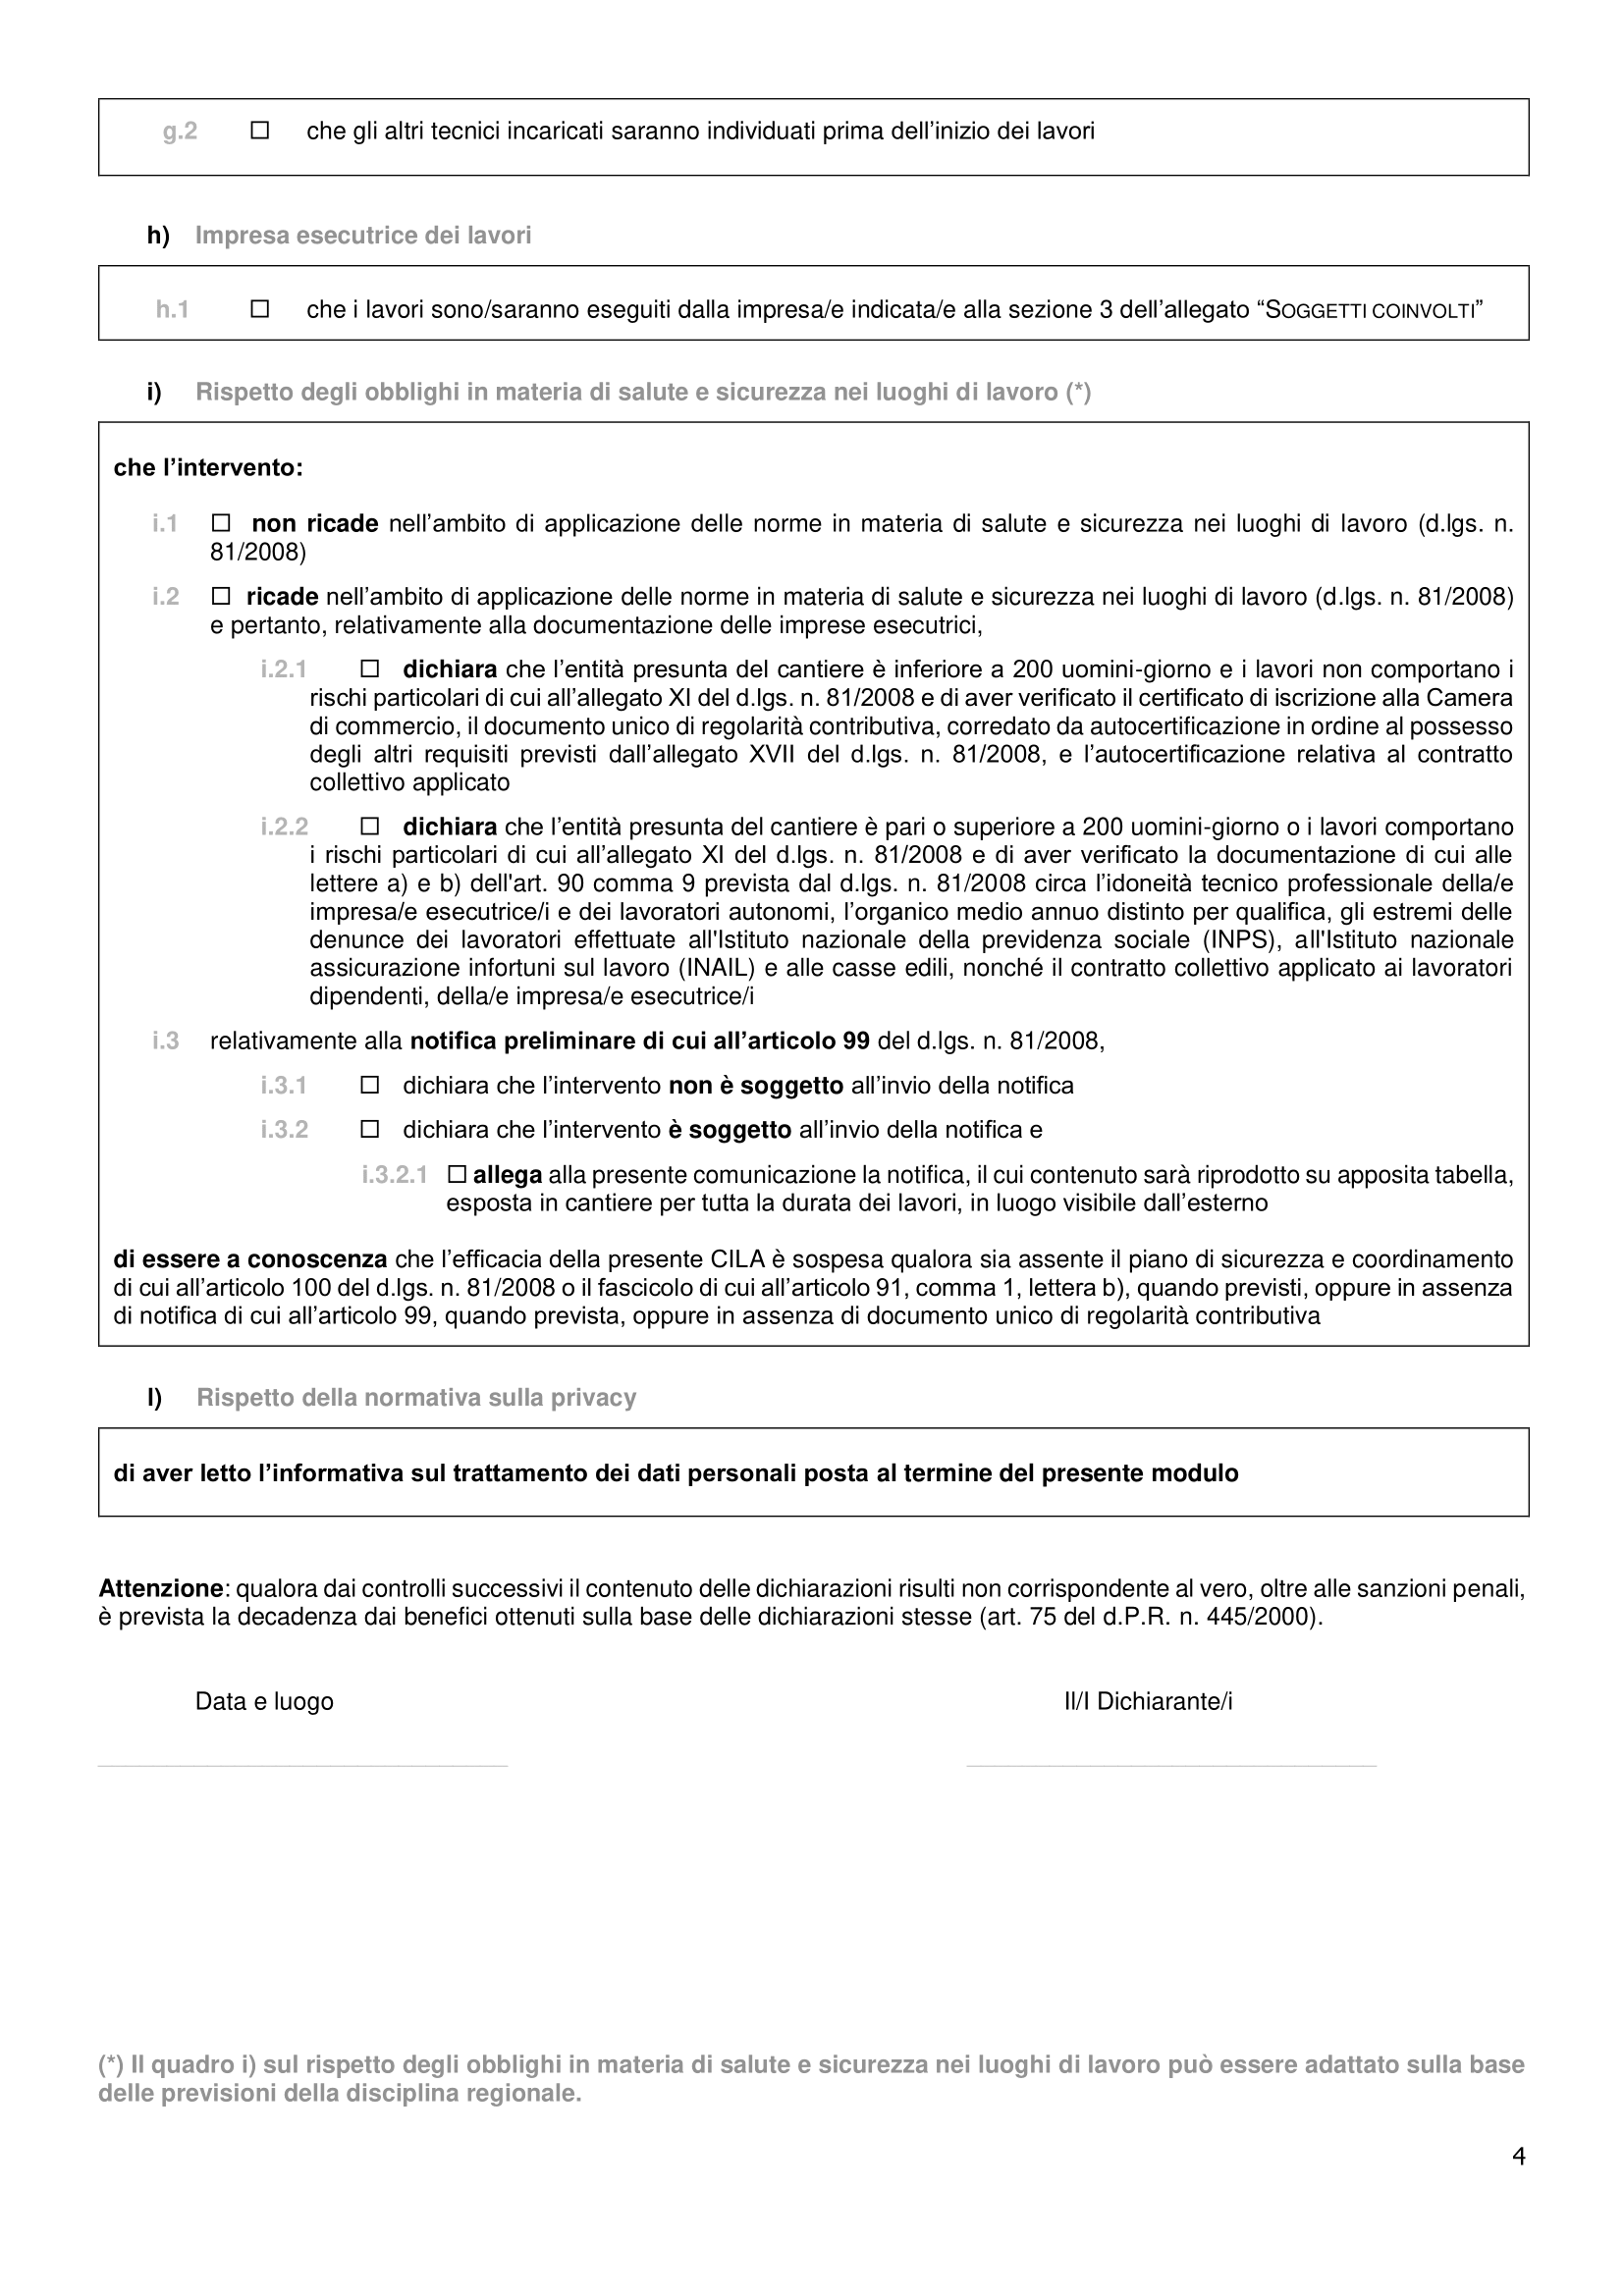
\includegraphics[scale=0.8]{../Img/Documents/CILAS/CILAS-4.png}
		\end{figure}
	\newpage
	\subsection{Comunicazione Fine Lavori}
	Documento di una CFL(Comunicazione Fine Lavori) utilizzato per raccogliere informazioni sui dati necessari.
		\begin{figure}[H]
			\centering
			
\includegraphics[scale=0.8]{../Img/Documents/CFL/CFL.png}
		\end{figure}
	\newpage	
	\section{Analisi dei Requisiti}
	\subsection{Analisi Processi Interni}
	Abbiamo rappresentato graficamente i cicli di vita dei processi interni all'azienda. I diagrammi sono stati realizzati in seguito ad una attenta analisi delle interviste.
	\subsubsection{Ciclo di vita di un progetto}
	\begin{figure}[H]
		\centering
		%[INSERISCI UN INVIO FATTURA SUL SI DEL CLIENTE HA PAGATO]
		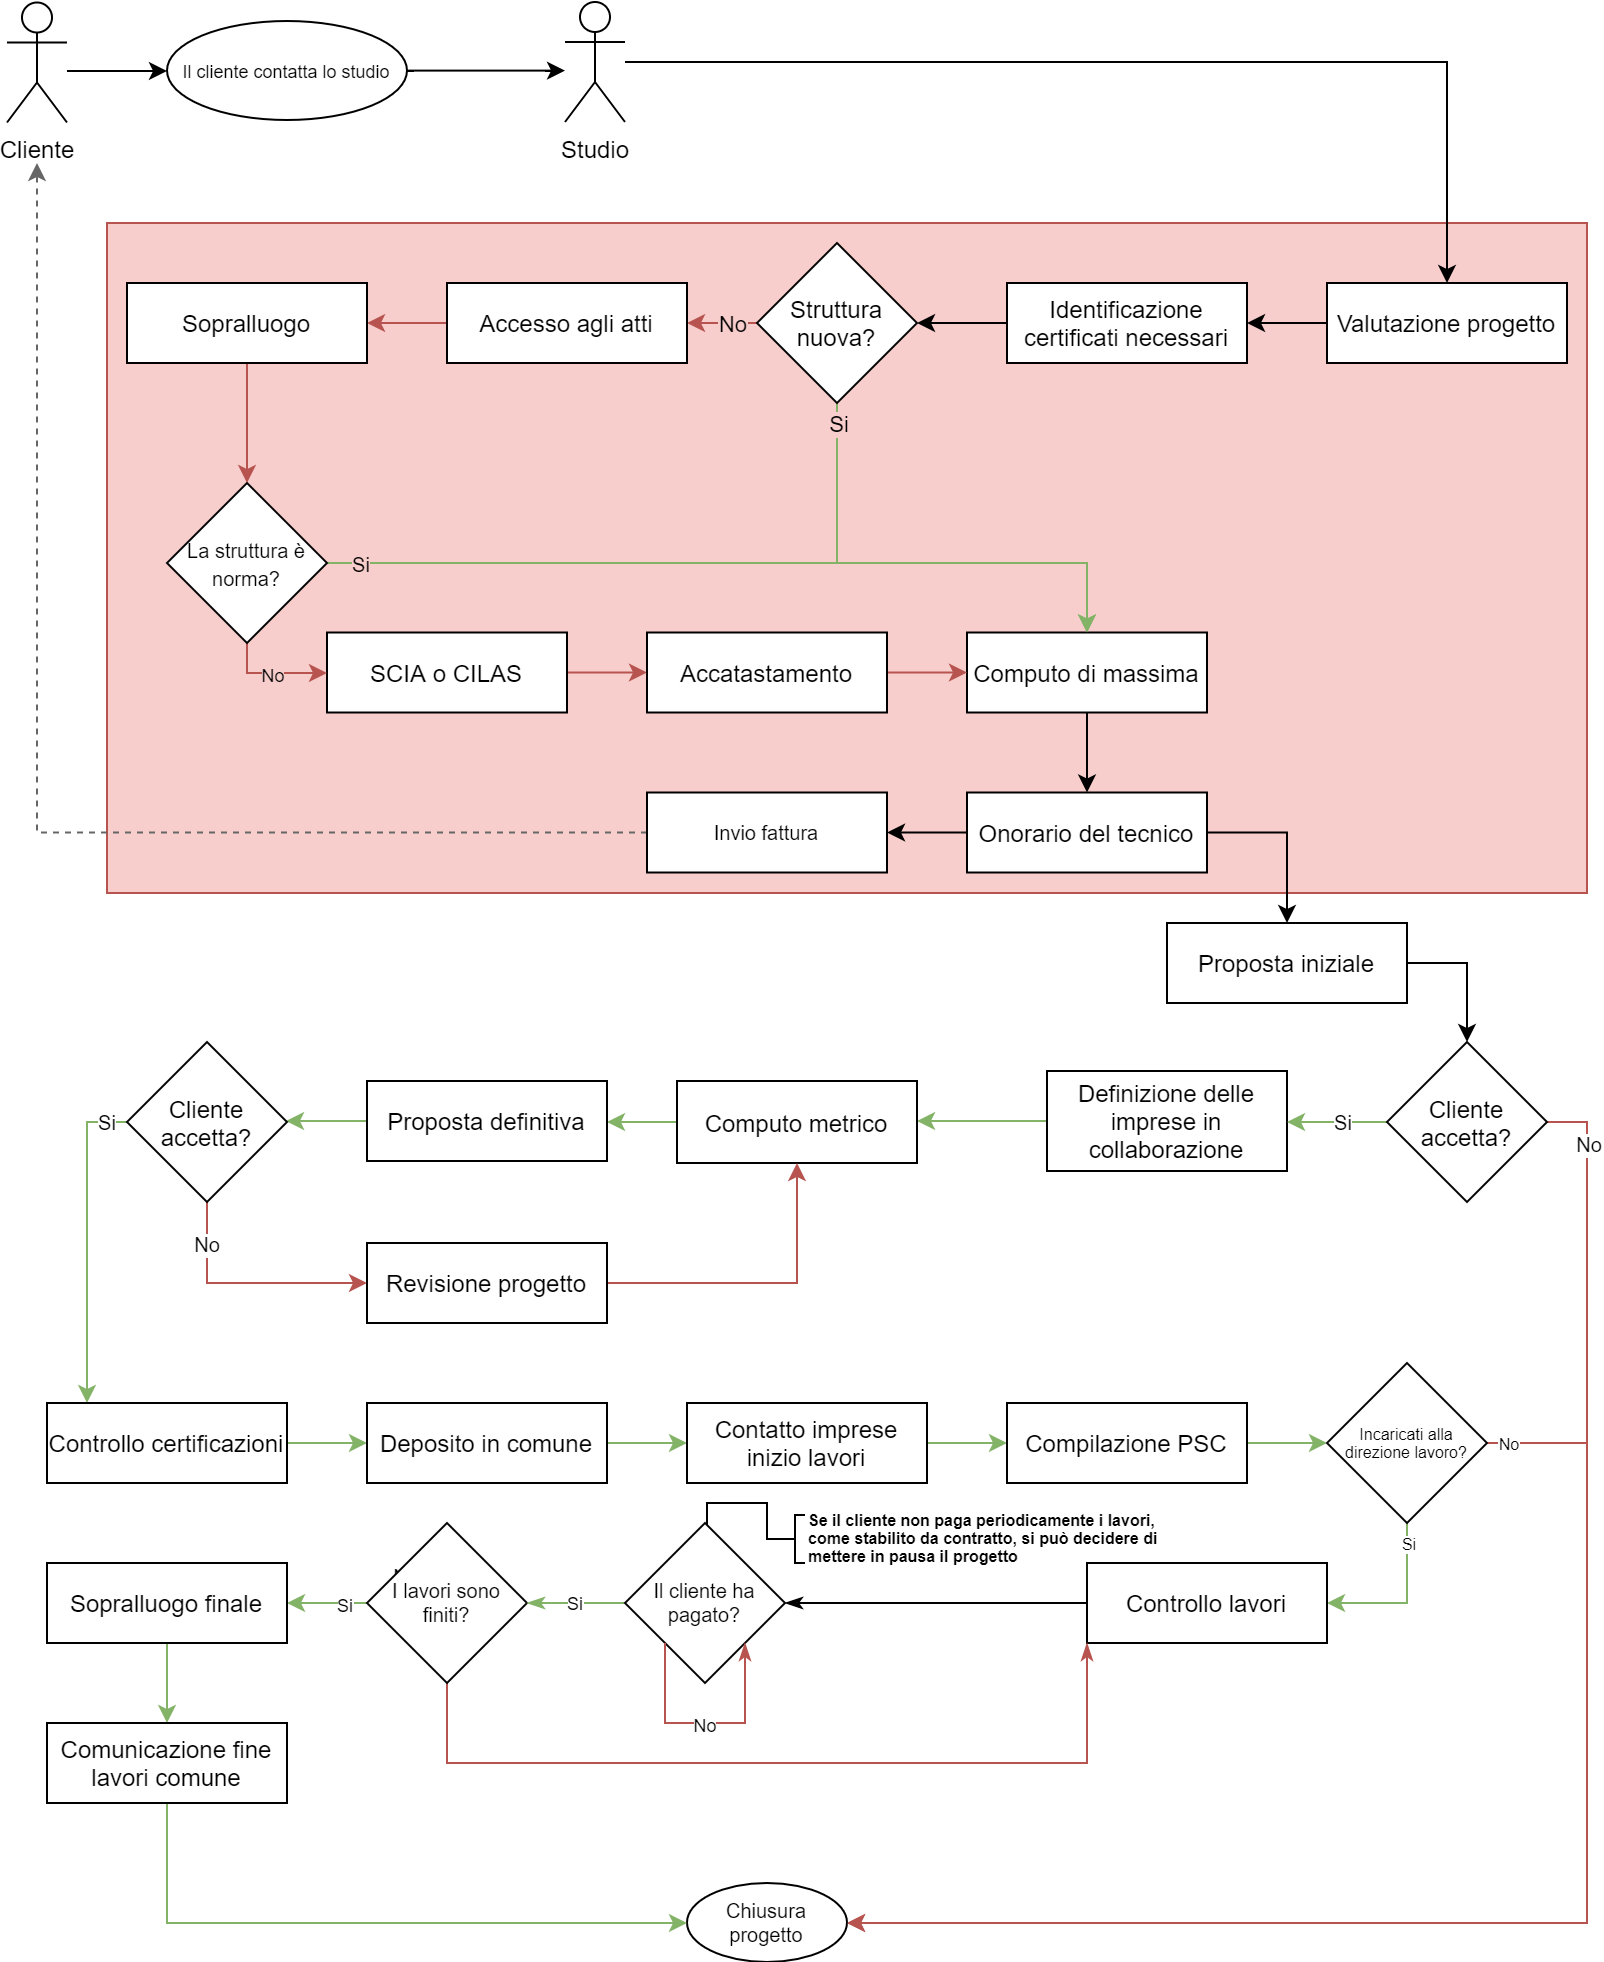
\includegraphics[scale=0.21]{../Img/Diagrams/diagram_flusso_progetto.png}
		\caption{Rappresentazione grafica del ciclo di vita di un progetto}
	\end{figure}
	\subsubsection{Ciclo di vita di una CTU/CTP}
	\begin{figure}[H]
		\centering
		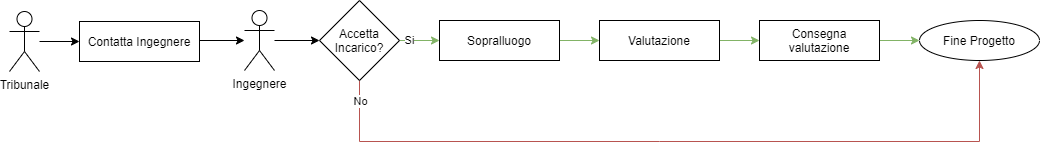
\includegraphics[scale=0.3]{../Img/Diagrams/diagram_flusso_progetto_2.png}
		\caption{Ciclo di vita di una consulenza legale}
	\end{figure}
	
	\subsection{Requisiti espressi in linguaggio naturale}
	
	In seguito ai dati raccolti dalle interviste e dalla documentazione, e dopo aver analizzato attentamente quest'ultimi,
        sintetizzando in concetti anche con schemi e tabelle, abbiamo definito quelli che sono i requisiti della base di dati.
	\\\\
	
	L'obiettivo è quello di realizzare una base di dati per uno Studio Ingegneristico per l'edilizia e l'architettura che 
        non solo realizza progetti, ma offre servizi come consulenze legali e certificazioni, che non sia troppo invasiva in 
        modo tale da poter mantenere intatto il loro flusso di lavoro, migliorando la gestione e semplificando dove necessario
        per dare una visione chiara dei processi svolti dagli ingegneri, permettendo quindi una migliore organizzazione e strutturazione dei dati.
	\\\\
	
	Si devono gestire tutti i dati relativi ai Progetti, ai Clienti (che possono essere Persona Fisica, Impresa o Condominio), alle
        Imprese con cui collaborano, e dunque le Collaborazioni, le Fatture, i Lavori ed i Tecnici dello Studio.
	\\\\
	
	Per quanto riguarda i \underline{\textbf{Clienti}} le informazioni che si devono conoscere dipendono dal tipo di cliente;
        se si tratta di un privato: il \textbf{nome}; il \textbf{cognome}; il \textbf{luogo e la data di nascita};
        il \textbf{codice fiscale}; la \textbf{residenza}; l'\textbf{email}; la \textbf{PEC}; il \textbf{numero di telefono}. Se, invece, si
        tratta di una società: la \textbf{denominazione}; la \textbf{sede legale}; il \textbf{codice fiscale} dell'impresa; la
        \textbf{partita IVA}; la \textbf{PEC}. Inoltre, bisogna tenere conto dei rappresentati delle aziende che sono clienti
        dello Studio: il \textbf{nome}; il \textbf{cognome}; il \textbf{luogo e la data di nascita}; il \textbf{codice fiscale};
        la \textbf{residenza}; l'\textbf{email}; il \textbf{numero di telefono}.
	\\\\
	
	Riguardo le \underline{\textbf{Strutture}} si deve conoscere: l'\textbf{identificativo catastale}; il \textbf{comune};
        l'\textbf{indirizzo}; i \textbf{proprietari} della struttura; il \textbf{tipo di struttura}, ovvero una descrizione della
        struttura, e la \textbf{destinazione d'uso}, che descrive il tipo di utilizzo che si fa della struttura.
	\\\\
	
	Riguardo ai \underline{\textbf{Progetti}} si deve conoscere: i dati relativi al \textbf{cliente}; i dati relativi alla
        \textbf{struttura}; i \textbf{proprietari della struttura}; il \textbf{tipo di lavoro} che lo studio deve svolgere.
        Poiché non esiste un numero finito di lavori possibili, i tecnici descrivono questo campo a parole loro. Inoltre, i
        tecnici si segnano se il tipo di lavoro è un lavoro \textbf{"nuovo"} o \textbf{"vecchio"}; la \textbf{data di inizio e
        la data di fine computo}, ovvero il periodo in cui si elabora il computo; i dati delle \textbf{società che collaborano},
        nel caso ce ne fossero, e di cosa si sono occupate. Per identificare i progetti, i tecnici nello studio danno un nome
        univoco ad ogni progetto. Inoltre, bisogna sapere: se la \textit{direzione lavori} è affidata allo studio o meno; in
        caso di progetto di "vecchio", la \textbf{data di inizio e la data di fine di accesso agli atti}; la
        \textbf{data di inizio e la data di fine dei sopralluoghi} effettuati, poiché questi vengono fatti durante un periodo
        preciso; i \textbf{file} legati al progetto.
	\\\\
	
	Riguardo le \underline{\textbf{Consulenze}} si deve conoscere: i dati del \textbf{cliente} che usufruisce del servizio;
        le informazioni relative alla \textbf{struttura}; i \textbf{tecnici} coinvolti;
        i \textbf{file} legati alla consulenza; 
	
	Nel caso delle CTU e CTP, che rientrano nelle Consulenze, si dovrà tenere conto degli avvocati coinvolti, quindi nome,
        cognome ed un contatto che può essere telefono, email o entrambi. Inoltre, esclusivamente per le CTU, il cliente è sempre un giudice.
	\\\\
	
	Riguardo le \underline{\textbf{Fatture}} si deve conoscere: il \textbf{numero di fattura}; il \textbf{Cliente}; la
        \textbf{Data di emissione della pre-fattura}; la \textbf{Data di emissione della fattura}; la \textbf{Data di Incasso};
        \textbf{Modalità} di pagamento; l'\textbf{Imponibile}; Il \textbf{Totale della fattura}, che si calcola imponendo
        all'imponibile prima la CNPAIA 4\% e poi l'IVA 22\% ; la \textbf{Ritenuta D'Acconto}; i \textbf{Costi Esenti IVA}; il
        \textbf{Totale Incassato}, che si calcola rimuovendo dal Totale della fattura prima il 4\% e poi il 22\%.
	
	Nel caso in cui la fattura è fatta per un progetto di ristrutturazione, si tiene conto anche della \textbf{Ritenuta della Banca}.
	\\\\
	
	Riguardo le imprese \underline{\textbf{Collaboratrici}} si deve conoscere: la \textbf{denominazione}; la \textbf{sede legale};	l'\textbf{email} di contatto; il numero di telefono.
	\\\\
	
	Riguardo ai \underline{\textbf{Tecnici dello Studio}} si deve conoscere: il \textbf{nome} e il \textbf{cognome}; la
        \textbf{email} e il \textbf{telefono}; le \textbf{certificazioni} possedute, ovvero il \textbf{il tipo di certificazione};
        il relativo \textbf{numero identificativo}.
	
	\subsection{Glossario dei Termini}
	\label{sec:Glossario}
	\begin{center}
		\small
		\begin{longtable}{|l|p{7cm}|l|p{3cm}|}
			\hline
			\textbf{Termine} & \textbf{Descrizione} & \textbf{Sinonimi} & \textbf{Collegamenti}\\
			\hline
			
			Accesso agli atti & Periodo nel quale lo studio accede ai documenti relativi ad una struttura & & Progetti\\
			\hline
			
			Progetto & Lavoro che prevede una fase di progettazione. &Lavoro & Imprese, Cliente, Fattura, Tecnico\\
			\hline
			
			Proprietario & Proprietario della Struttura & & Struttura\\
			\hline
			
			Cliente & Privato, azienda o ente pubblico che richiede un lavoro allo studio. & & Progetto, Fattura, Consulenza\\
			\hline
			
			Collaboratore & Società con cui lo studio collabora per portare a termine i progetti. & Società, ditta, azienda & Progetto\\
			\hline
			
			Fattura & Documento con le indicazioni della prestazione fornita, dell'ammontare dell'importo e delle
                        relative condizioni di pagamento. & & Progetto, Consulenza, Cliente\\
			\hline

			Consulenza & Lavoro che consiste in una valutazione. &Lavoro & Cliente, Tecnico, Fattura\\
			\hline
			
			Sopralluogo & Ispezione di una struttura a fini analitici. & & Progetto\\
			\hline
			
			Perizia di stima & Valutazione dedita allo stimare il valore economico-commerciale di una struttura.& Perizia & Cliente, Tecnico, Fattura\\
			\hline
			
			Tecnico & Ingegnere, geometra o architetto che lavora nello studio. & & Consulenza, Progetto\\
			\hline
			
			Certificato & Documento che certifica la competenza del tencio dello studio ad effettuare lavori di diverso tipo. & & Progetto, Tecnico \\
			\hline
			
			Catasto & Registro italiano dei beni immobili. & & Struttura\\
			\hline
			
			Identificativo catastale& Serie di valori che identificano una struttura all'interno del catasto. & & Struttura\\
			\hline
			
			Partita IVA & sequenza di 11 cifre che identifica univocamente un soggetto che esercita un'attività. & & Cliente, Fattura, Collaboratori\\
			\hline
			
			PEC & Posta Elettronica Certificata; email che permette di dare a un messaggio di posta elettronica lo stesso valore legale di una tradizionale raccomandata&&Cliente, Impresa\\
			\hline 
			
			Imponibile& L'importo su cui vengono applicate le tasse.&&Fattura\\
			\hline
			
			CME & Computo Metrico Estimativo: documento che permette di definire il costo di un operazione edilizia. & Computo &Progetto\\
			\hline
			
			CPI & Certificato Prevenzioni Incendi: documento che certifica che una struttura verifica di tutti i requisiti di sicurezza antincendio. & Antincendio & Progetto\\
			\hline
			
			PSC & Piano Sicurezza e Coordinamento: documento che coordina il lavoro delle ditte edili nel cantiere. & & Progetto\\
			\hline
			
			CTU & Consulente Tecnico d'Ufficio: lavoro di consulenza svolto per il giudice in un processo civile. & & Progetto\\
			\hline
			
			CTP & Consulente Tecnico di Parte: lavoro di consulenza svolto per una delle parti in un processo civile & & Progetto\\
			\hline
			
			SCIA & Segnalazione Comunicazione Inizio Lavori: dichiarazione che consente alle imprese di iniziare, modificare o cessare un’attività produttiva.  &  & Progetto\\
			\hline
			
			CILAS & Comunicazione Inizio Lavori Asseveramento Semplificata: dichiarazione che consente alle imprese di iniziare, modificare o cessare un’attività produttiva. Copre meno tipi di attività rispetto alla SCIA, ma risulta più semplice.& & Progetto \\
			\hline
		\end{longtable}
	\end{center}
	
	\subsection{Strutturazione dei requisiti}
	\subsubsection{Frasi di carattere generale}
	
	L'obiettivo è quello di realizzare una base di dati per uno Studio Ingegneristico per l'edilizia e l'architettura che non solo realizza progetti, ma offre servizi come consulenza legale e certificazioni, che non sia troppo invasiva in modo tale da poter mantenere intatto il loro flusso di lavoro, migliorando la gestione e semplificando dove necessario per dare una visione chiara dei processi svolti dagli ingegneri, permettendo quindi una migliore organizzazione e strutturazione dei dati.
	Si devono gestire tutti i dati relativi ai Progetti, ai Clienti, che possono essere Persona Fisica o Impresa, alle Imprese con cui collaborano, e dunque le Collaborazioni, le Fatture, i Lavori ed i Tecnici dello Studio.
	\subsubsection{Frasi relative ai Clienti}
	
	Per quanto riguarda i \underline{\textbf{Clienti}} le informazioni che si devono conoscere dipendono dal tipo di cliente; se si tratta di un privato:
	\begin{itemize}
		\item il \textbf{nome};
		\item il \textbf{cognome};
		\item il \textbf{luogo e la data di nascita}; 
		\item il \textbf{codice fiscale};
		\item la \textbf{residenza}; 
		\item l'\textbf{email};
		\item il \textbf{numero di telefono}.
		\item la \textbf{PEC}.
	\end{itemize}
	Se, invece, si tratta di una società:
	\begin{itemize}
		\item la \textbf{denominazione};
		\item la \textbf{sede legale};
		\item \textbf{codice fiscale} dell'impresa;
		\item la \textbf{partita IVA};
		\item la \textbf{PEC};
	\end{itemize}
        Inoltre, bisogna tenere conto dei rappresentati delle aziende che sono clienti dello Studio:
        \begin{itemize}
            \item il \textbf{nome};
            \item il \textbf{cognome};
            \item il \textbf{luogo e la data di nascita}; 
            \item il \textbf{codice fiscale};
            \item la \textbf{residenza}; 
            \item l'\textbf{email};
            \item il \textbf{numero di telefono}.
        \end{itemize}
	\subsubsection{Frasi relative alle Strutture}
	
	Riguardo le \underline{\textbf{Strutture}} si deve conoscere:
	\begin{itemize}
		\item l'\textbf{identificativo catastale};
		\item il \textbf{comune};
		\item l'\textbf{indirizzo};
		\item i \textbf{proprietari} della struttura;
		\item il \textbf{tipo di struttura}, ovvero una descrizione della struttura.
		\item la \textbf{destinazione d'uso}, che descrive il tipo di utilizzo che si fa della struttura.
	\end{itemize}
	
	\subsubsection{Frasi relative ai Progetti}
	
	Riguardo ai \underline{\textbf{Progetti}} si deve conoscere:
	\begin{itemize}
		\item i dati relativi al \textbf{cliente}.
		\item i dati relativi alla \textbf{struttura};
		\item i \textbf{proprietari della struttura}; 
		\item il \textbf{tipo di lavoro} che lo studio deve svolgere. Poiché non esiste un numero finito di lavori possibili, i tecnici descrivono questo campo a parole loro. Inoltre, i tecnici si segnano se il tipo di lavoro è un lavoro \textbf{"nuovo"} o \textbf{"vecchio"};
		\item la \textbf{data di inizio e la data di fine computo}, ovvero il periodo in cui si elabora il computo;
		\item i dati delle \textbf{società che collaborano}, nel caso ce ne fossero, e di cosa si sono occupate;
		\item i \textbf{file} legati al progetto.
	\end{itemize}
	
	Per identificare i progetti, i tecnici nello studio danno un nome univoco ad ogni progetto. Inoltre, bisogna sapere: se la \textit{direzione lavori} è affidata allo studio o meno; in caso di progetto di ristrutturazione, la \textbf{data di inizio e la data di fine di accesso agli atti}; la \textbf{data di inizio e la data di fine dei sopralluoghi} effettuati, poiché questi vengono fatti durante un periodo preciso.
	
	\subsubsection{Frasi relative alle Consulenze}
	
	Riguardo le \underline{\textbf{Consulenze}} si deve conoscere:
	\begin{itemize}
		\item i dati del \textbf{cliente} che usufruisce del servizio;
		\item le informazioni relative alla \textbf{struttura};
		\item i \textbf{tecnici} coinvolti;
		\item i \textbf{file} legati alla consulenza.
	\end{itemize}
	
	Nel caso delle CTU e CTP, che rientrano nelle Consulenze, si dovrà tenere conto degli avvocati coinvolti, quindi nome, cognome ed un contatto che può essere telefono, email o entrambi. Inoltre, esclusivamente per le CTU, il cliente è sempre un giudice;
	
	\subsubsection{Frasi relative alle Fatture}
	
	Riguardo le \underline{\textbf{Fatture}} si deve conoscere:
	\begin{itemize}
		\item il \textbf{numero di fattura};
		\item il \textbf{Cliente};
		\item la \textbf{Data di emissione della pre-fattura};
		\item la \textbf{Data di emissione della fattura};
		\item la \textbf{Data di Incasso};
		\item \textbf{Modalità} di pagamento;
		\item l'\textbf{Imponibile};
		\item Il \textbf{Totale della fattura}, che si calcola imponendo all'imponibile prima la CNPAIA 4\% e poi l'IVA 22\% ;
		\item la \textbf{Ritenuta D'Acconto};
		\item i \textbf{Costi Esenti IVA};
		\item il \textbf{Totale Incassato}, che si calcola rimuovendo dal Totale della fattura prima il 4\% e poi il 22\%.
	\end{itemize}
	
	Nel caso in cui la fattura è fatta per un progetto di ristrutturazione, si tiene conto anche della \textbf{Ritenuta della Banca}.
	
        \subsubsection{Frasi relative alle Imprese Collaboratrici}
	
	Riguardo le imprese \underline{\textbf{Collaboratrici}} con cui lo studio collabora si deve conoscere:
	\begin{itemize}
		\item la \textbf{denominazione};
		\item la \textbf{sede legale};
		\item l'\textbf{email} di contatto;
                \item il \textbf{numero} di telefono.
	\end{itemize}
	\subsubsection{Frasi relative ai Tecnici dello Studio}
	
	Riguardo ai \underline{\textbf{Tecnici dello Studio}} si deve conoscere:
	\begin{itemize}
		\item il \textbf{nome} e il \textbf{cognome};
		\item la \textbf{email} e il \textbf{telefono};
		\item le \textbf{certificazioni} possedute, ovvero il \textbf{il tipo di certificazione} e la relativa \textbf{data di scadenza};
	\end{itemize}
	
	\subsection{Eliminazione delle ambiguità presenti}
	Durante l'analisi abbiamo incontrato differenti termini ambigui, tra cui:
	\begin{itemize}
		\item Differenza tra Certificato per i Tecnici e Certificato sulle strutture. Con Certificato per i tecnici
                    intendiamo i certificati che abilitano il tecnico ad eseguire diverse tipologie di attività di consultazione,
                    in particolare, per lo Studio, si tratta di: antincendio, acustica ed energetica. Con Certificato sulle 
                    strutture si intendono i documenti che certificano determinati requisiti della struttura, ovvero antincendio,
                    acustica ed energetica. Il primo, dunque, abilita il tecnico a certificare che una struttura sia a norma,
                    mentre il secondo è un documento che assicura che una struttura sia a norma. Per questo motivo, abbiamo deciso
                    di rinominare il Certificato per i tecnici in \textbf{Attestato} e il Certificato sulle strutture in \textbf{Certificazione}.

		\item Lavori, progetti e consulenze: con il termine \textbf{Lavoro} viene inteso nel suo significato più ampio,
                    comprendendo sia i progetti che le consulenze. Il \textbf{progetto} è un lavoro fatto su una struttura,
                    "nuova" (e quindi da costruire) o "vecchia" (in genere una ristrutturazione), mentre con \textbf{Consulenza}
                    si intende un lavoro di consulenza legale.
	\end{itemize}

	\subsection{Specifica operazioni}
	\subsubsection{Premessa}
        Per una lista riordinata e riadattata allo schema concettuale finale, fare riferimento alla Tavola delle operazioni. La seguente lista è frutta di una prima analisi dei requisiti che sono mutati nel tempo, grazie ad un continuo dialogo con i dipendenti dello studio.
	Le seguenti operazioni sono state tratte dopo una attenta analisi dei requisiti, raccogliendo le 
        operazioni richieste direttamente dagli intervistati, discuttendone con lo studio ed aggiungendone altre che riteniamo essere di fondamentale importanza ai fini di un corretto uso del database. \\
	Le operazioni sono categorizzate in questo modo:
	\begin{itemize}
		\item Inserimento, operazioni che inseriscono un occorrenza di una entità; 
		\item Aggiunta: operazioni che inseriscono una occorrenza di relazione; 
                \item Aggiornamento: operazioni aggiornano una entità o relazione inserendo dati che in precedenza non erano presenti (Esempio: la data di conclusione di un Lavoro non è conosciuta a priori);
		\item Modifica: operazioni che modificano dati già presenti;
                \item Ricerca: operazioni che richiedono un input (anche) parziale per effettuare ricerche nel database;
		\item Consultazione: operazioni che richiedono un identificativo univoco;
		\item Cancellazione: operazioni che rimuovono occorrenze;
		\item Operazioni Specifiche: operazioni che eseguono un compito specifico e che non sono state raccolte nelle precedenti categorie.
	\end{itemize}
	
	Nota sulla differenza tra operazioni di Aggiornamento e operazioni di Modifica: nelle operazioni di aggiornamento non deve essere consentita la modifica di dati già presenti.
	\\
	Il volume delle operazioni viene contato in "media" annuale, mensile o giornaliera. In alcuni casi, dove non è possibile stimare una media, si utilizza il termine "al massimo", indicando il fatto che si tratta di una operazione che potrebbe anche non avvenire mai nell'arco di un anno, un mese o un giorno, ma al massimo potrebbe capitare un certo numero di volte o quando queste potrebbero essere eseguite solo in determinate condizioni.
	\\
	Inoltre, le seguenti operazioni sono pensate per essere eseguite da una applicazione (in particolare un 
        gestionale), e dunque, spesso, risultano essere generiche. Ad esempio: una operazione di aggiornamento di 
        una persona in un caso potrebbe aggiungere numero di telefono ed email, in un altro, invece, potrebbe 
        aggiungere i dati relativi alla residenza. Questo comportamento è espressamente richiesto dai tecnici 
        dello studio poiché le informazioni raccolte per ogni entità non avviene mai seguendo un ordine preciso e 
        non è mai detto che loro stessi ne siano a conoscenza fin da subito.
	\subsubsection{Lista Operazioni}
        \label{subsec:listOperazioni}
        \begin{enumerate}
		\item Aggiornamento Cliente, Condominio (al massimo 5 volte al mese)
		\item Aggiornamento Cliente, Persona (al massimo 5 volte al mese)
		\item Aggiornamento Collaboratore (al massimo 10 volte all'anno)
		\item Aggiornamento Fattura (20 volte al mese)
		\item Aggiornamento Struttura (70 volte all'anno)
		\item Aggiornamento di Consulenza, Certificato (35 volte all'anno)
		\item Aggiornamento di Consulenza, Consulenza Tecnica (48 volte all'anno)
		\item Aggiornamento di Consulenza, Perizia di Stima (20 volte all'anno)
		\item Aggiornamento di Progetto, data di fine accesso agli atti [NON ESPRIMIBILE solo se è già presente una data di inizio] (100 all'anno)
		\item Aggiornamento di Progetto, data di fine computo (95 all'anno)
		\item Aggiornamento di Progetto, data di fine sopralluoghi [NON ESPRIMIBILE solo se è già presente una data di inizio] (100 all'anno)
		\item Aggiornamento di Progetto, data di inizio accesso agli atti (100 all'anno)
		\item Aggiornamento di Progetto, data di inizio computo (95 all'anno)
		\item Aggiornamento di Progetto, data di inizio sopralluoghi (100 all'anno)
		\item Aggiunta Partecipazione di Tecnico a Lavoro (200 volte l'anno)
		\item Aggiunta di Amministratore di un condominio (al massimo 20 volte all'anno)
		\item Aggiunta di Coinvolgimento di una nuova struttura a progetto (al massimo 1 volta l'anno)
		\item Aggiunta di Collaborazione a progetto [richiede un lavoro ed un collaboratore] (80 volte l'anno)
		\item Aggiunta di Fattura [richiede un lavoro ed un cliente] (80 volte l'anno)
		\item Aggiunta di Impegno avvocato a consulenza tecnica (al massimo 8 volte al mese) [richiede un avvocato ed una consulenza]
		\item Aggiunta di Proprietario di struttura (5 volta l'anno)
		\item Aggiunta di Raprresentanza di un'impresa (10 volte l'anno)
		\item Aggornamento Cliente, Impresa (al massimo 5 volte al mese)
		\item Cancellazione Cliente, solo se non è mai stato coinvolto in un lavoro o se non posside una struttura (al massimo 1 volta all'anno)
		\item Cancellazione Collaborazione (al massimo 5 volte all'anno) 
		\item Cancellazione Fattura, solo se non ha una data di emissione (al massimo 1 volta al mese)
		\item Cancellazione Lavoro, solo se senza fattura (al massimo 10 volte all'anno)
		\item Concludi Lavoro, impedendo da questo momento in poi la modifica di qualunque dato relativo ad esso (80 volte l'anno)
		\item Consultazione Cliente (5 volte al giorno)
		\item Consultazione Lavori associati ad un Condominio (al massimo 10 volte al mese)
		\item Consultazione Lavori associati ad una Impresa (al massimo 10 volte al mese)
		\item Consultazione Lavori associati ad una Persona (al massimo 10 volte al mese)
		\item Consultazione Lavori che coinvolgono una Struttura (al massimo 10 volte al mese)
		\item Consultazione Progetto (100 volte al giorno)
		\item Consultazione Totale Fattura (20 al mese)
		\item Consultazione degli Attestati di un Tecnico (al massimo 10 volte all'anno)
		\item Consultazione dei Lavori relativi ad una Struttura (3 volte al mese)
		\item Consultazione dei Lavori svolti in un determinato periodo di tempo (al massimo 10 volte all'anno)
		\item Consultazione dei Progetti relativi ad una Struttura (3 volte al mese)
		\item Consultazione delle Abilitazioni di un Tecnico (al massimo 1 volta all'anno)
		\item Consultazione delle Consulenze relative ad una Struttura (3 volte al mese)
		\item Consultazione delle Fatture di un Lavoro (10 volte mese)
		\item Consultazione delle Fatture relative a un Cliente (al massimo 10 volte al mese)
		\item Consultazione di un Tecnico (al massimo 2 volta al mese)
		\item Consultazione di una Impresa (al massimo 20 volte al mese)
		\item Consultazione di una Struttura (5 volte al giorno)
		\item Inserimento di Nuova Consulenza, Consulenza Tecnica (al massimo 48 volte all'anno)
		\item Inserimento di Nuova Consulenza, Perizia di stima (20 volte l'anno)
		\item Inserimento di Nuova Struttura (80 volte l'anno)
		\item Inserimento di Nuovo Attestato (al massimo 1 volta l'anno) [richiede tecnico abilitato]
		\item Inserimento di Nuovo Avvocato (al massimo 8 volte al mese)
		\item Inserimento di Nuovo Collaboratore (al massimo 20 volte l'anno)
		\item Inserimento di Nuovo Consulenza, Certificato (30 volte l'anno) [richiede certificazione da parte di un tecnico abilitato a quel tipo di certificazione, il coinvolgimento di almeno una struttura ed un cliente]
		\item Inserimento di Nuovo Progetto(100 volte l'anno) [richiede coinvolgimento di almeno una struttura ed un cliente]
		\item Inserimento di Nuovo Tecnico (al massimo 3 volte l'anno)
		\item Modifica Persona, Dati di residenza, Numero di telefono e email (al massimo 10 volte all'anno)
		\item Modifica Tecnico, email di un tecnico (al massimo 2 volte all'anno)
		\item Modifica Tecnico, numero di telefono di un Tecnico (al massimo 2 volte all'anno)
		\item Modifica Valore stimato di una Perizia di Stima (al massimo 5 volte all'anno)
		\item Modifica di Progetto, Direzione Lavori (al massimo 15 volte all'anno)
		\item Modifica di un Avvocato, Email e Telefono (al massimo 5 volte all'anno)
		\item Modifica la Denominazione di un Lavoro (al massimo 10 volte all'anno)
		\item Ricerca Condominio per amministratore (al massimo 10 volte al mese)
		\item Ricerca Condominio per composizione di Comune, Provincia, Città, Indirizzo, CAP e numero Civico (al massimo 10 volte al mese)
		\item Ricerca Impresa per Denominazione (30 volte al mese)
		\item Ricerca Impresa per Rappresentante (10 volte al mese)
		\item Ricerca Lavori per Denominazione (30 volte al giorno)
		\item Ricerca Persona per Nome e Cognome (al massimo 30 volte al mese)
		\item Visualizza Lavori conclusi (al massimo 5 volte al mese)
		\item Visualizza Lavori in Corso (50 volte al giorno)
		\item Visualizza Progetti relativi a Progettazione di "vecchio" (10 volte al giorno)
                \item Calcolo del totale incassato per i lavori di un determinato tipo effettuati per un determinato cliente in un certo periodo (20 volte all'anno)
                \item Consultazione dei Lavori di certificazione che hanno necessitato di un Lavoro di messa a norma (20 all'anno)
                \item Consultazione dei Lavori svolti in un determinato comune (20 volte all'anno) 
                \item Consultazione dei collaboratori che hanno lavorato in una struttura (20 volte all'anno)
                \item Consultazione dei file relativi ad una Struttura (20 volte al mese)
                \item Consultazione delle fatture non incassate (20 volte all'anno)
                \item Consultazione delle strutture di un determinato cliente che hanno delle certificazioni in scadenza in questo anno (20 volte all'anno)
                \item Inserimento di Nuovo Cliente, Condominio (al massimo 10 volte l'anno) [richiede un amministratore di condominio]
                \item Inserimento di Nuovo Cliente, Persona (60 volte l'anno) 
                \item Inserimento di Nuovo File (20 volte al giorno) [Richiede un Lavoro]
                \item Modifica di Progetto (al massimo 30 volte all'anno)
                \item Numero di lavori a cui ha partecipato un tecnico in un anno categorizzandoli per tipo (5 volte all'anno)
                \item Statistica dei clienti per cui sono stati effettuati più lavori in un determinato periodo di tempo (20 volte all'anno)
                \item Statistica dei collaboratori che hanno partecipato più spesso ai lavori dello Studio categorizzandoli per il tipo di lavoro svolto (20 volte all'anno)
                \item Statistica dei comuni per cui sono stati svolti più lavori raggruppandoli per tipo di lavoro (20 volte alla'anno)
	\end{enumerate} 

	\chapter{Progettazione Concettuale}
	\section{Modalità con le quali procederemo}
        Analizzando tutti i dati raccolti dalle interviste e dalla documentazione che ci é stata fornita, abbiamo notato che le
        entità che entrano in gioco, da un punto di vista di alto livello, hanno tra di loro molti aspetti in comune che possono
        essere raggruppati in "macro entità": ad esempio, se pur differenti sotto alcuni punti di vista, \textit{Progetti} e
        \textit{Consulenze} sono comunemente legati ad un cliente e ad un o più fatture poiché entrambe le entità sono definiti 
        come \textit{Lavori}. Questa premessa ha come conseguenza diretta la definizone stessa delle relazioni tra le entità, che 
        verranno poi mano a mano a formarsi scendendo sempre più in profondità nei dettagli.
        Da queste macro entità che siamo riusciti a definire, abbiamo deciso di proseguire con la strategia top-down andando a raffinarle.
        Data la grande quantità di attributi che ci sono stati forniti, procederemo con raffinamenti di tipo bottom-up per accertarci della
        correttezza delle entità.
        Riteniamo dunque che la strategia mista sia il miglior approccio per questo progetto.
        
        Come primo passo, indentificheremo le principali entità su cui si fonderà e si svilupperà l'intero schema. Dopo di che, individueremo anche
        le principali relazioni tra di loro, formando cosi uno schema scheletro minimale.

        A questo punto, applicheremo la strategia top-down allo scheletro ottenuto, partendo da una visione di insieme che va mano a mano
        ad ampliarsi, per poi applicare la strategia bottom-up, per assicurarci che lo schema sia consistente, data la quantità di dati da conoscere,
        e per integrare i requisiti esprimibili solo ad un livello di dettaglio più approfondito.

	\section{Identificazione entità e relazioni}
        La prima fase consiste nella individuazione delle entità e delle loro relazioni fondamentali del preogetto: 

        \begin{figure}[H]
            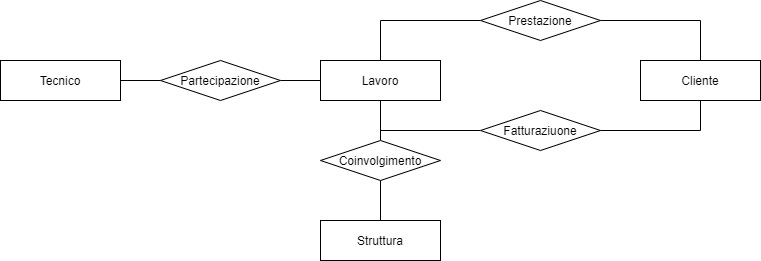
\includegraphics[width=15cm]{../Img/DBSchemes/scheletro.png}
            \caption{Entità fondamentali e scheletro}
        \end{figure}
        
        \textbf{Lavoro}: è l'entità che contiente tutto ciò che viene considerato, appunto, un lavoro, come ad esempio un progetto di ristrutturazione
        oppure una perizia.

        \textbf{Cliente}: é l'entità che rappresenta gli individui o le organizzazioni che richiedono una prestazione di servizio allo Studio.

        \textbf{Tecnico}: é l'entità che descrive i tecnici e il loro coinvolgimento nei vari lavori, oltre che a contenere le informazioni riguardanti
        le varie abilitazioni che può avere.

        \textbf{Struttura}: é l'entità che rappresenta le singole strutture interessate da uno o più lavori.

	\section{Sviluppo delle componenti dello scheletro}
        In questa sezione mostriamo come abbiamo sviluppato le entità fondamentali documentando come abbiamo proceduto nella loro realizzazione. 
            \subsection{Lavoro}
            Il primo passo dello sviluppo di \textbf{Lavoro} é il raffinamento di lavoro in \textbf{Progetti} e \textbf{Consulenze}:
            
            \begin{figure}[H]
                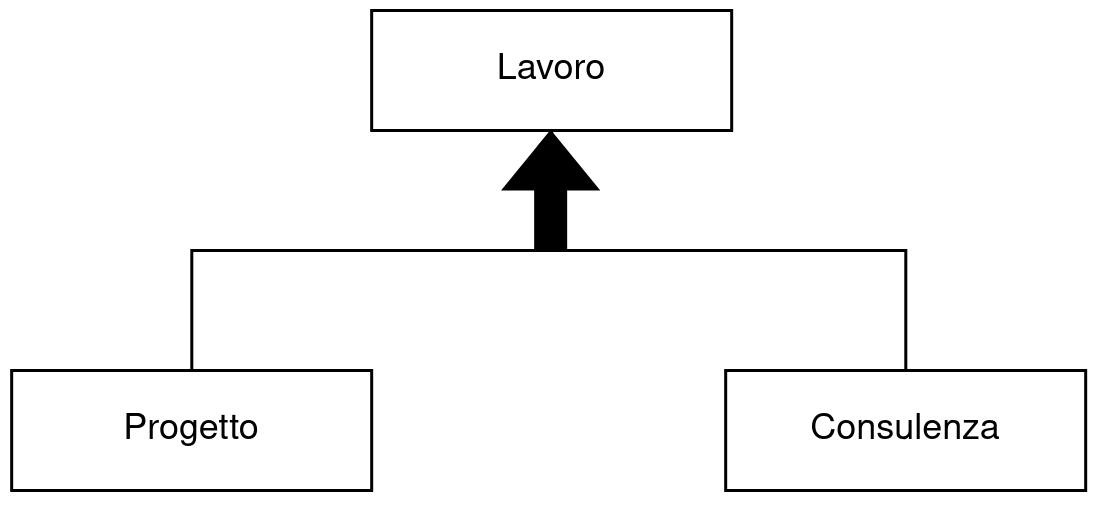
\includegraphics[scale=0.4]{../Img/DBSchemes/lavoro-1.png}
            \end{figure}
        
            Questa generalizzazione nasce in modo naturale poiché i due tipi di lavoro sono fondamentalmente differenti sia concettualmente che a livello di attributi. Nel primo
            si comprendono i lavori che hanno a che fare con progettazione di nuove strutture o di ristrutturazioni in generale, mentre nel secondo caso abbiamo lavori che comprendono
            consulenze tecniche o perizie che non prevodono una fase di progettazione.

            A loro volta le consulenze possono essere raffinate in \textbf{Consulenze Tecniche}, \textbf{Certificazione} e \textbf{Perizie}.\\
            Con \textbf{Consulenze Tecniche} intendiamo le consulenze svolte in un processo civile dove vengono coinvolti anche degli avvocati.\\
            Con \textbf{Certificazioni} si intendono i lavori dove si attesta che una struttura rispetti determinati requisiti.\\
            Con \textbf{Perizie} si intendnono le consulenze volte a stimare il valore di una struttura o di un danno. 

            \begin{figure}[H]
                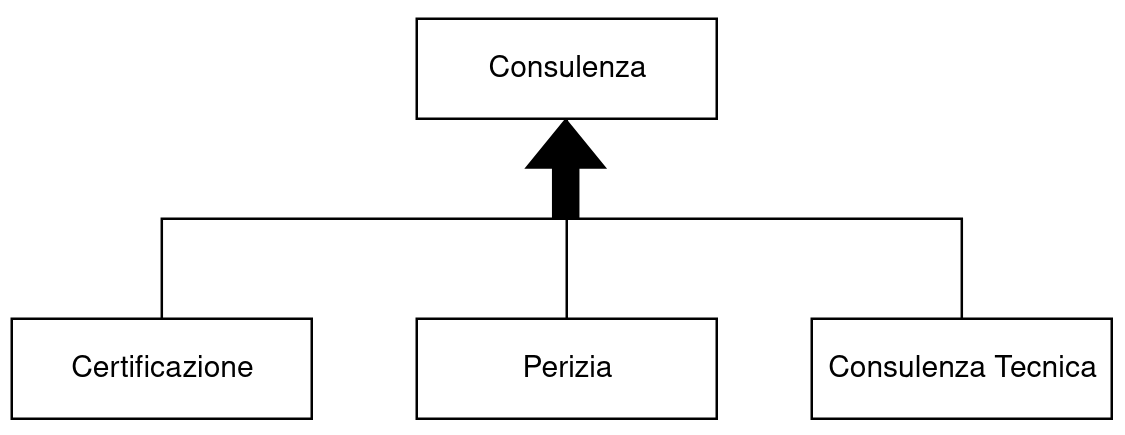
\includegraphics[scale=0.4]{../Img/DBSchemes/lavoro-3.png} 
            \end{figure}

            Allo stesso modo possiamo raffinare i \textbf{Progetti} in:\\
            \textbf{Nuovo}: progettazione di nuove strutture.\\
            \textbf{Vecchio}: progettazione su strutture già esistenti (come, ad esempio, ristrutturazioni).\\
            
            \begin{figure}[H]
                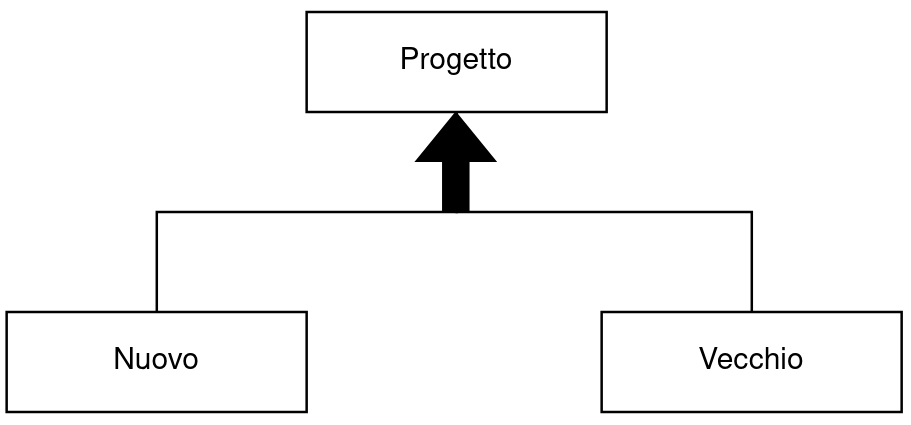
\includegraphics[scale=0.4]{../Img/DBSchemes/lavoro-2.png} 
            \end{figure}

           	Poiché tra le consulenze di diverso tipo non risultano attributi in comune, abbiamo deciso di eliminare la generalizzazione Consulenza. Abbiamo aggiunta una relazione tra \textbf{Progetto} e \textbf{Certificazione} per tener traccia di eventuali progetti di normalizzazione che sono stati eseguiti per il conseguimento di una certificazione.
           	Abbiamo quindi ottenuto il seguente schema:

            \begin{figure}[H]
                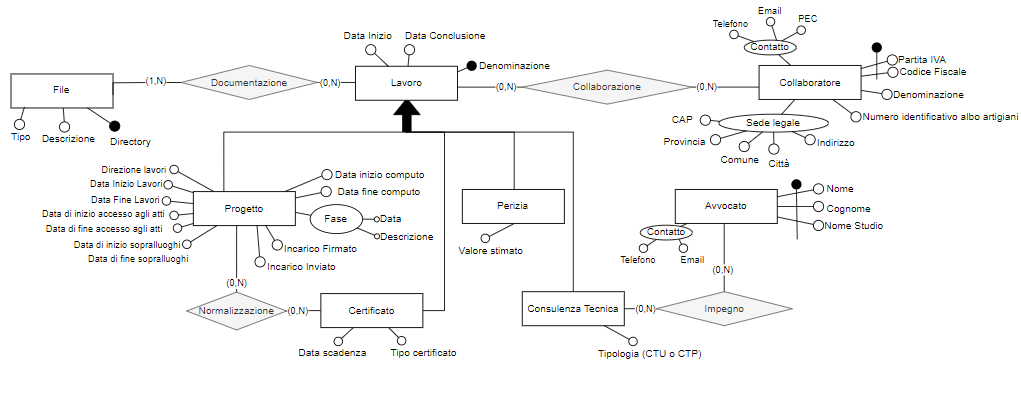
\includegraphics[scale=0.7]{../Img/DBSchemes/lavoro-completo.png} 
                \caption{Schema parziale sviluppato partendo da Lavoro}
            \end{figure}

            Abbiamo aggiunto \textbf{Avvocato} poiché, nei lavori di consulenza tecnica é sempre coinvolto almeno un avvocato ti cui si vuole tenere traccia, e l'entità \textbf{Collaboratore}
            che, invece, rappresenta quelle imprese che possono prendere parte ad una collaborazione per un progetto.
            Abbiamo inoltre aggiunto l'entità \textbf{File} per poter organizzare documenti e file di progettazione inerenti al progetto.
            
			\newpage
            \subsection{Cliente}
            In primo luogo, abbiamo deciso di specializzare l'entità cliente in \textbf{Privato} e \textbf{Giudice}.
            
            \begin{figure}[H]
                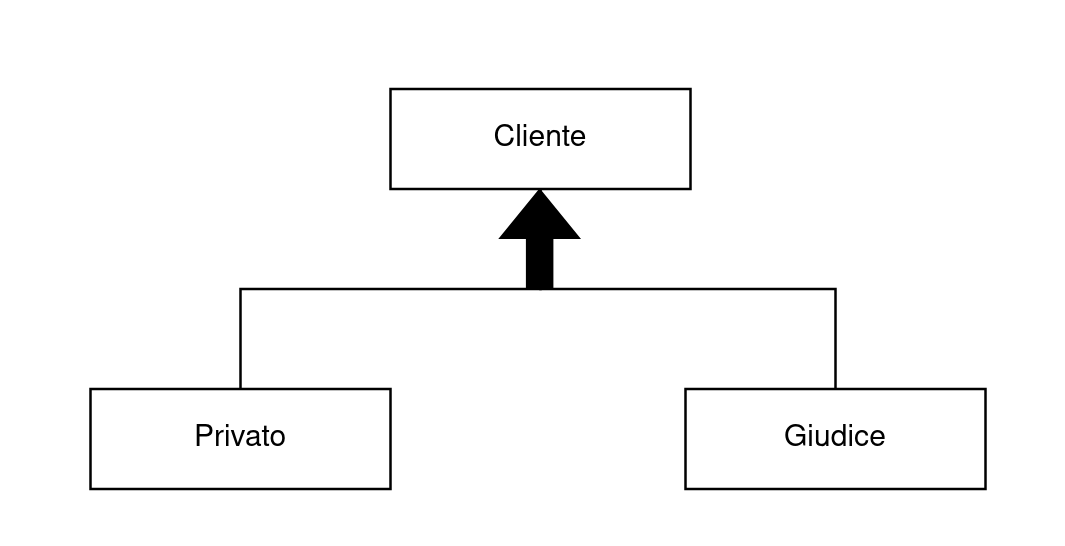
\includegraphics[scale=0.4]{../Img/DBSchemes/cliente-1.png} 
            \end{figure}
            
            Questa prima specializzazione é nata dall'idea che i clienti, in generale, potevano essere, appunto, di due tipi distinti:\\
            I \textbf{Giudici} sono un tipo particolare di cliente che può richiedere una \textit{consulenza tecnica} allo studio. Infatti, generalmente, le consulenze tecniche sono richieste
            dai giudici e non da privati o altre imprese.\\
            I \textbf{Privati}, invece, sono tutti gli altri tipi di cliente.\\

            In principio, c'era anche l'idea di specializzare \textbf{Clienti} in \textbf{Pubblico} e \textbf{Privato}, però, parlandone con i tecnici dello studio, abbiamo concluso che questa suddivisione
            era eccessiva poiché gli unici clienti che potevano essere categorizzati come \textit{pubblici} erano, appunto, i giudici.

            Proseguendo con la strategia top-down, abbiamo specializzato \textbf{Privato} in:\\
            \textbf{Persona fisica}: persone che hanno richiesto una prestazione allo studio..
            \textbf{Condominio}: condomini che hanno richiesto una prestazione allo studio.
            \textbf{Impresa}: imprese che hanno richiesto una prestazione allo studio.

            \begin{figure}[H]
                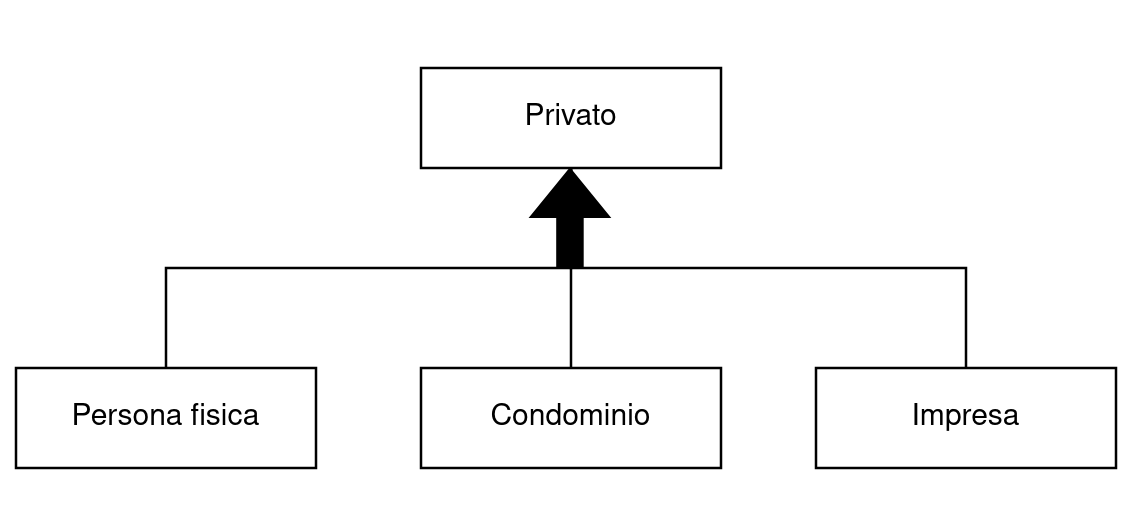
\includegraphics[scale=0.4]{../Img/DBSchemes/cliente-2.png}
            \end{figure}
        
            \newpage
            Lo schema ottenuto é il seguente:

            \begin{figure}[H]
                \makebox[\textwidth]{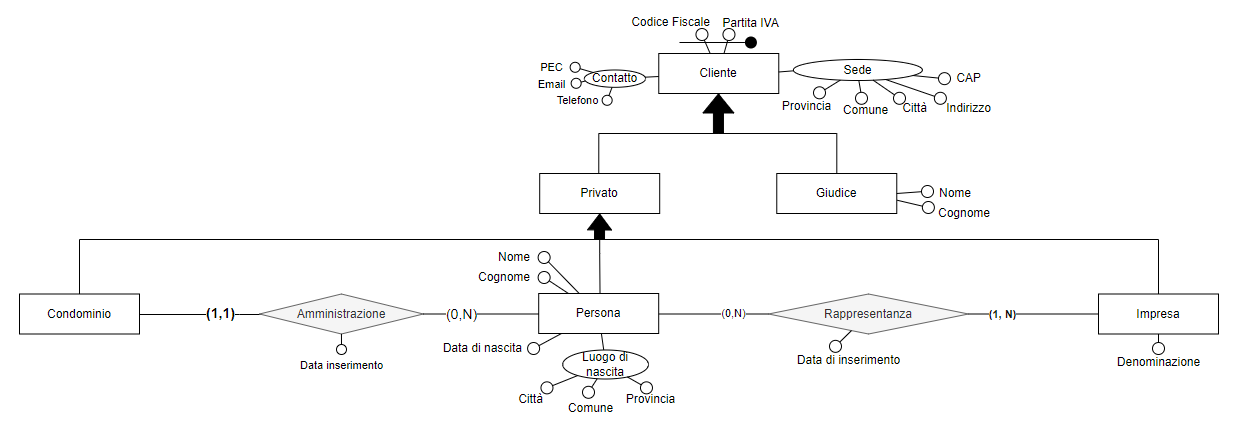
\includegraphics[scale=0.6]{../Img/DBSchemes/cliente-3.png}}
            \end{figure}

            Da questo risultato abbiamo potuto notare che alcuni attributi tra \textit{Cliente, Giudice e Persona} erano simili ed in parte ridondanti. Abbiamo perciò deciso di integrare \textit{Giudice} in \textit{Persona},
            eliminando perciò la generalizzazione \textit{Privato}.
            Abbiamo inoltre aggiunto due relazioni:
            \textbf{Amministrazione}: mette in relazione un condominio con una persona fisica che rappresenta l'amministratore di condominio.
            \textbf{Rappresentanza}: mette in relazione un impresa con una persona fisica che rappresenta il suo rappresentante legale.
            Queste relazioni implicano che se un condominio o un'impresa richiedono una prestazione allo studio diverranno clienti anche l'amministratore del primo e il rappresentante della seconda, risultando coerente con la metodologia di lavoro dello studio.
            Le due relazioni contengono anche l'attributo "Data Inserimento", che permette quindi di avere uno storico, prendendo come attuale amministratore o rappresentante l'istanza con la data più recente. Riteniamo pertanto che questo ciclo non rappresenti una ridondanza.

            \begin{figure}[H]
                \makebox[\textwidth]{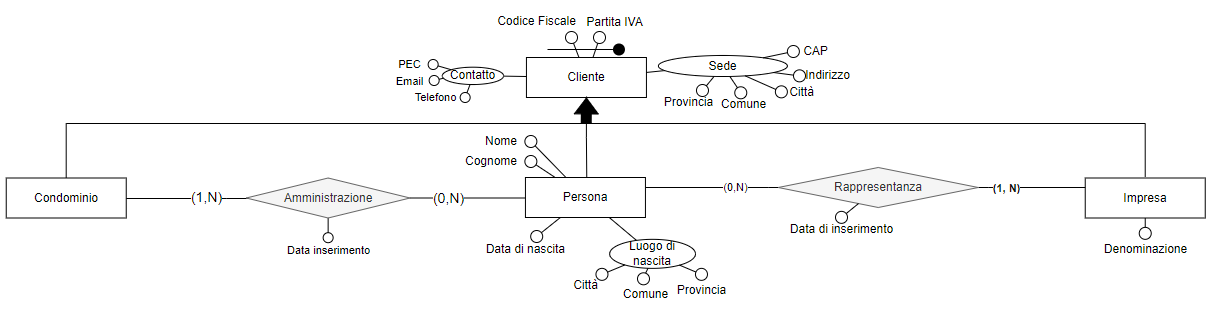
\includegraphics[scale=0.6]{../Img/DBSchemes/cliente-ristrutturato.png}}
                \caption{Schema parziale sviluppato partendo da Cliente}
            \end{figure}

            \subsection{Tecnico}
            Per quanto riguarda l'entità \textbf{Tecnico} abbiamo aggiunto l'entità \textbf{Attestato} poiché è necessario tener conto degli attestati perseguiti dai tecnici dello studio. Inoltre inserito 3 relazioni con Lavoro con significati diversi:
            \textbf{Partecipazione} indica i tecnici che hanno preso parte ad un lavoro;
            \textbf{Supervisione} indica il tecnico legalmente responsabile per un lavoro;
            \textbf{Direzione} indica il tecnico che si occupa della direzione dei lavori del cantiere nel caso sia affidata allo studio.
            
            \begin{figure}[H]
            	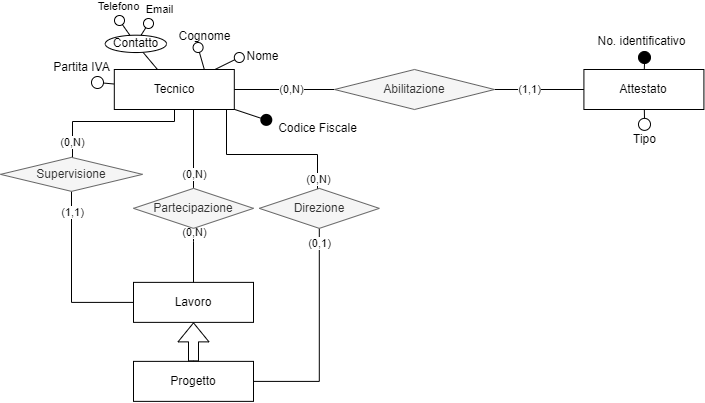
\includegraphics[scale=0.7]{../Img/DBSchemes/tecnico-completo.png} 
                \caption{Schema parziale sviulppato partendo da Tecnico}
            \end{figure}
            
            
            \subsection{Struttura}
            
            Abbiamo inserito due attributi nella relazione \textbf{Proprietà}: \textit{Data inizio proprietà} e \textit{Data fine proprietà}. Questi servono a tenere traccia di chi era il proprietario di una struttura in un determinato periodo.
            Da notare che queste date potrebbero non corrispondere esattamente alle effettive date di inizio e fine proprietà, ma, in generale, corrispondono alle date di inserimento e di modifica della relazione.
            
            \begin{figure}[H]
            	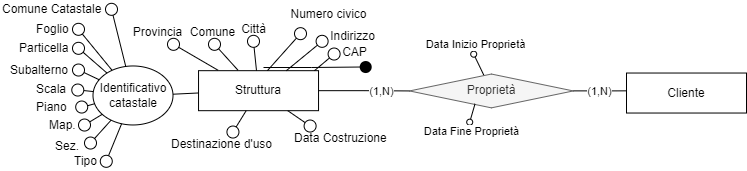
\includegraphics[scale=0.7]{../Img/DBSchemes/struttura-completo.png} 
                \caption{Schema parziale sviluppato partendo da Struttura}
            \end{figure}
            
            
        
	\section{Integrazione schema concettuale}
        A questo punto ci é sorto un dubbio: dobbiamo tenere conto dei tecnici che lavorano ad un progetto?
        Rileggendo nuovamente le interviste, si evince che lo studio non é solito a tenere traccia di chi fa cosa, poiché di
        solito tutti partecipano un pò a tutto. Abbiamo quindi constato che una relazione tra Tecnico e Lavoro risulterebbe
        di intralcio allo Studio, che non é abituato a registrare questa informazione, oltre che a non averne proprio
        bisogno, se non in pochi casi prettamente specifici, ovvero nei lavori di Consulenze.  

        Notare che abbiamo introdotto una nuova simbologia, non presente negli schemi E-R tradizionali, per semplificare la lettura dello schema d'insieme, che indica a
        quale relazione si vanno a collegare 3 delle relazioni di cliente.
        
        \begin{sidewaysfigure}
            \centering
            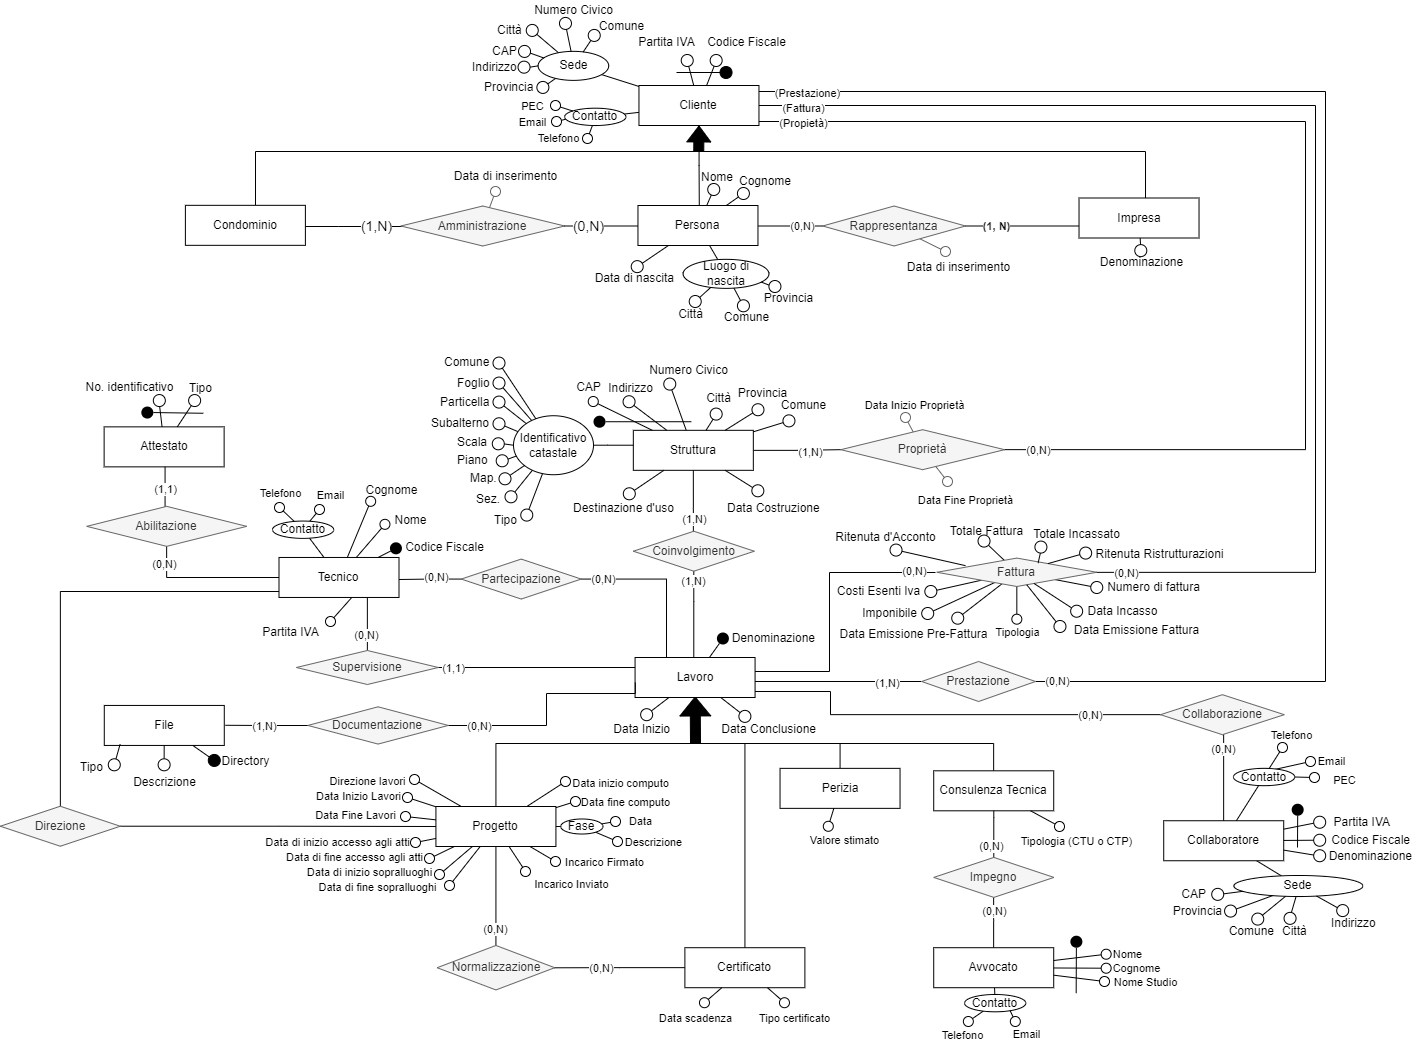
\includegraphics[scale=0.5]{../Img/DBSchemes/schema-concettuale.png}
            \caption{Schema concettuale integrato con strategia bottom-up}
        \end{sidewaysfigure}
        \newpage
	\section{Analisi qualità schema ER}
        \subsection{Correttezza}
        Lo schema rispetta propriamente i costrutti dello schema E-R. Per tanto, non ci sono correzzioni da effettuare. 
        \subsection{Completezza}
        Analizzando la Completezza dello schema, ci siamo resi conto della mancanza di alcuni requisiti espressi inizialmente, ovvero:
        \begin{itemize}
            \item \textbf{Attributo Tipo nell'entità Struttura}: é una descrizione del tipo della struttura. 
            \item \textbf{Attributo Tipo nell'entità Lavoro}: abbiamo deciso rinominare questo attributo in \textbf{Descrizione} poiché soddisfa comunque le stesse esigenze.
            \item \textbf{Attributo Tipo nell'entità Progetto}: indica se il progetto é di tipo "nuovo" o "vecchio".
            \item \textbf{Attributo Lavoro Svolto nella relazione Collaborazione}: serve a sintetizzare l'incarico dell'azienda collaboratrice ad un \textbf{Lavoro}.
            \item \textbf{Attributo Modalità di pagamento nella relazione Fatture}: indica la modalità di pagamento della fattura.
        \end{itemize}
        \subsection{Leggibilità}
        Lo schema ha subito dei cambiamenti grafici per poter permettere una migliore leggibilità dello schema.
        %TODO: SCRIVERE QUALI CAMBIAMENTI, E FARE SCHEMA POST ANALISI BELLO LEGGIBILE
        \subsection{Minimalità}
        Analizzando lo schema abbiamo trovato un ciclo tra \textbf{Lavoro}, \textbf{Struttura} e \textbf{Cliente}: il ciclo
        trovato coinvolge le relazioni \textbf{Prestazione}, \textbf{Coinvolgimento}, e \textbf{Proprietà}; non consideriamo la
        relazione \textbf{Fattura} in questa analisi poiché risulta evidentemente necessaria per poter tenere conto delle fatture
        relative ad un lavoro, e non rappresenta di fatto una relazione adatta a indicare il cliente di un lavoro.
        
        Per poter rimuovere il ciclo dovremmo eliminare la relazione \textbf{Proprietà} o la relazione \textbf{Prestazione}, ma riteniamo
        che debbano essere entrambe presenti, poiché il cliente che richiede il lavoro può non essere proprietario della struttura, come
        ad esempio nel caso di prestazioni richieste da amministratori di condominio, o rappresentanti legali di un impresa; d'altra parte
        la relazione \textbf{Proprietà} è necessaria poiché lo studio deve conoscere tutti i proprietari di una struttura, e permette di
        avere uno storico dei proprietari di un immobile.

        Abbiamo poi notato che alcuni attributi delle specializzazioni di cliente erano in comune con tutte le specializzazioni:
        per questo motivo abbiamo deciso di raggrupparle su \textbf{Cliente}.

        L'attributo \textbf{Totale fattura}, invece, é direttamente derivabile dall'attributo \textbf{Imponibile}, facendo i dovuti calcoli.
        \begin{sidewaysfigure}
            \includegraphics[scale=0.5]{../Img/DBSchemes/post-analisi-qualità.png} 
            \caption{Schema Concettuale finale}
        \end{sidewaysfigure}
        \newpage
	\section{Dizionario dei dati}
	\subsubsection{Entità}
	\begin{longtable}{|p{2cm}|p{4.6cm}|p{6.2cm}|p{3.2cm}|}
            \hline
            \textbf{Entità} & \textbf{Descrizione} & \textbf{Attributi} & \textbf{Identificatore}\\
            \hline
            Lavoro 
		& Generico servizio offerto dallo studio. 
		& Denominazione(Stringa) 
		\newline Data inizio(Data) 
		\newline Data conclusione (Data) 
		\newline Descrizione(Stringa) 
		& Denominazione \\
            \hline
            Progetto  
		& Lavoro che prevede una fase di progettazione. 
		& Direzione lavori(Booleano) 
		\newline Tipo(Stringa)("Nuovo", "Vecchio") 
		\newline Data di inizio accesso agli atti(Data) 
		\newline Data di fine accesso agli atti(Data) 
		\newline Data di inizio sopralluoghi(Data) 
		\newline Data di fine sopralluoghi(Data) 
		\newline Incarico inviato (Data) 
		\newline Incarico Firmato (Data) 
		\newline Fase: 
		\newline - Data(Data) 
		\newline - Descrizione(Stringa) 
		\newline Data inizio computo (Data) 
		\newline Data fine computo(Data) 
		& '' \\
            \hline
            Certificato 
		& Progetto volto al certificare che una struttura rispetti determinati standard. 
		& Tipo certificato(Stringa) 
		\newline Data scadenza(Data) 
		\newline 
		& ''\\
            \hline
            Perizia 
		& Consulenza nella quale si stima il valore di una struttura. 
		& Valore stimato(Numerico) 
		&  '' \\
            \hline
            Consulenza Tecnica 
		& Consulenza svolta in una causa legale. 
		& Tipologia(Stringa)("CTU", "CTP") 
		&  ''\\
            \hline
            Tecnico 
		& Tecnico dello studio. 
		& Nome(Stringa) 
		\newline Cognome(Stringa) 
		\newline Codice fiscale(Stringa) 
		\newline Partita IVA(Numerico) 
		\newline Contatto: 
		\newline - Telefono(Numerico) 
		\newline - Email(Stringa) 
		\newline 
		& Codice fiscale \\
            \hline
            Attestato 
		& Attestato che certifica che un tecnico può svolgere un determinato tipo di lavoro. 
		& Numero identificativo(Stringa) 
		\newline Tipo abilitazione(Stringa) 
		& Numero identificativo \\
            \hline
            Avvocato 
		& Avvocato coinvolto in una Consulenza Tecnica. 
		& Nome(Stringa) 
		\newline Cognome(Stringa) 
		\newline Telefono(Stringa) 
		\newline Email(Stringa)
		& Nome 
		\newline Cognome 
		\newline Telefono \\
            \hline
            File 
		& File relativo ad un lavoro. 
		& Descrizione(Stringa) 
		\newline Tipo(Stringa) 
		\newline Directory(Stringa)
		& Directory \\
            \hline
            Collaboratore 
		& Impresa con cui lo studio collabora per un lavoro. 
		& Denominazione(Stringa) 
		\newline Codice Fiscale(Stringa) 
		\newline Partita IVA(Numerico) 
		\newline Email(Stringa) 
		\newline Telefono(Stringa) 
		\newline Sede (CAP, Provincia, Comune, Città, Indirizzo) 
		& Partita IVA 
		\newline Codice fiscale \\
            \hline
            Struttura 
		& Edificio, Immobile. 
		& CAP(Numerico)
		\newline Indrizzo(Stringa)
		\newline Numero Civico(Stringa)
		\newline Città(Stringa) 
		\newline Provincia(Stringa) 
		\newline Comune(Stringa) 
		\newline Identificativo catastale:
                \newline -Comune(Stringa)
                \newline -Foglio(Stringa)
                \newline -Particella(Numerico)
                \newline -Subalterno(Stringa)
                \newline -Scala(Stringa)
                \newline -Piano(Stringa)
                \newline -Sezione(Stringa)
                \newline -Tipo(Stringa)
                \newline Tipo(Stringa)
		\newline Data Costruzione(Data) 
		\newline Destinazione d'uso(Stringa)
		& CAP 
		\newline Indrizzo 
		\newline Numero Civico\\
            \hline
            Cliente 
		& Privato o giudice che richiede un servizio allo studio. 
		& Codice fiscale(Stringa) 
                \newline Partita IVA
                \newline Sede:
		\newline -Numero Civico(Stringa) 
		\newline -Comune(Stringa) 
		\newline -CAP(Numerico) 
		\newline -Indirizzo(Stringa) 
		\newline -Provincia(Stringa) 
		\newline -Città(Stringa) 
                \newline Contatto:
                \newline -Telefono(Numerico)
                \newline -Email(Stringa)
                \newline -PEC(Stringa):
                
		& Codice fiscale \\
            \hline
            Persona 
		& Persona fisica cliente dello studio. 
		& Nome(Stringa) 
		\newline Cognome(Stringa) 
		\newline Data di nascita(Data) 
		\newline Luogo di nascita: 
		\newline - Comune(Stringa) 
		\newline - Città(Stringa) 
		\newline - Provincia(Stringa) 
		& ''\\
            \hline
            Condominio 
		& Condominio cliente dello studio. 
		& ''
		& ''\\
            \hline
            Impresa 
		& Società cliente dello studio. 
		& Denominazione(Stringa) 
		& ''\\
            \hline
            \caption{Dizionario delle entità}
	\end{longtable}
	\newpage
	\subsubsection{Relazioni}
	\begin{longtable}{|p{2.5cm}|p{5cm}|p{3.8cm}|p{4.7cm}|}
            \hline
            \textbf{Relazione} & \textbf{Descrizione} & \textbf{Entità coinvolte} & \textbf{Attributi}\\
            \hline
            Partecipazione
		& Associa ad un lavoro i tecnici coinvolti.
		& Lavoro(0,N) 
		\newline Tecnico(0,N) 
		& ***\\
            \hline
            Supervisione
		& Associa ad un lavoro il tecnico legalmente responsabile.
		& Lavoro(1,1) 
		\newline Tecnico(0,N)
		& ***\\
            \hline
            Direzione 
		& Associa ad una lavoro nel quale si effettua la direzione lavori il tecnico che se ne occupa. 
		& Progetto(0,1) 
		\newline Tecnico(0.N)
		&\\
            \hline
            Abilitazione 
		& Associa ad un tecnico gli attestati che ha conseguito. 
		& Tecnico(0,N) 
		\newline Attestato(1,1) 
		& ***\\
            \hline
            Normalizzazione
		& Associa ad un lavoro di certificazione i progetti coinvolti.
		& Certificazione(0,N) 
		\newline Progetto(0,N) 
		& ***\\
            \hline
            Documentazione 
		& Associa ad un lavoro i File che lo riguardano. 
		& Lavoro(0,N) 
		\newline File(1,N)
		&***\\
            \hline
            Impegno
		& Associa ad una consulenza tecnica gli avvocati coinvolti.
		& Consulenza Tecnica(0.N) 
		\newline Avvocato(0,N) 
		& ***\\
            \hline
            Collaborazione
		& Associa ad un lavoro i collaboratori coinvolti.
		& Lavoro(0,N) 
		\newline Collaboratore(0,N) 
                & Lavoro Svolto(Stringa)\\
            \hline
            Coinvolgimento
		& Associa ad un lavoro le strutture coinvolte.
		& Lavoro(1,N) 
		\newline Strutture(0,N) 
		& ***\\
            \hline
            Proprietà
		& Associa ad una struttura i clienti che la possiedono.
		& Struttura(1,N) 
		\newline Cliente(0,N) 
                & Data inizio proprietà(Data),
                Data Fine proprietà(Data)\\
            \hline
            Fattura
		& Associa ad un lavoro i clienti a cui è stata mandata una fattura.
		& Lavoro(0,N) 
		\newline Cliente(0,N) 
                & Numero di fattura(Numerico),
                 Modalità(Stringa),
                 Imponibile(Numerico),
                 Costi esenti IVA(Numerico),
                 Ritenuta d'acconto(Numerico),
                 Ritenuta ristrutturazioni(Numerico),
                 Data Emissione Pre-Fattura(Data),
                 Data Emissione Fattura(Data),
                 Data Incasso(Data)
                 Tipologia(Stringa) \\
            \hline
            Prestazione
		& Associa ad un lavoro i clienti a cui viene fornita la prestazione 
		& Lavoro(1,N) 
		\newline Cliente(0,N) 
		& ***\\
            \hline
            Amministrazione
		& Associa ad un condominio il suo amministratore.
		& Condominio(1,N) 
		\newline Persona(0,N) 
		& Data inserimento\\
            \hline
            Rappresentanza
		& Associa ad un'impresa il suo rappresentante legale.
		& Impresa(1,N) 
		\newline Persona(0,N)
		& Data inserimento\\
            \hline
            \caption{Dizionario delle relazioni}
	\end{longtable}
        \newpage
	\section{Regole Aziendali}
        \subsection{Regole di Vincolo}
        \begin{enumerate}[label=RV\arabic*]
            \item Le \textit{date di fine} devono essere sempre maggiori delle \textit{date di inizio} che fanno riferimento allo stesso concetto.
            \item Le \textit{date di fine} possono essere aggiornate solo se è presente una \textit{data di inizio} che fa riferimento allo stesso concetto.
            \item Nella relazione \textit{Amministrazione} la \textit{data di inserimento} deve essere maggiore della precedente occerenza.
            \item Nella relazione \textit{Amministrazione} la \textit{data di inserimento} deve essere maggiore della \textit{data di nascita} della \textit{Persona}.
            \item Nella relazione \textit{Rappresentanza} la \textit{data di inserimento} deve essere maggiore della precedente occerenza.
            \item Nella relazione \textit{Rappresentanza} la \textit{data di inserimento} deve essere maggiore della \textit{data di nascita} della \textit{Persona}.
            \item Nella relazione \textit{Propietà} la \textit{data di inizio proprietà} deve essere maggiore o uguale della \textit{data costruzione} della \textit{Struttura}.
            \item Nella relazione \textit{Propietà} la \textit{data di inizio proprietà} deve essere maggiore della \textit{data di nascita} del \textit{Cliente}. 
            \item Nella \textit{Fattura}, la \textit{data di emissione fattura} deve essere maggiore della \textit{data di emissione della pre-fattura}.
            \item Nella \textit{Fattura}, la \textit{data di incasso} deve essere maggiore della \textit{data di emissione fattura}.
            \item In un \textit{Lavoro}, la \textit{data conclusione} deve essere maggiore di tutte le altre date, se presenti, dello stesso lavoro.
            \item Una \textit{Certificazione} può essere eseguita solo da un tecnico che possiede l'\textit{Attestato} necessario.
            \item Un \textit{Tecnico} che è \textit{supervisore} di un \textit{Lavoro} deve \textit{partecipare} allo stesso \textit{Lavoro}.
            \item Un \textit{Tecnico} che è \textit{direttore dei lavori} di un \textit{Lavoro} deve \textit{partecipare} allo stesso \textit{Lavoro}.
            \item L'\textit{incarico} può essere \textit{firmato} solo se è già stato \textit{inviato}.
            \item In \textit{Fattura}, la \textit{ritenuta ristrutturazioni} non può essere aggiornato se il \textit{Lavoro} a quale fa riferimento non è un lavoro di ristrutturaione.
        \end{enumerate}
        \subsection{Regole di Derivazione}
        \label{subsec:derivazioni}
        I seguenti vincoli di derivazione sono stati inseriti comunque anche se gli attributi \textit{Totale Fattura} e \textit{Totale Incassato} sono stati rimossi dalla analisi di qualità, poichè non scartiamo la possibilità
        di reinserirli nel caso in cui, dal calcolo dei costi delle operazioni, risultasse più conveniente mantenere le ridondanze.
        \begin{enumerate}[label=RD\arabic*]
            \item Il \textit{Totale della Fattura} si ottiene seguendo questa formula: Totale fattura = ((imponibile + (4\% dell'imponibile)) + (il 22\% di (imponibile + (4\% dell'imponibile))) + costi esenti iva + ritenuta d'acconto
            \item Il \textit{Totale incassato} si ottiene seguendo questa formual: Totale incassato = Totate fattura - Ritenuta ristrutturazioni
        \end{enumerate}
	\chapter{Progettazione Logica}
	\section{Tavola dei volumi}
        I volumi non hanno tutti un valore \textit{esatto}, poiché i tencici stessi non possiedo una
        informazione certa, pertanto sono stati stimati basandosi su quanto é stato dichiarato da loro e da ipotesi fatte su queste.
        Inoltre, i seguenti volumi sono da riferirsi per un arco di tempo pari a 10 anni, ovvero da quando lo studio ha iniziato a raccogliere i dati in formato digitale.

        
        \textbf{Breve legenda:} \volumeEsatto{Volume Esatto} ; \volumeCalcolato{Volume Calcolato}
        \begin{longtable}{|p{7cm}|c|p{7cm}|}
		\hline
		\textbf{CONCETTO} & \textbf{TIPO} & \textbf{VOLUME} \\
		\hline
                Lavoro & E & \volumeEsatto{\volumeLavoro} \\
		\hline		
                Progetto & E & \volumeCalcolato\volumeProgetto \\ 
		\hline		
                Certificato & E & \volumeCalcolato\volumeCertificato \\ 
		\hline
		Perizia & E & \volumeCalcolato\volumePerizia \\
		\hline	
		Consulenza Tecnica & E & \volumeCalcolato\volumeConsulenza \\
		\hline
                Tecnico & E & \volumeEsatto\volumeTecnico\\
		\hline
                Attestato & E & \volumeEsatto\volumeAttestato\\
                \hline
                Avvocato & E & \volumeCalcolato\volumeAvvocato \\
		\hline
                File & E & \volumeCalcolato\volumeFile\\
		\hline
                Collaboratore & E & \volumeEsatto\volumeCollaboratore\\
		\hline
                Struttura & E & \volumeEsatto\volumeStruttura \\
		\hline
                Cliente & E & \volumeEsatto\volumeCliente \\
		\hline
		Persona & E & \volumeCalcolato\volumePersona \\
		\hline
		Condominio & E & \volumeCalcolato\volumeCondominio \\
		\hline
		Impresa & E & \volumeCalcolato\volumeImpresa \\
		\hline
		\hline
		Partecipazione & R & \volumeCalcolato\volumePartecipazione \\
                \hline
                Supervisione & R & \volumeCalcolato\volumeSupervisione \\
                \hline
                Direzione & R & \volumeCalcolato\volumeDirezione \\
		\hline
                Abilitazione & R & \volumeCalcolato\volumeAbilitazione \\
                \hline
                Normalizzazione & R & \volumeCalcolato\volumeNormalizzazione\\
		\hline
		Documentazione & R & \volumeCalcolato\volumeDocumentazione \\
		\hline
                Impegno & R & \volumeCalcolato\volumeImpegno \\
		\hline
		Collaborazione & R & \volumeCalcolato\volumeCollaborazione \\
		\hline
		Coinvolgimento & R & \volumeCalcolato\volumeCoinvolgimento \\
		\hline
		Proprietà & R & \volumeCalcolato\volumePropieta \\
		\hline
		Fattura & R & \volumeCalcolato\volumeFattura \\
		\hline
		Prestazione & R & \volumeCalcolato\volumePrestazione \\
		\hline
		Amministrazione & R & \volumeCalcolato\volumeAmministrazione \\
		\hline
		Rappresentanza & R & \volumeCalcolato\volumeRappresentanza \\
		\hline
                \caption{Tavola dei volumi}
	\end{longtable}
        \newpage
	\section{Tavola delle Operazioni}
        \label{sec:tavolaOperazioni}
        La seguente Tavola delle Operazioni riporta una lista completa delle operazioni previste per il database.
        Da notare che il contenuto della tavola è differente da quella presentata in pagina
        ~\pageref{subsec:listOperazioni} poiché questa è stata riadattata alla struttura dello schema finale.
        Anche le frequenze sono cambiate: alcune direttamente grazie al dialogo con lo studio avvenuto 
        successivamente alle interviste formali, altre, invece, hanno un valore stimato basandosi su ipotesi
        fatte in relazione a quanto ci è stato riferito dai tecnici.

        \newcommand{\settimana}[1]{\the\numexpr #1 * 5 \relax}
        \newcommand{\mese}[1]{\the\numexpr\settimana #1 * 4 \relax}
        \newcommand{\anno}[1]{\the\numexpr\mese #1 * 12 \relax}
        \begin{enumerate}[label=Ipotesi \arabic*]
            \item 1 settimana = 5 giorni 
            \item 1 mese = 4 settimane = \mese{1} giorni
            \item 1 anno = 12 mesi = \anno{1} giorni 
        \end{enumerate}

        \newcommand{\convertAnno}[2]{\the\dimexpr #1 / \anno{1} * #2 \relax}
        \newcommand{\convertMese}[2]{\the\dimexpr #1 / \mese{1} * #2 \relax}
        \newcommand{\convertSettimana}[2]{\the\dimexpr #1 / \settimana{1} \relex}
        \begin{longtable}{|p{13cm}|r|}
            \hline
            Aggiornamento Cliente  &  5 al mese \\
            \hline
            Aggiornamento Collaboratore  &  10 all'anno \\
            \hline
            Aggiornamento Fattura  & \fattureMedieMensili al mese \\
            \hline
            Aggiornamento Struttura  & 70 all'anno \\
            \hline
            Aggiornamento di Certificato  & 35 all'anno \\
            \hline
            Aggiornamento di Consulenza Tecnica  & 48 all'anno \\
            \hline
            Aggiornamento di Perizia di Stima  & 20 all'anno \\
            \hline
            Aggiornamento di Lavoro, data di conclusione  & 100 all'anno \\
            \hline
            Aggiornamento di Progetto, data di fine accesso agli atti  & 100 all'anno \\
            \hline
            Aggiornamento di Progetto, data di fine computo  & 95 all'anno \\
            \hline
            Aggiornamento di Progetto, data di fine lavori  & 100 all'anno \\
            \hline
            Aggiornamento di Progetto, data di fine sopralluoghi  & 100 all'anno \\
            \hline
            Aggiornamento di Progetto, data di inizio accesso agli atti  & 100 all'anno \\
            \hline
            Aggiornamento di Progetto, data di inizio computo  & 95 all'anno \\
            \hline
            Aggiornamento di Progetto, data di inizio lavori  & 100 all'anno \\
            \hline
            Aggiornamento di Progetto, data di inizio sopralluoghi  & 100 all'anno \\
            \hline                    
            Aggiunta Partecipazione di Tecnico a Lavoro  & 200 all'anno \\
            \hline
            Aggiunta di Amministratore di un condominio  &  20 all'anno \\
            \hline
            Aggiunta di Coinvolgimento di una nuova struttura a progetto  &  1 all'anno \\
            \hline
            Aggiunta di Collaborazione a progetto  & 80 all'anno \\
            \hline
            Aggiunta di Fattura  & 80 all'anno \\
            \hline
            Aggiunta di Impegno avvocato a consulenza tecnica  &  8 al mese \\
            \hline 
            Aggiunta di Proprietario di struttura  & 5 all'anno \\
            \hline
            Aggiunta di Raprresentanza di un'impresa  & 10 all'anno \\
            \hline
            Calcolo Numero di lavori a cui ha partecipato un tecnico in un anno categorizzandoli per tipo  & 5 all'anno \\
            \hline
            Cancellazione Cliente &  1 volta all'anno \\ %solo se non è mai stato coinvolto in un lavoro o se non posside una struttura   
            \hline
            Cancellazione Collaborazione  &  5 all'anno \\
            \hline 
            Cancellazione Lavoro  &  10 all'anno \\ % solo se senza fattura 
            \hline
            Concludi Lavoro  & 80 all'anno \\
            \hline
            Consultazione Attestati di un Tecnico  &  10 all'anno \\
            \hline
            Consultazione Avvocato  & 20 all'anno \\
            \hline
            Consultazione Cliente  & 5 al giorno \\
            \hline
            Consultazione Collaboratore  & 20 al mese \\
            \hline
            Consultazione Collaboratori che hanno lavorato in una Struttura  & 20 all'anno \\
            \hline
            Consultazione Fatture di un Cliente  &  10 al mese \\
            \hline
            Consultazione Fatture di un Lavoro  & 10 volte mese \\
            \hline
            Consultazione File relativi ad un Lavoro  & 20 al mese \\
            \hline
            Consultazione Lavori conclusi  & 5 al mese \\
            \hline
            Consultazione Lavori di un Cliente  &  10 mese \\
            \hline
            Consultazione Lavori in Corso  & 50 al giorno \\
            \hline
            Consultazione Lavori in un Luogo & 20 all'anno \\
            \hline
            Consultazione Lavori relativi ad una Struttura  & 3 al mese \\
            \hline
            Consultazione Lavoro  & 30 al giorno \\
            \hline
            Consultazione Struttura  & 5 al giorno \\
            \hline
            Consultazione Tecnico  & 2 al mese \\
            \hline 
            Consultazione Totale Fattura di una Fattura  & 20 al mese \\
            \hline
            Consultazione Totale Incassato in un anno, partendo dall'inizio dell'anno corrente  & 50 all'anno \\
            \hline
            Consultazione Totale Incassato per tipologia di lavoro  & 4 all'anno \\
            \hline
            Consultazione Totale Incassato per un lavoro  & 4 al mese \\
            \hline
            Consultazione Totale Fatturato in un anno, partendo dall'inizio dell'anno corrente  & 50 all'anno \\
            \hline
            Inserimento di Attestato  &  1 all'anno \\
            \hline 
            Inserimento di Avvocato  &  8 al mese \\
            \hline
            Inserimento di Cliente  & \the\numexpr \volumeCliente / 10 \relax all'anno \\
            \hline
            Inserimento di Collaboratore  &  20 all'anno \\
            \hline
            Inserimento di File  & 20 al giorno \\
            \hline 
            Inserimento di Lavoro  & \the\numexpr \volumeLavoro / 10 \relax all'anno \\
            \hline
            Inserimento di Struttura  & 80 all'anno \\
            \hline
            Inserimento di Tecnico  &  3 all'anno \\
            \hline
            Modifica Avvocato, Email e Telefono  &  5 all'anno \\
            \hline
            Modifica Denominazione di un Lavoro  &  10 all'anno \\
            \hline
            Modifica Perizia, Valore Stimato  &  5 all'anno \\
            \hline
            Modifica Persona, Dati di residenza, Numero di telefono e email  &  10 all'anno \\
            \hline
            Modifica Progetto, Direzione Lavori  &  15 all'anno \\
            \hline
            Modifica Tecnico, Telefono e Email  &  2 all'anno \\
            \hline
            Ricerca Condominio per composizione di Comune, Provincia, Città, Indirizzo, CAP e numero Civico  &  10 al mese \\
            \hline
            Ricerca Fatture non incassate  & 20 all'anno \\
            \hline
            Ricerca Impresa per Denominazione  & 30 al mese \\
            \hline
            Ricerca Impresa per Rappresentante  & 10 al mese \\
            \hline
            Ricerca Lavori per Denominazione  & 30 al giorno \\
            \hline
            Ricerca Lavori svolti in un periodo di tempo  & 10 all'anno \\
            \hline
            Ricerca Lavori svolti per luogo  & 20 all'anno \\
            \hline 
            Ricerca Persona per Nome e Cognome  & 30 al mese \\
            \hline
            Ricerca Strutture che hanno delle certificazioni in scadenza in questo anno  & 20 all'anno \\
            \hline
            Statistica dei clienti per cui sono stati effettuati più lavori in un determinato periodo di tempo  & 20 all'anno \\
            \hline
            Statistica dei collaboratori che hanno partecipato più spesso ai lavori dello Studio categorizzandoli per il tipo di lavoro svolto  & 20 all'anno \\
            \hline
            Statistica dei comuni per cui sono stati svolti più lavori raggruppandoli per tipo di lavoro  & 20 all'anno \\
            \hline
        \end{longtable}


        \newpage
	\section{Ristrutturazione Schema Concettuale}
        In questa fase ci occuperemo di ottimizzare lo schema secondo alcuni criteri standard per semplificare le fasi successive della progettazione.
        Consideriamo che una operazione di scrittura equivale a due operazioni di lettura (1S = 2L) in termini di richiesta computazionale.

	\subsection{Analisi Derivazioni e Ridondanze}
        Analizzando la tavola delle operazioni, tenendo conto anche delle ridondanze già individuate, abbiamo individuato le seguenti come possibili ridondanze da inserire
        al fine di ottimizzare il costo delle operazioni:

        \begin{itemize}
            \item Totale fattura su Fattura, fa riferimento alla ridondanza RD1, discussa a pagina \pageref{subsec:derivazioni}
            \item Totale incassato su Fattura, fa riferimento alla ridondanza RD2, discussa a pagina \pageref{subsec:derivazioni}.
            \item Totale incassatto su Lavoro, ovvero un attributo calcolato che indica quanto è stato incassato da quel lavoro.
            \item Totale Fatturato su Lavoro, ovvero un attributo calcolato che indica quanto è stato incassato da quel lavoro. 
        \end{itemize}
        Abbiamo inoltre trovato altri possibili candidati che però abbiamo scartato poiché lo studio risulta essere
        uno sforzo eccessivo per un guadagno trascurabile, come, ad esempio:
        \begin{itemize}
            \item Attributo che indica il numero di lavori svolti da un tecnico in un anno: l'unica operazione
                che necessita di questa informazione è la OpCon 28 che viene eseguita 5 volte all'anno.
            \item Attributo che indica il luogo di un lavoro.
        \end{itemize}
        Nelle seguenti analisi, valgono le ipotesi fatte nella sezione~\nameref{sec:tavolaOperazioni} a pagina \pageref{sec:tavolaOperazioni}.

        Inoltre, il calcolo di "Totale Fatturato" e "Totale Incassato" è indipendente l'uno dall'altro, poichè, nel calcolo dei due attributi,
        consideriamo solo i valori atomici necessari per effettuare il calcolo.
        
        % +++++++++++++++++++++++++++++++++INIZIO PRIMO STUDIO+++++++++++++++++++++++++++++
        \subsection{Attributo: "Totale fattura" in "Fattura"}
        Premessa: Abbiamo convertito le frequenze ad una unità di misura univoca, ovvero numero di operazioni al \textit{mese}, in maniera tale da facilitare il calcolo del costo delle operazioni.
        L'inserimento di questa ridondanza è stata presa in considerazione poiché per lo studio è interessante,
        e richiesto, consultare il totale di una fattura. Infatti, le operazioni che richiedono questa informazione sono:
        \begin{itemize}
            \item Opta 1 Aggiunta di Fattura (7 al mese)
            \item Opta 2 Consultazione delle fatture di un cliente (10 al mese)
            \item Opta 3 Consultazione delle Fatture di un Lavoro (10 al mese)
            \item Opta 4 Consultazione Totale Fatturato di una fattura (20 al mese)
            \item Opta 5 Consultazione Totale Fatturato delle fatture emesse in un anno (4 al mese)
        \end{itemize}
        Tuttavia, l'unica operazione discriminante é la Opta 1 poichè per le consultazioni il numero degli
        accessi è invariato.
        \newcommand\optaOne{7}
        \paragraph{Presenza di ridondanza}
        \begin{table}[H]
            \begin{tabular}{|p{5cm}|c|c|p{5cm}|}
            \hline
            \multicolumn{4}{|c|}{Operazione Opta 1}\\ 
            \hline
            \textbf{CONCETTO} & \textbf{COSTRUTTO} & \textbf{ACCESSI} & \textbf{TIPO} \\
            \hline
                Fattura & Relazione & 2 & S \\
            \hline
            \end{tabular}
        \end{table}
        \paragraph{Assenza di ridondanza}
        \begin{table}[H]
            \begin{tabular}{|p{5cm}|c|c|p{5cm}|}
            \hline
            \multicolumn{4}{|c|}{Operazione Opta 1: \frequenzaOpAdd}\\ 
            \hline
            \textbf{CONCETTO} & \textbf{COSTRUTTO} & \textbf{ACCESSI} & \textbf{TIPO} \\
            \hline
            Fattura & Entità & 1 & S \\
            \hline
            \end{tabular}
        \end{table}

        \paragraph{Cost Totali}        
        \begin{longtable}{|p{4cm}|p{4cm}|p{4cm}|p{4cm}|}
            \hline
            \multicolumn{4}{|c|}{Costo totale con ridondanza} \\ 
            \hline
            \textbf{Operazione} & \textbf{Costo} & \textbf{Frequenza mensile} & \textbf{Totale} \\
            \hline
                Opta 1 &
                2S = 4L &
                \optaOne &
                \the\numexpr \optaOne * 4 \relax \\
            \hline
            \hline
                \multicolumn{3}{|r|}{Totale con ridondanza} &
                \the\numexpr 
                (\optaOne * 4)
                \relax \\ 
            \hline
        \end{longtable} 
        \begin{longtable}{|p{4cm}|p{4cm}|p{4cm}|p{4cm}|}
            \hline
            \multicolumn{4}{|c|}{Costo totale senza ridondanza} \\ 
            \hline
            \textbf{Operazione} & \textbf{Costo} & \textbf{Frequenza mensile} & \textbf{Totale} \\
            \hline
                Opta 1 &
                1S = 2L &
                \optaOne &
                \the\numexpr \optaOne * 2 \relax \\
            \hline
            \hline
                \multicolumn{3}{|r|}{Totale con ridondanza} &
                \the\numexpr 
                (\optaOne * 2)
                \relax \\ 
            \hline
        \end{longtable} 
        Dal risultato ottenuto, è più conveniente non inserire la ridondanza.
        % +++++++++++++++++++++++++++++++++FINE PRIMO STUDIO+++++++++++++++++++++++++++++

        \subsection{Attributo: "Totale Incassato" in "Fattura"}
        Dal precedente risultato è immediato anche il risultato di questo studio. Per tanto,
        conviene non inserire la ridondanza.

        % +++++++++++++++++++++++++++++++INIZIO SECONDO STUDIO+++++++++++++++++++++++++++
        \subsection{Attributo "Totale Incassato" su "Lavoro"}
        Le operazioni coinvolte sono le seguenti:
        \begin{itemize}
            \item  Opti 1 Aggiunta di Fattura (80 all'anno)
            \item  Opti 2 Consultazione Totale Incassato in un anno (50 all'anno)
            \item  Opti 3 Consultazione Totale Incassato per tipologia di lavoro (4 all'anno)
            \item  Opti 4 Consultazione Totale Incassato per un lavoro (50 all'anno)
        \end{itemize}
        \newcommand\optiOne{80}
        \newcommand\optiTwo{50}
        \newcommand\optiThree{4}
        \newcommand\optiFour{50}
        \newcommand\lavoriMediMensili{\the\numexpr (\volumeLavoro/120) \relax}
        \newcommand\lavoriMediMensiliAnno{\the\numexpr (\lavoriMediMensili*13)/2 \relax}
        \newcommand\fattureMedieMensiliAnno{\the\numexpr (\fattureMedieMensili*13)/2 \relax }

        \paragraph{Assenza di Ridondanza}

        \begin{table}[H]
            \begin{tabular}{|p{5cm}|c|c|p{5cm}|}
            \hline
            \multicolumn{4}{|c|}{Operazione Opti 1}\\ 
            \hline
            \textbf{CONCETTO} & \textbf{COSTRUTTO} & \textbf{ACCESSI} & \textbf{TIPO} \\
            \hline
            Fattura & Relazione & 1 & S \\
            \hline
            \end{tabular}
        \end{table}

        \begin{table}[H]
            \begin{tabular}{|p{5cm}|c|c|p{5cm}|}
            \hline
            \multicolumn{4}{|c|}{Operazione Opti 2}\\ 
            \hline
            \textbf{CONCETTO} & \textbf{COSTRUTTO} & \textbf{ACCESSI} & \textbf{TIPO} \\
            \hline
                Fattura & Relazione & \fattureMedieMensiliAnno & L \\ 
            \hline
            \end{tabular}
        \end{table}

        \begin{table}[H]
            \begin{tabular}{|p{5cm}|c|c|p{5cm}|}
            \hline
            \multicolumn{4}{|c|}{Operazione Opti 3}\\ 
            \hline
            \textbf{CONCETTO} & \textbf{COSTRUTTO} & \textbf{ACCESSI} & \textbf{TIPO} \\
            \hline
            Lavoro & Entità & \volumeLavoro & L \\
            \hline
            Fattura & Relazione & \volumeFattura & L \\ 
            \hline
            \end{tabular}
        \end{table}

        \begin{table}[H]
            \begin{tabular}{|p{5cm}|c|c|p{5cm}|}
            \hline
            \multicolumn{4}{|c|}{Operazione Opti 4}\\ 
            \hline
            \textbf{CONCETTO} & \textbf{COSTRUTTO} & \textbf{ACCESSI} & \textbf{TIPO} \\
            \hline
            Lavoro & Entità & 1 & L \\
            \hline
            Fatture & Relazione & \fattureMedie & L \\ 
            \hline
            \end{tabular}
        \end{table}

        \paragraph{Presenza di Ridondanza}
        \begin{table}[H]
            \begin{tabular}{|p{5cm}|c|c|p{5cm}|}
            \hline
            \multicolumn{4}{|c|}{Operazione Opti 1}\\ 
            \hline
            \textbf{CONCETTO} & \textbf{COSTRUTTO} & \textbf{ACCESSI} & \textbf{TIPO} \\
            \hline
                Lavoro & E & 1 & S \\
            \hline
                Fattura & R & 1 & S \\
            \hline
            \end{tabular}
        \end{table}

        \begin{table}[H]
            \begin{tabular}{|p{5cm}|c|c|p{5cm}|}
            \hline
            \multicolumn{4}{|c|}{Operazione Opti 2}\\ 
            \hline
            \textbf{CONCETTO} & \textbf{COSTRUTTO} & \textbf{ACCESSI} & \textbf{TIPO} \\
            \hline
                Lavoro & E & \lavoriMediMensiliAnno & L \\
            \hline
            \end{tabular}
        \end{table}
        
        \begin{table}[H]
            \begin{tabular}{|p{5cm}|c|c|p{5cm}|}
            \hline
            \multicolumn{4}{|c|}{Operazione Opti 3}\\ 
            \hline
            \textbf{CONCETTO} & \textbf{COSTRUTTO} & \textbf{ACCESSI} & \textbf{TIPO} \\
            \hline
                Lavoro & Entità & \volumeLavoro & L \\
            \hline
            \end{tabular}
        \end{table}

        \begin{table}[H]
            \begin{tabular}{|p{5cm}|c|c|p{5cm}|}
            \hline
            \multicolumn{4}{|c|}{Operazione Opti 4}\\ 
            \hline
            \textbf{CONCETTO} & \textbf{COSTRUTTO} & \textbf{ACCESSI} & \textbf{TIPO} \\
            \hline
                Lavoro & Entità & 1 & L \\ 
            \hline
            \end{tabular}
        \end{table}
        
        
        \paragraph{Costi Totali} 
        \begin{longtable}{|p{4cm}|p{4cm}|p{4cm}|p{4cm}|}
            \hline
            \multicolumn{4}{|c|}{Costo totale senza ridondanza} \\ 
            \hline
            \textbf{Operazione} & \textbf{Costo} & \textbf{Frequenza mensile} & \textbf{Totale} \\
            \hline
                Opti 1 &
                1S = 2L &
                \optiOne &
                \the\numexpr \optiOne * 2 \relax \\
            \hline
                Opti 2 &
                \fattureMedieMensiliAnno L &
                \optiTwo &
                \the\numexpr \optiTwo * \fattureMedieMensiliAnno \relax \\
            \hline
                Opti 3 &
                \the\numexpr \volumeLavoro + \volumeFattura \relax L &
                \optiThree &
                \the\numexpr \optiThree * (\volumeLavoro + \volumeFattura) \relax \\
            \hline
                Opti 4 &
                \the\numexpr 1 + \fattureMedie \relax L &
                \optiFour &
                \the\numexpr \optiFour * (1 + \fattureMedie ) \relax \\
            \hline
                \multicolumn{3}{|r|}{Totale senza ridondanza} &
                \the\numexpr 
                (\optiOne * 2) +
                (\optiTwo * \fattureMedieMensiliAnno ) +
                (\optiThree * (\volumeLavoro + \volumeFattura) ) +
                (\optiFour * (1 + \fattureMedie ) )
                \relax \\ 
            \hline
        \end{longtable}
        \vspace{2cm}
        \begin{longtable}{|p{4cm}|p{4cm}|p{4cm}|p{4cm}|}
            \hline
            \multicolumn{4}{|c|}{Costo totale con ridondanza} \\ 
            \hline
            \textbf{Operazione} & \textbf{Costo} & \textbf{Frequenza mensile} & \textbf{Totale} \\
            \hline
                Opti 1 &
                2S = 4L &
                \optiOne &
                \the\numexpr \optiOne * 4 \relax \\
            \hline
                Opti 2 &
                \lavoriMediMensiliAnno L &
                \optiTwo &
                \the\numexpr \optiTwo * \lavoriMediMensiliAnno \relax \\
            \hline
                Opti 3 &
                \the\numexpr \volumeLavoro\relax L &
                \optiThree &
                \the\numexpr \optiThree * \volumeLavoro \relax \\
            \hline
                Opti 4 &
                1L &
                \optiFour &
                \the\numexpr \optiFour \relax \\
            \hline
                \multicolumn{3}{|r|}{Totale senza ridondanza} &
                \the\numexpr 
                (\optiOne * 4) +
                (\optiTwo * \lavoriMediMensiliAnno) +
                (\optiThree * \volumeLavoro ) +
                (\optiFour )
                \relax \\ 
            \hline
        \end{longtable}
        % +++++++++++++++++++++++++++++++FINE SECONDO STUDIO+++++++++++++++++++++++++++++

        % +++++++++++++++++++++++++++++++INIZIO SECONDO STUDIO+++++++++++++++++++++++++++
        \subsection{Attributo "Totale Fatturato" su "Lavoro"}
        Le operazioni coinvolte sono le seguenti:
        \begin{itemize}
            \item  Opte 1 Aggiunta di Fattura (80 all'anno)
            \item  Opte 2 Consultazione Totale Fatturato in un anno (50 all'anno)
        \end{itemize}
        \newcommand\opteOne{80}
        \newcommand\opteTwo{50}
        \paragraph{Assenza di Ridondanza}
        \begin{table}[H]
            \begin{tabular}{|p{5cm}|c|c|p{5cm}|}
            \hline
            \multicolumn{4}{|c|}{Operazione Opte 1}\\ 
            \hline
            \textbf{CONCETTO} & \textbf{COSTRUTTO} & \textbf{ACCESSI} & \textbf{TIPO} \\
            \hline
            Fattura & Relazione & 1 & S \\
            \hline
            \end{tabular}
        \end{table}

        \begin{table}[H]
            \begin{tabular}{|p{5cm}|c|c|p{5cm}|}
            \hline
            \multicolumn{4}{|c|}{Operazione Opte 2}\\ 
            \hline
            \textbf{CONCETTO} & \textbf{COSTRUTTO} & \textbf{ACCESSI} & \textbf{TIPO} \\
            \hline
                Fattura & Relazione & \fattureMedieMensiliAnno & L \\ 
            \hline
            \end{tabular}
        \end{table}


        \paragraph{Presenza di Ridondanza}
        \begin{table}[H]
            \begin{tabular}{|p{5cm}|c|c|p{5cm}|}
            \hline
            \multicolumn{4}{|c|}{Operazione Opte 1}\\ 
            \hline
            \textbf{CONCETTO} & \textbf{COSTRUTTO} & \textbf{ACCESSI} & \textbf{TIPO} \\
            \hline
                Lavoro & E & 1 & S \\
            \hline
                Fattura & R & 1 & S \\
            \hline
            \end{tabular}
        \end{table}

        \begin{table}[H]
            \begin{tabular}{|p{5cm}|c|c|p{5cm}|}
            \hline
            \multicolumn{4}{|c|}{Operazione Opte 2}\\ 
            \hline
            \textbf{CONCETTO} & \textbf{COSTRUTTO} & \textbf{ACCESSI} & \textbf{TIPO} \\
            \hline
                Lavoro & E & \lavoriMediMensiliAnno & L \\
            \hline
            \end{tabular}
        \end{table}        
        
        \newpage 
        \paragraph{Costi Totali} 
        \begin{longtable}{|p{4cm}|p{4cm}|p{4cm}|p{4cm}|}
            \hline
            \multicolumn{4}{|c|}{Costo totale senza ridondanza} \\ 
            \hline
            \textbf{Operazione} & \textbf{Costo} & \textbf{Frequenza mensile} & \textbf{Totale} \\
            \hline
                Opte 1 &
                1S = 2L &
                \opteOne &
                \the\numexpr \opteOne * 2 \relax \\
            \hline
                Opte 2 &
                \fattureMedieMensiliAnno L &
                \opteTwo &
                \the\numexpr \opteTwo * \fattureMedieMensiliAnno \relax \\
            \hline
                \multicolumn{3}{|r|}{Totale senza ridondanza} &
                \the\numexpr 
                (\opteOne * 2) +
                (\opteTwo * \fattureMedieMensiliAnno )
                \relax \\ 
            \hline
        \end{longtable}
        \vspace{2cm}
        \begin{longtable}{|p{4cm}|p{4cm}|p{4cm}|p{4cm}|}
            \hline
            \multicolumn{4}{|c|}{Costo totale con ridondanza} \\ 
            \hline
            \textbf{Operazione} & \textbf{Costo} & \textbf{Frequenza mensile} & \textbf{Totale} \\
            \hline
                Opte 1 &
                2S = 4L &
                \opteOne &
                \the\numexpr \opteOne * 4 \relax \\
            \hline
                Opte 2 &
                \lavoriMediMensiliAnno L &
                \opteTwo &
                \the\numexpr \opteTwo * \lavoriMediMensiliAnno \relax \\
            \hline
                \multicolumn{3}{|r|}{Totale senza ridondanza} &
                \the\numexpr 
                (\opteOne * 4) +
                (\opteTwo * \lavoriMediMensiliAnno)
                \relax \\ 
            \hline
        \end{longtable}
        % +++++++++++++++++++++++++++++++FINE SECONDO STUDIO+++++++++++++++++++++++++++++
        
        \subsubsection{Conclusione della analisi}
        In conclusione, dati i risultati, conviene inserire due attributi, "Totale Fatturato"
        e "Totale Incassato", nell'entità Lavoro, che indicano, rispettivamente, il totale fatturato
        e il totale incassato da un lavoro.
	
	\subsection{Eliminazione delle Generalizzazioni}
	Nel nostro schema sono presenti 2 generalizzazioni, entrambe di tipo totale. In questa sezione le analizzeremmo entrambe, valutando che effetto avrebbero le diverse tecniche, e scegliendo di conseguenza.
		\subsubsection{Generalizzazione Lavoro}
			Lavoro è una generalizzazione totale che presenta 4 figlie: Progetto, Certificato, Consulenza Tecnica e Perizia. Analizziamo l'effetto delle diverse tecniche.
			\paragraph{Accorpamento delle figlie in Lavoro}
				Applicando questa tecnica trasferiremmo gli attributi delle figlie all'interno dell'entità Lavoro, dovendo conseguentemente aggiungere un attributo per poter specificare il tipo, portando inoltre alla presenza di attributi con valore nullo a seconda di quest'ultimo: questo è un aspetto importante poiché Progetto presenta molti attributi specifici, un suo accorpamento porterebbe ad una quantità di valori nulli elevata nel caso di lavori di altro tipo, dunque ad un rilevante spreco di memoria. Per questa ragione riteniamo che un suo accorpamento sia da escludere. La figlia Consulenza Tecnica presenta invece una relazione con Avvocato non presente nelle altre figlie, dunque un suo accorpamento implicherebbe l'aggiunta di un vincolo che non permetterebbe la presenza della relazione Impegno per le altre figlie. Una situazione analoga è presente anche per la figlia Certificato, che presenta la relazione Normalizzazione con Progetto(che come già specificato non verrà accorpata), ed anche in questo caso sarebbe necessaria l'aggiunta di un vincolo. Un'altro aspetto da analizzare è la omogeneità delle operazioni: considerando le 3 figlie accorpabili riteniamo che ci siano sufficienti operazioni in comune per poterle accorpare, poiché le uniche operazioni uniche sono quelle che riguardano le relazioni particolari precedentemente citate.
			
			\paragraph{Accorpamento di Lavoro nelle figlie} 
				Questa tecnica prevede che l'entità Lavoro e i suoi attributi collassino sulle figlie, e risulta applicabile solo nei casi di generalizzazione totale, come questo. Con questa tecnica si eviterebbero gli sprechi di attributi dovuti ad attributi nulli che si avrebbero con la prima tecnica, ed inoltre rispetto alla terza tecnica, che analizzeremo successivamente, si evita di dover accedere all'entità padre per accedere alle figlie, diminuendo quindi gli accessi; quest'ultimo aspetto non risulta essere particolarmente vantaggioso nel nostro caso, poiché le operazioni che vanno ad accedere alle figlie non sono numerose, ad eccezione per l'entità Progetto. Questa tecnica presenta però una criticità rilevante: la presenza di ben 7 relazioni nell'entità Lavoro si tradurrebbe in 21(7*4) relazioni. Riteniamo che i vantaggi apportati da questa tecnica non siano sufficientemente rilevanti da giustificare una tale proliferazione di relazioni.
			
			\paragraph{Sostituzione della generalizzazione con associazioni}
				Questa tecnica risulta particolarmente conveniente nel caso di generalizzazioni, ma non risulta essere questo il caso. Inoltre ci sarebbe un grande aumento del numero di accessi nelle operazioni poiché per arrivare alle figlie si dovrà sempre passare per l'entità padre. C'è però da osservare che questa tecnica permetterebbe di avere entità con un numero di attributi più basso, e data la presenza dell'entità Progetto, il cui accorpamento sull'entità padre risulta svantaggioso, si può considerare di utilizzare questa tecnica in combinazione con le altre.
				
			\paragraph{Decisione}
				In seguito all'analisi abbiamo deciso di proseguire con una tecnica mista: abbiamo deciso di accorpare nell'entità Lavoro le entità Certificato, Perizia e Consulenza Tecnica, utilizzando quindi la prima tecnica, e di aggiungere una relazione tra Lavoro e Progetto, utilizzando perciò la terza tecnica. Cosi facendo si hanno al massimo 2 attributi nulli a causa dell'accorpamento, e si effettuerà un accesso in più solo in caso servano dati specifici dell'entità Progetto.
				\\
				Analizziamo le conseguenze:
				\begin{itemize}
					\item L'entità Lavoro presenta ora l'attributo \textbf{Tipo} per poter descrivere di che tipologia di lavoro si tratta. Inoltre si è deciso che gli attributi Tipologia dell'entità Consulenza Tecnica, e Tipo dell'entità Certificato saranno integrati nell'attributo Tipo, pertanto le Consulenze Tecniche presenteranno i valori "CTU" o "CTP", mentre i Certificati cominceranno con "Certificato" seguiti poi dalla tipologia.
					\item L'entità Lavoro presenta ora gli attributi \textbf{Valore Stimato} e \textbf{Data Scadenza}, pertanto dovremo aggiungere \textbf{due vincoli}: il primo imporra che Valore Stimato possa assumere valori non nulli solo in caso l'attributo Tipo assumi il valore "Perizia"; il secondo impone che Data Scadenza può assumere valori non nulli solo in caso l'attributo Tipo cominci con "Certificato"
					\item L'entità Lavoro presenta ora la relazione \textbf{Impegno} con Avvocato, pertanto è necessario aggiungere \textbf{un vincolo} che imponga che questa relazione possa essere presente solo nel caso l'attributo Tipo abbia il valore "CTU" o "CTP".
					\item L'entità Lavoro presenta ora la relazione \textbf{Progettazione} con Progetto
				\end{itemize}
				\begin{figure}[H]
					\centering
					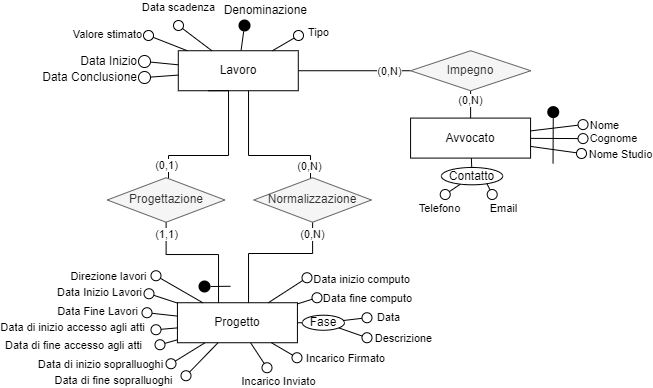
\includegraphics[scale=0.6]{../Img/DBSchemes/Accorpamento-Lavoro.png}
				\end{figure}
		\newpage	
		\subsubsection{Generalizzazione Cliente}
			Cliente è una generalizzazione totale che presenta 3 figlie: Condominio, Persona e Impresa. Analizziamo l'effetto delle diverse tecniche.
		
			\paragraph{Accorpamento delle figlie in Cliente}
				Applicando questa tecnica trasferiremmo gli attributi delle figlie all'interno dell'entità Cliente, dovendo conseguentemente aggiungere un attributo per poter specificare il tipo, portando inoltre alla presenza di attributi con valore nullo a seconda di quest'ultimo: quest'ultima considerazione risulta essere una criticità a causa dell'entità Persona che presenta un notevole numero di attributi non comuni con le altre entità figlie; accorpare Persona in Cliente a causa del rilevante spreco di memoria non risulta essere la scelta migliore. Per quanto riguarda le altre due entità figlie invece, applicare questa tecnica risulta essere un'ottima idea, poiché possiedono uno e zero attributi unici. C'è da considerare però che quest'ultime due entità figlie presentano entrambe una relazione con Persona, pertanto in caso di accorpamento si dovrà procedere aggiungendo due vincoli che impediscano relazioni scorrette. Tutte e 3 le figlie presentano le stesse operazioni, non sono presenti infatti operazioni uniche per un figlio, ad eccezione per quelle che riguardano le due relazioni particolari.
			
			\paragraph{Accorpamento di Cliente nelle figlie}
				Questa tecnica prevede che l'entità Cliente e i suoi attributi collassino sulle figlie, e risulta applicabile solo nei casi di generalizzazione totale, come questo. Con questa tecnica si eviterebbero gli sprechi di attributi dovuti ad attributi nulli che si avrebbero con la prima tecnica, ed inoltre rispetto alla terza tecnica, che analizzeremo successivamente, si evita di dover accedere all'entità padre per accedere alle figlie, diminuendo quindi gli accessi; come per la generalizzazione Lavoro anche in questo questa tecnica non risulta essere particolarmente vantaggiosa, poiché la maggior parte delle operazioni che riguardano un cliente si fermano all'entità padre. Applicare questa tecnica non presenta però neanche particolari svantaggi, le relazioni passerebbero dall'essere 3 all'essere 9, il che non risulta essere limitante.
			
			\paragraph{Sostituzione della generalizzazione con associazioni}
				Poiché la maggior parte delle operazioni riguardanti i Clienti non arrivano alle figlie, l'aumento di accessi dovuti a l'applicazione di questa tecnica risulta essere poco rilevante. C'è inoltre da osservare che questa tecnica permetterebbe di avere entità con un numero di attributi più basso, e data la presenza dell'entità Persona, il cui accorpamento sull'entità padre risulta svantaggioso, si può considerare di utilizzare questa tecnica in combinazione con le altre.
			
			\paragraph{Decisione}
			Anche in questo caso in seguito all'analisi abbiamo deciso di proseguire con una tecnica mista: abbiamo deciso di accorpare nell'entità Cliente le entità Condominio ed Impresa, utilizzando quindi la prima tecnica, e di aggiungere una relazione tra Cliente e Persona, utilizzando perciò la terza tecnica. Così facendo si hanno al massimo 2 attributi nulli a causa dell'accorpamento, e si effettuerà un accesso in più solo in caso servano dati specifici dell'entità Persona.
			Analizziamo le conseguenza:
			\begin{itemize}
				\item L'entità Cliente presenta ora l'attributo \textbf{Tipo} per poter descrivere di che tipologia di cliente si tratta.
				\item L'entità Cliente presenta ora l'attributo \textbf{Denominazione}. L'aggiunta di questo attributo porta all'aggiunta di \textbf{un vincolo}: Denominazione può assumere valori non nulli solo per clienti di tipo "Condominio" e di tipo "Impresa". Normalmente il vincolo avrebbe dovuto permetterlo solo alle Imprese, ma durante questa fase abbiamo realizzato che anche i condomini possono presentare una Denominazione, e abbiamo deciso quindi di comprenderli.
				\item L'entità Cliente presenta ora le relazioni \textbf{Amministrazione} e \textbf{Rappresentanza} con Persona, è pertanto necessario aggiungere \textbf{quattro vincoli}: il primo impone che la relazione Amministrazione sia presente solo nel caso l'attributo Tipo assuma il valore "Condominio"; il secondo vincolo fa lo stesso ma con la relazione Rappresentazione e nel caso Tipo assuma il valore "Impresa"; il terzo vincolo impone che i clienti con Tipo "Condominio" abbiano almeno una relazione Amministrazione con Persona; il quarto vincolo fa lo stesso ma con i clienti di tipo "Impresa" e la relazione Rappresentanza.
				\item L'entità Cliente presenta ora la relazione \textbf{Personificazione} con Persona
			\end{itemize}
			\begin{figure}[H]
				\centering
				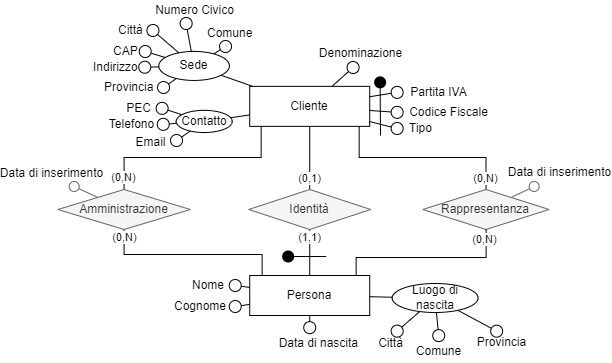
\includegraphics[scale=0.5]{../Img/DBSchemes/Accorpamento-Cliente.png}
			\end{figure}
		\newpage
			
			
	
	\subsection{Partizionamento/Accorpamento di Concetti}
	\subsubsection{Partizionamenti di concetti}
		Analizzando lo schema abbiamo trovato due attributi multivalore che portano ad un partizionamento di concetti.
		\paragraph{CONTATTO}
		Il primo attributo multivalore trovato è Contatto, un attributo ricorrente che raggruppa Telefono, Email e PEC. Poiché Clienti, Collaboratori, Tecnici e Avvocati posso avere molteplici contatti, abbiamo deciso di creare una nuova entità \textbf{Contatto} con due attributi:
		\begin{itemize} 
			\item\textbf{Tipo}: indica di che tipo di contatto si tratta;
			\item \textbf{Dato}: indica il valore del contatto in considerazione.
		\end{itemize} 	
		In seguito al partizionamento la relazione tra le entità coinvolte è la seguente:
		\begin{figure}[H]
			\centering
			\includegraphics[scale=0.4]{../Img/DBSchemes/Contatto.png}
		\end{figure}
		E' necessario aggiungere \textbf{un vincolo} che imponga che Contatto presenti solo una relazione tra quelle presenti.
		
		\paragraph{FASE}
		Il secondo attributo multivalore trovato è Fase, presente nell'entità Progetto per aggiungere informazioni riguardanti la situazione in cui si trova il progetto in una determinata data. Si è quindi deciso di aggiungere l'entità Fase con due attributi:
		\begin{itemize}
			\item \textbf{Descrizione}: descrive la situazione in cui si trova il progetto nella data specificata;
			\item \textbf{Data}: la data a cui fa riferimento la descrizione.
		\end{itemize}
		In seguito al partizionamento la relazione tra le entità coinvolte è la seguente:
		\begin{figure}[H]
			\centering
			\includegraphics[scale=0.5]{../Img/DBSchemes/Fase.png}
		\end{figure}
	
	\subsubsection{Accorpamenti di concetti}
		Analizzando lo schema abbiamo deciso di effettuare un accorpamento, ovvero unificare le relazioni Amministrazione e Rappresentanza in un'unica relazione Rappresentanza. Questo accorpamento avviene poiché i due concetti sono estremamente simili, trattandosi in entrambi i casi del rappresentante di un certo cliente. Poiché solo i clienti di Tipo "Impresa" potevano presentare la relazione Amministrazione, e solo i clienti di Tipo "Condominio" potevano presentare la relazione "Rappresentanza", è chiaro che a distinguere se si tratti di una relazione o dell'altra è l'attributo tipo presente sull'entità Cliente, ma poiché non esistono operazioni che effettuano accessi alla relazione Rappresentanza senza accedere all'entità Cliente, questo accorpamento non comporta accessi in più.
		Lo schema riguardante le entità coinvolte è il seguente:
		\begin{figure}[H]
			\centering
			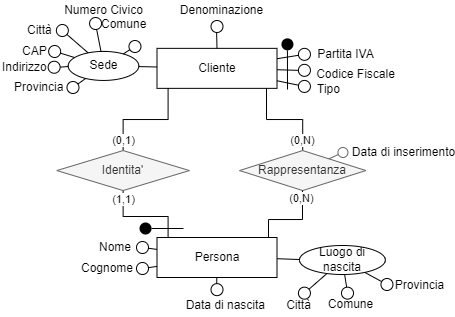
\includegraphics[scale=0.5]{../Img/DBSchemes/Rappresentanza.png}
		\end{figure}
		
	\subsubsection{Elenco degli Identificatori Principali}
	Abbiamo deciso di assegnare a contatto un ID incrementale, poiché non riteniamo non siano presenti attributi che si prestino ad essere identificatori.
	\begin{longtable}{|p{3cm}|p{12cm}|}
		\hline
		\textbf{Entità} & \textbf{Identificatore} \\
		\hline
		Lavoro & Denominazione, Tipo\\
		\hline
		Progetto & Denominazione, Tipo\\
		\hline
		Fase & Denominazione, Data, Descrizione\\
		\hline
		File & Directory\\
		\hline
		Tecnico & Codice Fiscale\\
		\hline 
		Attestato & No. identificativo, Tipo\\
		\hline
		Avvocato & Nome, Cognome, Studio\\
		\hline
		Collaboratore & Partita IVA, Codice Fiscale \\
		\hline
		Struttura & CAP, Indrizzo, Numero Civico\\
		\hline
		Cliente & Partita IVA, Codice Fiscale, Tipo\\
		\hline
		Persona & Partita IVA, Codice Fiscale, Tipo\\
		\hline
		Contatto & ID\\
		\hline
	\end{longtable}
	\newpage
	\subsection{Schema Ristrutturato}
		\begin{figure}[H]
			\centering
			\makebox[\textwidth]{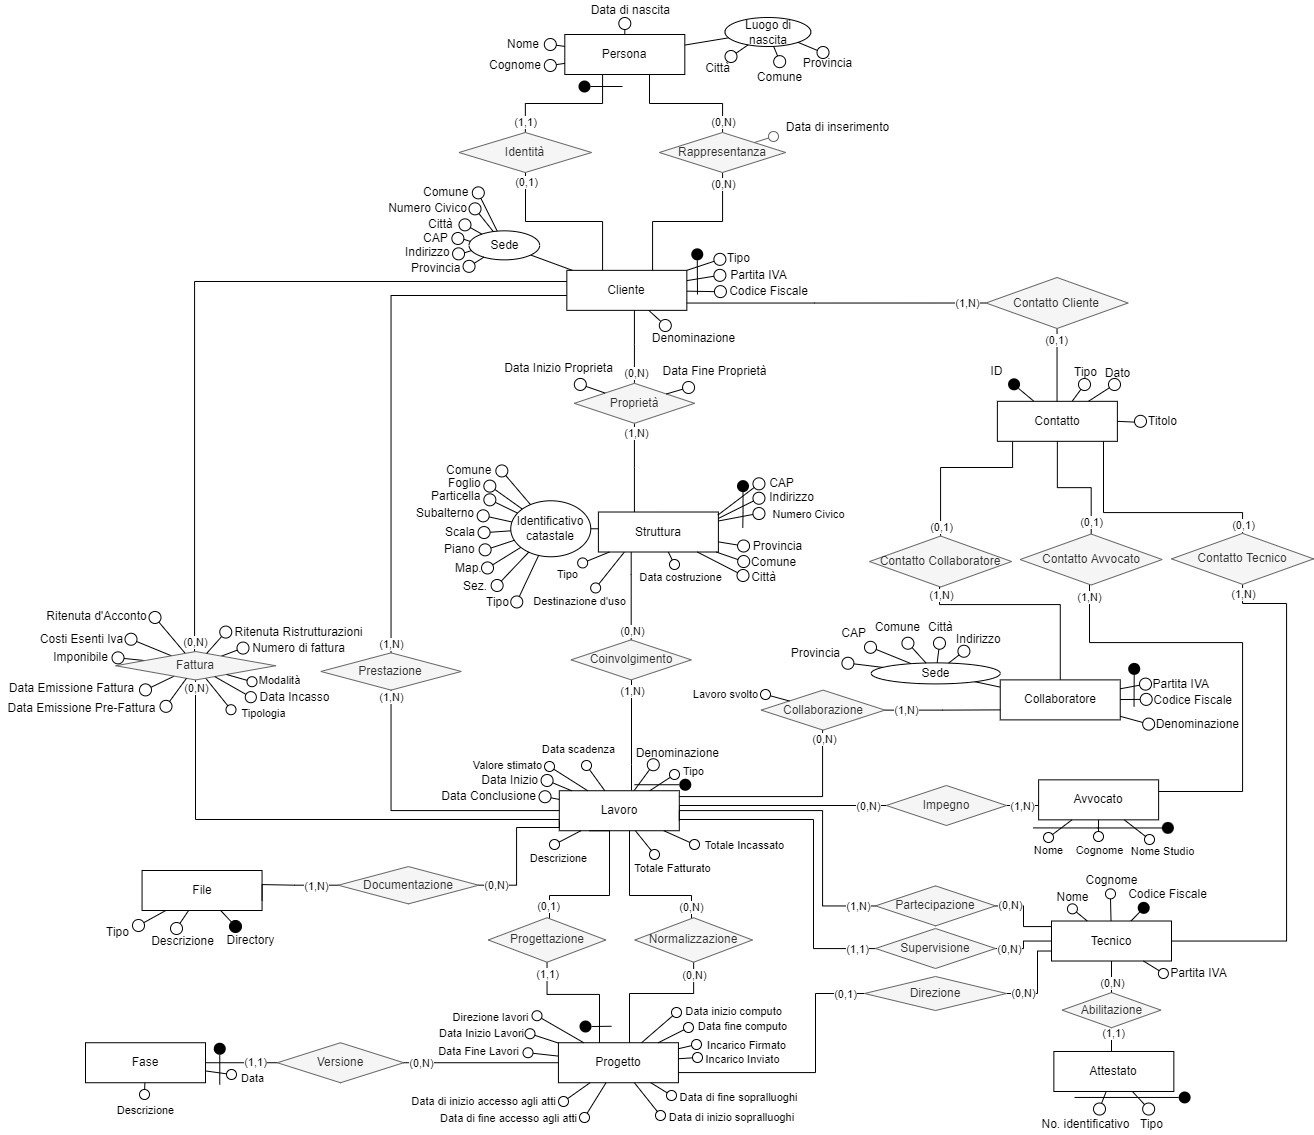
\includegraphics[scale=0.43]{../Img/DBSchemes/Ristrutturato.png}}
                        \caption{Schema Ristrutturato}
		\end{figure}
	\newpage
	\section{Normalizzazione}
	\subsection{Associazioni}
	Nel diagramma logico sono presenti solamente relazioni binarie, pertanto per definizione risultano essere in forma normale di Boyce e Codd
	\subsection{Entità}
        \begin{longtable}{|p{8cm}|r|}
        \hline
            Attestato & Non vi sono dipendenze funzionali non banali \\
	\hline
            Avvocato & Non vi sono dipendenze funzionali non banali \\
	\hline
            Cliente & Non vi sono dipendenze funzionali non banali \\
	\hline
            Collaboratore & Non vi sono dipendenze funzionali non banali \\
	\hline
            Contatto & Non vi sono dipendenze funzionali non banali \\
	\hline
            Fase & Non vi sono dipendenze funzionali non banali \\
	\hline
            File & Non vi sono dipendenze funzionali non banali \\
	\hline
            Lavoro & Non vi sono dipendenze funzionali non banali \\
	\hline
            Persona & Non vi sono dipendenze funzionali non banali \\
	\hline
            Persone & Non vi sono dipendenze funzionali non banali \\
	\hline
            Progetto & Non vi sono dipendenze funzionali non banali \\
	\hline
            Struttura & Non vi sono dipendenze funzionali non banali \\
	\hline
            Tecnico & Non vi sono dipendenze funzionali non banali \\
	\hline    
        \end{longtable} 
	\newpage
	\section{Traduzione verso il Modello Logico}
	\begin{longtable}{|p{3cm}|p{12cm}|}
		\hline
		\textbf{Relationship} & \textbf{Traduzione} \\
		\hline
		Lavoro & Lavoro(\underline{Denominazione}, \underline{Tipo}, Descrizione, Data Inizio, Data Conclusione, Supervisore,  TotFat, TotInc, ValoreStim, Scadenza) \\
		\hline
		Progetto & Progetto(\underline{Denominazione}, \underline{Tipo}, InizioAccessi, FineAccessi, InizioSopralluoghi, FineSopralluoghi, InizioComputo, FineComputo, IncFirmato, IncInviato, DirLavori, Direttore, InizioLavori, FineLavori)\\
		\hline
		Normalizzazione & Normaliz(\underline{DenomCertificato}, \underline{TipoCertificato}, \underline{DenomProg}, \underline{TipoProg}) \\
		\hline
		Fase & Fase(\underline{Denominazione}, \underline{Tipo}, \underline{Data}, Descrizione)\\
		\hline
		File & File(\underline{Directory}, Descrizione, Tipo) \\
		\hline
		Documentazione & Documentaz(\underline{FileDir}, \underline{DenomLavoro}, \underline{TipoLavoro})\\
		\hline
		Tecnico & Tecnico(\underline{CF}, Nome, Cognome, PartitaIVA)\\
		\hline 
		Partecipazione & Partecip(\underline{DenomLavoro}, \underline{Tipo}, \underline{CF}) \\
		\hline
		Attestato & Attestato(\underline{ID}, \underline{Tipo}, Tecnico) \\
		\hline
		Avvocato & Avvocato(\underline{Nome}, \underline{Cognome}, \underline{Studio})\\
		\hline
		Impegno & Impegno(\underline{Denominazione}, \underline{Tipo}, \underline{Nome}, \underline{Cognome}, \underline{Studio})\\
		\hline
		Collaboratore & Collaboratore(\underline{PartitaIVA}, \underline{CF}, Denominazione, Provincia, CAP, Comune, Citta, Indirizzo)\\
		\hline
		Collaborazione & Collaborazione(\underline{Denominazione}, \underline{Tipo}, \underline{PartitaIVA}, \underline{CF})\\
		\hline
		Struttura & Struttura(\underline{CAP}, \underline{Indrizzo}, \underline{NumCiv}, Provincia, Comune, Citta, DataCostruzione, ComuneCatastale, Foglio, Particella, Subalterno, Scala, Piano, Map, Sezione, Tipo)\\
		\hline
		Coinvolgimento & Coinvolgimento(\underline{Denominazione}, \underline{Tipo}, \underline{CAP}, \underline{Indrizzo}, \underline{NumeroCiv})\\
		\hline
		Cliente & Cliente(\underline{PartitaIVA}, \underline{CF}, \underline{Tipo}, Denominazione, Comune, NumCiv, Citta, CAP, Indirizzo, Provincia)\\
		\hline
		Persona & Persona(\underline{PartitaIVA}, \underline{CF}, \underline{Tipo}, Nome, Cognome, DataNascita, Citta, Comune, Provincia)\\
		\hline
		Rappresentanza & Rappresentanza(\underline{PartitaIvaCliente}, \underline{CFCliente}, \underline{PartitaIvaPersona}, \underline{CFPersona}, DataInserimento)\\
		\hline
		Proprieta & Proprieta(\underline{PartitaIVA}, \underline{CF}, \underline{CAP}, \underline{Indrizzo}, \underline{NumCiv}, DataInizioProp, DataFineProp)\\
		\hline
		Prestazione &Prestazione(\underline{Denominazione}, \underline{Tipo}, \underline{PartitaIVA}, \underline{CF})\\ 
		\hline
		Fattura & Fattura(\underline{NumeroFat}, \underline{DenomLavoro}, \underline{TipoLavoro}, \underline{PartitaIVA}, \underline{CF}, Tipologia, Modalita, Imponibile, CostiEsentiIVA, RitenutaAcc, RitenutaRist, DataEmissioneFat, DataEmissionePreFat, DataIncasso)\\
		\hline
		Contatto & Contatto(\underline{ID}, Titolo, PartitaIVACliente, CFCliente, TipoCliente, PartitaIVACollab, CFCollab, NomeAvv, CognomeAvv, StudioAvv, CFTecnico, Tipo, Dato)\\
		\hline
	\end{longtable}
	
		\begin{longtable}{|p{9cm}|p{8cm}|}
		\hline
		\textbf{Traduzione} & \textbf{Vincoli di riferimenti} \\
		\hline
		Lavoro(\underline{Denominazione}, \underline{Tipo}, Descrizione, Data Inizio, Data Conclusione, \hl{Supervisore},  TotFat, TotInc, ValoreStim, Scadenza) & Supervisore  -> Tecnico.CF \\
		\hline
		Progetto(\underline{\hl{Denominazione}}, \underline{\hl{Tipo}}, InizioAccessi, FineAccessi, InizioSopralluoghi, FineSopralluoghi, InizioComputo, FineComputo, IncFirmato, IncInviato, DirLavori, \hl{Direttore}, InizioLavori, FineLavori) & Denominazione -> Lavoro.Denominazione \newline Tipo -> Lavoro.Tipo \newline Direttore -> Tecnico.CF\\
		\hline
		Normaliz(\underline{\hl{DenomCertificato}}, \underline{\hl{DenomProg}}) & DenomCertificato -> Lavoro.Denominazione \newline Progetto.Denominazione \\
		\hline
		Fase(\underline{\hl{DenomLavoro}}, \underline{Data}, Descrizione) & DenomLavoro -> Lavoro.Denominazione\\
		\hline
		File(\underline{Directory}, Descrizione, Tipo) & ***\\
		\hline
		Documentaz(\underline{\hl{FileDir}}, \underline{\hl{DenomLavoro}}, \underline{\hl{TipoLavoro}}) & FileDir -> File.Directory \newline DenomLavoro -> Lavoro.Denominazione \newline TipoLavoro -> Lavoro.Tipo\\
		\hline
		Tecnico(\underline{CF}, Nome, Cognome, PartitaIVA) & ***\\
		\hline 
		Partecip(\underline{\hl{DenomLavoro}}, \underline{\hl{Tipo}}, \underline{\hl{CF}}) & DenomLavoro -> Lavoro.Denominazione \newline Tipo Lavoro.Tipo \newline CF -> Tecnico.CF\\
		\hline
		Attestato(\underline{ID}, \underline{Tipo}, \hl{Tecnico}) & Tecnico -> Tecnico.CF\\
		\hline
		Avvocato(\underline{Nome}, \underline{Cognome}, \underline{Studio}) & ***\\
		\hline
		Impegno(\underline{\hl{Denominazione}}, \underline{\hl{Tipo}}, \underline{\hl{Nome}}, \underline{\hl{Cognome}}, \underline{\hl{Studio}}) & Denominazione -> Lavoro.Denominazione \newline Tipo -> Lavoro.Tipo \newline Nome -> Avvocato.Nome \newline Cognome -> Avvocato.Cognome \newline Studio -> Avvocato.Studio\\
		\hline
		Collaboratore(\underline{PartitaIVA}, \underline{CF}, Denominazione, Provincia, CAP, Comune, Citta, Indirizzo) & ***\\
		\hline
		Collaborazione(\underline{\hl{Denominazione}}, \underline{\hl{Tipo}}, \underline{\hl{PartitaIVA}}, \underline{\hl{CF}}) & Denominazione -> Lavoro.Denominazione \newline Tipo -> Lavoro.Denominazione \newline PartitaIVA -> Collaboratore.PartitaIva \newline CF -> Collaboratore.CF\\
		\hline
		Struttura(\underline{CAP}, \underline{Indrizzo}, \underline{NumCiv}, Provincia, Comune, Citta, DataCostruzione, ComuneCatastale, Foglio, Particella, Subalterno, Scala, Piano, Map, Sezione, Tipo) & ***\\
		\hline
		Coinvolgimento(\underline{\hl{Denominazione}}, \underline{\hl{Tipo}}, \underline{\hl{CAP}}, \underline{\hl{Indrizzo}}, \underline{\hl{NumeroCiv}}) & Denominazione -> Lavoro.Denominazione\newline Tipo -> Lavoro.Tipo \newline CAP -> Struttura.CAP \newline Indirizzo -> Struttura.Indirizzo \newline NumeroCiv ->  Struttura.NumeroCiv\\
		\hline
		Cliente(\underline{PartitaIVA}, \underline{CF}, Tipo, Denominazione, Comune, NumCiv, Citta, CAP, Indirizzo, Provincia) & ***\\
		\hline
		Persona(\underline{\hl{PartitaIVA}}, \underline{\hl{CF}}, Nome, Cognome, DataNascita, Citta, Comune, Provincia) & PartitaIVA -> Cliente.PartitaIVA \newline CF -> Cliente.CF \\
		\hline
		Rappresentanza(\underline{\hl{PartitaIvaCliente}}, \underline{\hl{CFCliente}}, \underline{\hl{PartitaIvaPersona}}, \underline{\hl{CFPersona}}, DataInserimento) & PartitaIVACliente -> Cliente.PartitaIva \newline CFCliente Cliente.CF \newline PartitaIvaPersona -> Persona.PartitaIVA\newline CFPersona -> Persona.CF \\
		\hline
		Proprieta(\underline{\hl{PartitaIVA}}, \underline{\hl{CF}}, \underline{\hl{CAP}}, \underline{\hl{Indrizzo}}, \underline{\hl{NumCiv}}, DataInizioProp, DataFineProp) & PartitaIVA -> Cliente.PartitaIva\newline CF -> Cliente.CF \newline CAP ->Struttura.CAP \newline Indrizzo -> Struttura.Indrizzo \newline NumCiv -> Struttura.NumCiv\\
		\hline
		Prestazione(\underline{\hl{Denominazione}}, \underline{\hl{Tipo}}, \underline{\hl{PartitaIVA}}, \underline{\hl{CF}}) & Denominazione -> Lavoro.Denominazione \newline Tipo -> Lavoro.Tipo \newline PartitaIVA -> Cliente.PartitaIVA \newline CF -> Cliente.CF\\ 
		\hline
		Fattura(\underline{NumeroFat}, \underline{\hl{DenomLavoro}}, \underline{\hl{TipoLavoro}}, \underline{\hl{PartitaIVA}}, \underline{\hl{CF}}, Tipologia, Modalita, Imponibile, CostiEsentiIVA, RitenutaAcc, RitenutaRist, DataEmissioneFat, DataEmissionePreFat, DataIncasso) & DenomLavoro -> Lavoro.Denominazione \newline Tipo -> Lavoro.Tipo \newline PartitaIVA -> Cliente.PartitaIVA \newline CF -> Cliente.CF\\
		\hline
		Contatto(\underline{Titolo}, \underline{\hl{PartitaIVACliente}}, \underline{\hl{CFCliente}}, \underline{\hl{PartitaIVACollab}}, \underline{\hl{CFCollab}}, \underline{\hl{NomeAvv}}, \underline{\hl{CognomeAvv}}, \underline{\hl{StudioAvv}}, \underline{\hl{CFTecnico}}, Tipo, Dato) & PartitaIVACliente -> Cliente.PartitaIVA  \newline CFCliente -> Cliente.CF\newline PartitaIVACollab Collavoratore.PartitaIVA\newline CFCollab Collaboratore.CF \newline NomeAvv -> Avvocato.Nome\newline CognomeAvv -> Avvocato.Cognome\newline StudioAvv Avvocato.Studio \newline CFTecnico -> Tecnico.CF\\
		\hline
	\end{longtable}

\chapter{Realizzazione SQL e Testing}
	Riportiamo di seguito la realizzazione della base di dati in linguaggio SQL. Per permettere una migliore comprensione delle query sarà presente uno screenshot del risultato per quelle che riteniamo esse le query piu importanti, evitando di inserire quelle che riteniamo superflue.
	Per riuscire a provare in maniera piu realistica la correttezza delle query, abbiamo deciso di inserire i dati fittizi utilizzando Faker, una libreria di Python che ci ha permesso di inserire un grande quantitativo di dati.
\section{Definizione Relazioni ed inserimento dati}
\subsection{Tecnico}
\begin{verbatim}
	CREATE TABLE Tecnico(
	CF char(16) NOT NULL PRIMARY KEY,
	Nome varchar(30) NOT NULL,
	Cognome varchar(30) NOT NULL,
	PartitaIVA char(11) DEFAULT NULL
	)Engine=InnoDB;
\end{verbatim}
\begin{figure}[H]
	\centering
	\makebox[\textwidth]{\includegraphics[scale=0.43]{../Img/Queries/Tecnico.png}}
	\caption{Schema Ristrutturato}
\end{figure}
\subsection{Lavoro}
\begin{verbatim}
	CREATE TABLE Lavoro(
	Denominazione varchar(50) NOT NULL,
	Tipo varchar(25) NOT NULL,
	Descrizione varchar(5000) DEFAULT NULL,
	DataInizio date NOT NULL, 
	DataConclusione date DEFAULT NULL,
	Supervisore char(16) NOT NULL,
	TotFat decimal(10,2) DEFAULT NULL,
	TotInc decimal(10,2) DEFAULT NULL,
	ValoreStim decimal(10,2) DEFAULT NULL, 
	Scadenza date DEFAULT NULL, 
	PRIMARY KEY (Denominazione, Tipo),
	FOREIGN KEY (Supervisore) REFERENCES Tecnico(CF),
	constraint checkDataConcl 
		CHECK( DataConclusione > DataInizio OR 
			DataConclusione IS NULL),
	constraint checkVal 
		CHECK((ValoreStim IS NOT NULL AND Tipo LIKE "PER%") OR (ValoreStim IS NULL))
	)Engine=InnoDB;
\end{verbatim}
\begin{figure}[H]
	\centering
	\makebox[\textwidth]{\includegraphics[scale=0.43]{../Img/Queries/Lavoro.png}}
	\caption{Schema Ristrutturato}
\end{figure}
\subsection{Progetto}
\begin{verbatim}
	CREATE TABLE Progetto(
	PRDenominazione varchar(50) NOT NULL,
	PRTipo varchar(25) NOT NULL
	check (PRTipo LIKE "PRO%"), 
	InizioAccessi date DEFAULT NULL,
	FineAccessi date DEFAULT NULL,
	InizioSopralluoghi date DEFAULT NULL,
	FineSopralluoghi date DEFAULT NULL,
	InizioComputo date DEFAULT NULL,
	FineComputo date DEFAULT NULL,
	IncFirmato boolean DEFAULT FALSE,
	IncInviato boolean DEFAULT FALSE,
	DirLavori  boolean DEFAULT FALSE,
	Direttore char(16) NULL,
	InizioLavori date DEFAULT NULL,
	FineLavori date DEFAULT NULL,
	
	PRIMARY KEY (PRDenominazione, PRTipo),
	FOREIGN KEY (PRDenominazione, PRTipo) REFERENCES Lavoro(Denominazione,Tipo),
	constraint checkFineAccessi 
	check (FineAccessi IS NULL 
		OR (FineAccessi IS NOT NULL AND FineAccessi > InizioAccessi)),
	constraint checkFineSopr 
	check (FineSopralluoghi IS NULL 
		OR (FineSopralluoghi IS NOT NULL AND FineSopralluoghi > InizioSopralluoghi)),
	constraint checkFineComp 
	check (FineComputo IS NULL 
		OR (FineComputo IS NOT NULL AND FineComputo > InizioComputo)),
	constraint checkIncFirm 
	check (IncFirmato IS FALSE 
		OR (IncFirmato IS NOT FALSE AND IncInviato = True)),
	constraint checkDir
	check (Direttore IS NULL 
		OR (Direttore IS NOT NULL AND DirLavori = True)),
	constraint checkFineLav 
	check (FineLavori IS NULL 
		OR (FineLavori IS NOT NULL AND FineLavori > InizioLavori))
	)Engine=InnoDB;
\end{verbatim}
\begin{figure}[H]
	\centering
	\makebox[\textwidth]{\includegraphics[scale=0.43]{../Img/Queries/Progetto.png}}
	\caption{Schema Ristrutturato}
\end{figure}
\subsection{Normaliz}
\begin{verbatim}
	CREATE TABLE Normaliz(
	DenomCertificato varchar(50) NOT NULL,
	TipoCertificato varchar(25) NOT NULL check(TipoCertificato LIKE "CER%"),
	DenomProgetto varchar(50) NOT NULL,
	TipoProgetto varchar(25) NOT NULL  check(TipoProgetto LIKE "PROV%"),
	PRIMARY KEY (DenomProgetto, DenomCertificato),
	FOREIGN KEY (DenomCertificato, TipoCertificato) REFERENCES Lavoro(Denominazione, Tipo),
	FOREIGN KEY (DenomProgetto, TipoProgetto) REFERENCES Lavoro(Denominazione, Tipo),
	CONSTRAINT checkTipiNorm 
	CHECK (TipoCertificato LIKE 'CER%' AND TipoProgetto LIKE 'PRO%')
	)Engine=InnoDB;
\end{verbatim}
\begin{figure}[H]
	\centering
	\makebox[\textwidth]{\includegraphics[scale=0.43]{../Img/Queries/Normaliz.png}}
	\caption{Schema Ristrutturato}
\end{figure}
\subsection{Fase}
\begin{verbatim}
	CREATE TABLE Fase(
	Denominazione varchar(50) NOT NULL,
	Tipo varchar(25) NOT NULL,
	DataFase date NOT NULL,
	Descrizione varchar(200) NOT NULL,
	
	PRIMARY KEY (Denominazione, Tipo, DataFase),
	FOREIGN KEY (Denominazione, Tipo) REFERENCES Lavoro(Denominazione, Tipo),
	CONSTRAINT checkTipoFase CHECK (Tipo LIKE 'PRO%')
	)Engine=InnoDB;
\end{verbatim}
\begin{figure}[H]
	\centering
	\makebox[\textwidth]{\includegraphics[scale=0.43]{../Img/Queries/Fase.png}}
	\caption{Schema Ristrutturato}
\end{figure}
\subsection{FileLavoro}
\begin{verbatim}
	CREATE TABLE FileLavoro(
	Directory varchar(100) PRIMARY KEY,
	Descrizione varchar(500),
	Tipo varchar(10) COMMENT 'estensione del file'
	)Engine=InnoDB;
\end{verbatim}
\begin{figure}[H]
	\centering
	\makebox[\textwidth]{\includegraphics[scale=0.43]{../Img/Queries/FileLavoro.png}}
	\caption{Schema Ristrutturato}
\end{figure}
\subsection{Documentazione}
\begin{verbatim}
	CREATE TABLE Documentaz(
	FileDir varchar(100) NOT NULL,
	DenomLavoro varchar(50) NOT NULL,
	TipoLavoro varchar(25) NOT NULL,
	PRIMARY KEY (FileDir, DenomLavoro, TipoLavoro),
	FOREIGN KEY (FileDir)    			  REFERENCES FileLavoro(Directory),
	FOREIGN KEY (DenomLavoro, TipoLavoro) REFERENCES Lavoro(Denominazione, Tipo)
	)Engine=InnoDB;
\end{verbatim}
\begin{figure}[H]
	\centering
	\makebox[\textwidth]{\includegraphics[scale=0.43]{../Img/Queries/Documentaz.png}}
	\caption{Schema Ristrutturato}
\end{figure}
\subsection{Partecip}
\begin{verbatim}
	CREATE TABLE Partecip(
	DenomLavoro varchar(50) NOT NULL,
	PTipo varchar(25) NOT NULL,
	PTecnico char(16) NOT NULL,
	PRIMARY KEY (DenomLavoro, PTipo, PTecnico),
	FOREIGN KEY (DenomLavoro, PTipo) REFERENCES Lavoro(Denominazione, Tipo),
	FOREIGN KEY (PTecnico) REFERENCES Tecnico(CF)
	)Engine=InnoDB;
	
\end{verbatim}
\begin{figure}[H]
	\centering
	\makebox[\textwidth]{\includegraphics[scale=0.43]{../Img/Queries/Partecip.png}}
	\caption{Schema Ristrutturato}
\end{figure}
\subsection{Attestato}
\begin{verbatim}
	CREATE TABLE Attestato(
	ID varchar(100) NOT NULL,
	Tipo varchar (10) NOT NULL,
	Tecnico char(16) NOT NULL,
	PRIMARY KEY (ID,Tipo),
	FOREIGN KEY (Tecnico) REFERENCES Tecnico(CF)
	)Engine=InnoDB;
\end{verbatim}
\begin{figure}[H]
	\centering
	\makebox[\textwidth]{\includegraphics[scale=0.43]{../Img/Queries/Attestato.png}}
	\caption{Schema Ristrutturato}
\end{figure}
\subsection{Avvocato}
\begin{verbatim}
	CREATE TABLE Avvocato(
	Nome varchar(30) NOT NULL,
	Cognome varchar(30) NOT NULL,
	Studio varchar(80) DEFAULT NULL,
	PRIMARY KEY(Nome, Cognome, Studio)
	)Engine=InnoDB;
\end{verbatim}
\begin{figure}[H]
	\centering
	\makebox[\textwidth]{\includegraphics[scale=0.43]{../Img/Queries/Avvocato.png}}
	\caption{Schema Ristrutturato}
\end{figure}
\subsection{Collaboratore}
\begin{verbatim}
	CREATE TABLE Collaboratore(
	PartitaIVA char(11) NOT NULL,
	CF char(16) NOT NULL,
	Denominazione varchar(100),
	Provincia varchar(50) NOT NULL,
	CAP varchar(5) NOT NULL,
	Comune varchar(50) NOT NULL,
	Citta varchar(50) NOT NULL,
	Indirizzo varchar(70) NOT NULL,
	
	PRIMARY KEY(PartitaIVA, CF)
	)Engine=InnoDB;
\end{verbatim}
\begin{figure}[H]
	\centering
	\makebox[\textwidth]{\includegraphics[scale=0.43]{../Img/Queries/Collaboratore.png}}
	\caption{Schema Ristrutturato}
\end{figure}
\subsection{Struttura}
\begin{verbatim}
	CREATE TABLE Struttura(
	CAP char(5) NOT NULL,
	Indirizzo varchar(70) NOT NULL,
	NumCiv varchar(6) NOT NULL,
	Provincia varchar(30) NOT NULL,
	Citta varchar(30) NOT NULL,
	Comune varchar(50) NOT NULL,
	DataCostruzione date DEFAULT NULL,
	ComuneCatastale varchar(50) DEFAULT NULL,
	Foglio INT DEFAULT NULL CHECK (Foglio=NULL OR Foglio>=0),
	Particella INT DEFAULT NULL CHECK (Particella=NULL OR Particella>=0),
	Subalterno INT DEFAULT NULL CHECK (Subalterno=NULL OR Subalterno>=0),
	Scala INT DEFAULT NULL CHECK (Scala=NULL OR Scala>=0),
	Piano INT DEFAULT NULL CHECK (Piano=NULL OR Piano>=0),
	Sezione INT DEFAULT NULL CHECK (Sezione=NULL OR Sezione>=0),
	Tipo varchar(50) DEFAULT NULL,
	
	PRIMARY KEY(CAP, Indirizzo, NumCiv)
	)Engine=InnoDB;
\end{verbatim}
\begin{figure}[H]
	\centering
	\makebox[\textwidth]{\includegraphics[scale=0.43]{../Img/Queries/Struttura.png}}
	\caption{Schema Ristrutturato}
\end{figure}
\subsection{Coinvolgim}
\begin{verbatim}
	CREATE TABLE Coinvolgim(
	Denominazione varchar(50) NOT NULL,
	Tipo varchar(25) NOT NULL,
	CAP varchar(5) NOT NULL,
	Indirizzo varchar(70) NOT NULL, 
	NumCiv varchar(6) NOT NULL,
	
	PRIMARY KEY(Denominazione, Tipo, CAP, Indirizzo, NumCiv),
	FOREIGN KEY (Denominazione, Tipo) REFERENCES Lavoro(Denominazione, Tipo),
	FOREIGN KEY (CAP, Indirizzo, NumCiv) REFERENCES Struttura(CAP, Indirizzo, NumCiv)
	)Engine=InnoDB;
\end{verbatim}
\begin{figure}[H]
	\centering
	\makebox[\textwidth]{\includegraphics[scale=0.43]{../Img/Queries/Coinvolgim.png}}
	\caption{Schema Ristrutturato}
\end{figure}
\subsection{Cliente}
\begin{verbatim}
	/*
	Di seguito troviamo una lista dei valore che puo assumere il valore Tipo:
	---PER Persona
	---IMP Impresa
	---CON Condominio
	*/
	CREATE TABLE Cliente(
	PartitaIVA char(11) NOT NULL,
	CF char(16) NOT NULL,
	Tipo char(3) NOT NULL,
	Denominazione varchar(100) DEFAULT NULL,
	Comune varchar(50) NOT NULL,
	NumeroCiv varchar(6) NOT NULL,
	Citta varchar(30) NOT NULL, 
	CAP char(5) NOT NULL,
	Indirizzo varchar(70) NOT NULL,
	Provincia varchar(30) NOT NULL,
	
	PRIMARY KEY(PartitaIVA, CF),
	Constraint checkTipo CHECK(Tipo='PER' OR Tipo='IMP' OR Tipo='CON')
	)Engine=InnoDB;
\end{verbatim}
\begin{figure}[H]
	\centering
	\makebox[\textwidth]{\includegraphics[scale=0.43]{../Img/Queries/Cliente.png}}
	\caption{Schema Ristrutturato}
\end{figure}
\subsection{Persona}
\begin{verbatim}
	CREATE TABLE Persona(
	PartitaIVA char(11) NOT NULL,
	CF char(16) NOT NULL,
	Nome varchar(30) NOT NULL,
	Cognome varchar(30) NOT NULL,
	DataNascita date DEFAULT NULL,
	Citta varchar(30) DEFAULT NULL,
	Comune varchar(50) DEFAULT NULL,
	Provincia varchar(30) DEFAULT NULL,
	
	PRIMARY KEY(PartitaIVA, CF),
	FOREIGN KEY (PartitaIVA, CF) REFERENCES Cliente(PartitaIVA, CF)
	)Engine=InnoDB;
\end{verbatim}
\begin{figure}[H]
	\centering
	\makebox[\textwidth]{\includegraphics[scale=0.43]{../Img/Queries/Persona.png}}
	\caption{Schema Ristrutturato}
\end{figure}
\subsection{Rappresent}
\begin{verbatim}
	CREATE TABLE Rappresent(
	PartitaIVACliente varchar(11) NOT NULL,
	CFCliente varchar(16) NOT NULL,
	PartitaIVAPersona varchar(11) NOT NULL,
	CFPersona varchar(16) NOT NULL,
	DataInserimento date NOT NULL,
	
	PRIMARY KEY(PartitaIVACliente, CFCliente, PartitaIVAPersona, CFPersona),
	FOREIGN KEY (PartitaIVACliente, CFCliente) REFERENCES Cliente(PartitaIVA, CF),
	FOREIGN KEY (PartitaIVAPersona, CFPersona) REFERENCES Cliente(PartitaIVA, CF)
	)Engine=InnoDB;
\end{verbatim}
\begin{figure}[H]
	\centering
	\makebox[\textwidth]{\includegraphics[scale=0.43]{../Img/Queries/Raprresent.png}}
	\caption{Schema Ristrutturato}
\end{figure}
\subsection{Proprieta}
\begin{verbatim}
	CREATE TABLE Propietà(
	PartitaIVA char(11) NOT NULL,
	CF char(16) NOT NULL,
	CAP char(5) NOT NULL,
	Indirizzo varchar(70) NOT NULL,
	NumeroCiv varchar(6) NOT NULL,
	DataInizioProp date NOT NULL,
	DataFineProp date DEFAULT NULL,
	
	PRIMARY KEY (PartitaIVA, CF, CAP, Indirizzo, NumeroCiv),
	FOREIGN KEY (PartitaIVA, CF) REFERENCES Cliente(PartitaIVA, CF),
	FOREIGN KEY (CAP, Indirizzo, NumeroCiv) REFERENCES Struttura(CAP, Indrizzo, NumeroCiv),
	CHECK (DataInizioProp < DataFineProp),
	CONSTRAINT CheckDate 
	CHECK ((DataInizioProp IS NULL AND DataFineProp IS NULL) 
		OR (DataInizioProp IS NOT NULL AND DataFineProp IS NOT NULL) 
		OR (DataInizioProp IS NOT NULL AND DataFineProp IS NULL)),
	CONSTRAINT CheckPersonaNascita 
	CHECK (((SELECT Tipo FROM Cliente WHERE Cliente.PartitaIVA=PartitaIVA AND Cliente.CF=CF)!='PER')
		OR(DataInizioProp > 
		(SELECT DataNascita FROM Persona, Cliente WHERE Persona.PartitaIVA = Cliente.PartitaIVA AND Persona.CF=Cliente.CF)))
	)Engine=InnoDB;
\end{verbatim}
\begin{figure}[H]
	\centering
	\makebox[\textwidth]{\includegraphics[scale=0.43]{../Img/Queries/Proprieta.png}}
	\caption{Schema Ristrutturato}
\end{figure}
\subsection{Prestaz}
\begin{verbatim}
	CREATE TABLE Prestaz(
	Denominazione varchar(50) NOT NULL,
	Tipo varchar(25) NOT NULL,
	PartitaIVA char(11) NOT NULL,
	CF char(16) NOT NULL,
	
	PRIMARY KEY(Denominazione, Tipo, PartitaIVA, CF),
	FOREIGN KEY (Denominazione, Tipo) REFERENCES Lavoro(Denominazione, Tipo),
	FOREIGN KEY (PartitaIVA, CF) REFERENCES Cliente(PartitaIVA, CF)
	)Engine=InnoDB;
\end{verbatim}
\begin{figure}[H]
	\centering
	\makebox[\textwidth]{\includegraphics[scale=0.43]{../Img/Queries/Prestaz.png}}
	\caption{Schema Ristrutturato}
\end{figure}
\subsection{Fattura}
\begin{verbatim}
	CREATE TABLE Fattura(
	NumeroFat INT NOT NULL,
	DenomLavoro varchar(50) NOT NULL,
	TipoLavoro varchar(25) NOT NULL,
	PartitaIVA char(11) NOT NULL,
	CF char(16) NOT NULL,
	Tipologia varchar(50) NOT NULL,
	Modalita varchar(30) NOT NULL,
	Imponibile INT NOT NULL CHECK(Imponibile>=0),
	CostiEsentiIVA INT NOT NULL CHECK(CostiEsentiIVA>=0),
	RitenutaAcc INT NOT NULL CHECK(RitenutaAcc>=0),
	RitenutaRistr INT NOT NULL CHECK(RitenutaRistr>=0),
	DataFaT date DEFAULT NULL,
	DataPreFat date DEFAULT NULL,
	DataInc date DEFAULT NULL,
	
	PRIMARY KEY(NumeroFat, DenomLavoro, TipoLavoro, PartitaIVA, CF),
	FOREIGN KEY (DenomLavoro, TipoLavoro) REFERENCES Lavoro(Denominazione,Tipo),
	FOREIGN KEY (PartitaIVA, CF) REFERENCES Cliente(PartitaIVA,CF),
	CONSTRAINT CheckDataPre 
	CHECK((DataPreFat IS NULL OR DataFat IS NULL) OR (DataPreFat<=DataFat)),
	CONSTRAINT CheckDataInc 
	CHECK(DataInc>DataFat)
	)Engine=InnoDB;
\end{verbatim}
\begin{figure}[H]
	\centering
	\makebox[\textwidth]{\includegraphics[scale=0.43]{../Img/Queries/Fattura.png}}
	\caption{Schema Ristrutturato}
\end{figure}
\subsection{Contatto}
\begin{verbatim}
	CREATE TABLE Contatto(
	ID INT NOT NULL AUTO_INCREMENT,
	Titolo varchar(100) NOT NULL,
	PartitaIVACliente varchar(11) DEFAULT NULL,
	CFCliente varchar(16) DEFAULT NULL,
	PartitaIVACollab varchar(11) DEFAULT NULL,
	CFCollab varchar(16) DEFAULT NULL,
	NomeAvv varchar(30) DEFAULT NULL,
	CognmomeAvv varchar(30) DEFAULT NULL,
	StudioAVV varchar(50) DEFAULT NULL,
	CFTecnico varchar(16) DEFAULT NULL,
	Tipo varchar(8) NOT NULL,
	Dato varchar(100) NOT NULL,
	
	PRIMARY KEY(ID),
	FOREIGN KEY (PartitaIVACliente, CFCliente) REFERENCES Cliente(PartitaIVA,CF),
	FOREIGN KEY (PartitaIVACollab, CFCollab) REFERENCES Collaboratore(PartitaIVA,CF),
	FOREIGN KEY (NomeAvv, CognmomeAvv, StudioAVV) REFERENCES Avvocato(Nome,Cognome,Studio),
	FOREIGN KEY (CFTecnico) REFERENCES Tecnico(CF),
	
	CONSTRAINT CheckFK 
	CHECK((PartitaIVACliente IS NOT NULL AND CFCliente IS NOT NULL 
	AND PartitaIVACollab IS NULL AND CFCollab IS NULL AND NomeAvv IS NULL 
	AND CognmomeAvv IS NULL AND StudioAVV IS NULL AND CFTecnico IS NULL)
	OR(PartitaIVACliente IS NULL AND CFCliente IS NULL 
	AND PartitaIVACollab IS NOT NULL AND CFCollab IS NOT NULL AND NomeAvv IS NULL 
	AND CognmomeAvv IS NULL AND StudioAVV IS NULL AND CFTecnico IS NULL)
	OR(PartitaIVACliente IS NULL AND CFCliente IS NULL 
	AND PartitaIVACollab IS NULL AND CFCollab IS NULL AND NomeAvv IS NOT NULL 
	AND CognmomeAvv IS NOT NULL AND CFTecnico IS NULL)
	OR(PartitaIVACliente IS NULL AND CFCliente IS NULL 
	AND PartitaIVACollab IS NULL AND CFCollab IS NULL AND NomeAvv IS NULL 
	AND CognmomeAvv IS NULL AND StudioAVV IS NULL AND CFTecnico IS NOT NULL))
	)Engine=InnoDB;
\end{verbatim}
\begin{figure}[H]
	\centering
	\makebox[\textwidth]{\includegraphics[scale=0.43]{../Img/Queries/Contatto.png}}
	\caption{Schema Ristrutturato}
\end{figure}
\newpage
\section{Implementazione e testing delle operazioni}
\subsection{Query di Consultazione}
\subsubsection{Consultazione Totale Fatturato nell'anno corrente}
\begin{verbatim}
	SELECT SUM((Imponibile*1.26)+CostiEsentiIVA+RitenutaAcc) AS 'Fatturato'
	FROM Fattura
	Where YEAR(DataFat)=YEAR(CURDATE())
\end{verbatim}
\begin{figure}[H]
	\centering
	\makebox[\textwidth]{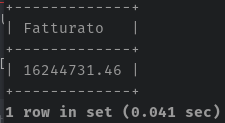
\includegraphics[scale=0.43]{../Img/Queries/1.png}}
\end{figure}
\subsubsection{Consultazione Totale Fatturato coi Lavori iniziati nell'anno corrente}
\begin{verbatim}
	SELECT YEAR(CURDATE()),SUM(TotFat) AS 'Fatturato'
	FROM Lavoro
	Where YEAR(DataInizio)=Year(CURDATE());
\end{verbatim}
	\begin{figure}[H]
	\centering
	\makebox[\textwidth]{\includegraphics[scale=0.43]{../Img/Queries/2.png}}
	\end{figure}
\subsubsection{Consultazione Totale Fatturato diviso per anno}
\begin{verbatim}
	SELECT YEAR(DataFat) AS 'Anno', 
	SUM((Imponibile*1.26)+CostiEsentiIVA+RitenutaAcc) AS 'Totale Fatturato'
	FROM Fattura
	GROUP BY YEAR(DataFat);
\end{verbatim}
\begin{figure}[H]
	\centering
	\makebox[\textwidth]{\includegraphics[scale=0.43]{../Img/Queries/3.png}}
\end{figure}
\subsubsection{Consultazione Collaboratori che hanno lavorato su una determinata Struttura}
	\begin{verbatim}
		SELECT C.Denominazione, C.PartitaIVA, C.CF
		FROM (((Collaboratore AS C 
		INNER JOIN Collaboraz AS CL ON (C.PartitaIVA=CL.PartitaIVA) AND (C.CF=CL.CF))
		INNER JOIN Lavoro AS L ON CL.Denominazione=L.Denominazione AND CL.Tipo=L.Tipo))
		INNER JOIN Coinvolgim AS LS ON (L.Denominazione=LS.Denominazione) AND (L.Tipo=LS.Tipo)
		WHERE LS.CAP='60110' AND LS.Indirizzo='Via Sparapani' AND LS.NumCiv='4a';
	\end{verbatim}
\begin{figure}[H]
	\centering
	\makebox[\textwidth]{\includegraphics[scale=0.43]{../Img/Queries/4.png}}
\end{figure}
\subsubsection{Consultazione Lavori relativi ad una Struttura}
	\begin{verbatim}
		SELECT L.*
		FROM Lavoro as L 
		INNER JOIN Coinvolgim as C ON (L.Denominazione=C.Denominazione) AND (L.Tipo=C.Tipo)
		WHERE C.CAP='ILCAP' AND C.Indirizzo='INDIRIZZO' AND C.NumCiv='NUMCIV';
	\end{verbatim}
\subsubsection{Ricerca Fatture Non Incassate}
\begin{verbatim}
	SELECT *
	FROM Fattura
	WHERE DataInc IS NULL
\end{verbatim}
\subsubsection{Consultazione Totale Incassato per Tipologia Di Lavoro}
\paragraph{Diviso per Tipologia}
	\begin{verbatim}
		Select Tipo, SUM(TotInc) AS 'Totale Incassato'
		From Lavoro
		Group by (Tipo)
	\end{verbatim}
\begin{figure}[H]
	\centering
	\makebox[\textwidth]{\includegraphics[scale=0.43]{../Img/Queries/6.png}}
\end{figure}
\paragraph{Diviso per Macro-Tipologia}
	\begin{verbatim}
		Select LEFT(Tipo, 3) AS 'Tipo', SUM(TotInc) AS 'Totale Incassato'
		From Lavoro
		Group by (LEFT(Tipo, 3))
	\end{verbatim}
	\begin{figure}[H]
		\centering
		\makebox[\textwidth]{\includegraphics[scale=0.43]{../Img/Queries/7.png}}
	\end{figure}
\subsubsection{Consultazione File Relativi ad un Cliente}
	\begin{verbatim}
		Select F.*
		FROM ((FileLavoro AS F INNER JOIN Documentaz AS D ON F.DIRECTORY=D.FileDir)
		INNER JOIN Lavoro AS L ON (D.DenomLavoro=L.Denominazione) AND (D.TipoLavoro=L.Tipo))
		INNER JOIN Prestaz AS P ON (L.Denominazione=P.Denominazione) AND (L.Tipo=P.Tipo) 
		WHERE P.PartitaIVA='' AND P.CF='' AND P.Tipo=''
	\end{verbatim}
\subsubsection{Consultazione Dati riguardanti i Clienti}
	\begin{verbatim}
		SELECT C.CF, C.PartitaIVA, C.Tipo, C.Denominazione, C.Comune, C.NumeroCiv, C.CAP, 
		C.Indirizzo, C.Provincia, P.nome, P.Cognome, P.DataNascita, P.Citta AS 'Citta Nascita'
		FROM CLIENTE AS C LEFT JOIN PERSONA AS P ON (C.CF=P.CF) AND (C.PartitaIVA=P.PartitaIVA)
	\end{verbatim}
\begin{figure}[H]
	\centering
	\makebox[\textwidth]{\includegraphics[scale=0.43]{../Img/Queries/8.png}}
\end{figure}
\subsubsection{Consultazione Amministratori di Condominio}
	\begin{verbatim}
		SELECT P.*, C.CAP, C.Indirizzo, C.NumeroCiv
		FROM (PERSONA AS P 
		INNER JOIN Rappresent as R ON (P.CF=R.CFPersona) AND (P.PartitaIVA=R.PartitaIVAPersona))
		INNER JOIN Cliente AS C ON (R.CFCliente=C.CF) AND (R.PartitaIVACliente=C.PartitaIVA) AND (R.TipoCliente=C.Tipo)
		WHERE C.TIPO='CON'
	\end{verbatim}
\subsubsection{Consultazione Rappresentanti di Impresa}
	\begin{verbatim}
		SELECT P.*, C.Denominazione
		FROM (PERSONA AS P 
		INNER JOIN Rappresent as R ON (P.CF=R.CFPersona) AND (P.PartitaIVA=R.PartitaIVAPersona))
		INNER JOIN Cliente AS C ON (R.CFCliente=C.CF) AND (R.PartitaIVACliente=C.PartitaIVA) AND (R.TipoCliente=C.Tipo)
		WHERE C.TIPO='IMP'
	\end{verbatim}
	\begin{figure}[H]
		\centering
		\makebox[\textwidth]{\includegraphics[scale=0.43]{../Img/Queries/9.png}}
	\end{figure}
\subsubsection{Consultazione Numeri Iscrizione ALBO Tecnici}
	\begin{verbatim}
		SELECT T.Nome, T.Cognome, T.CF, A.ID, A.Tipo
		FROM Tecnico AS T INNER JOIN ATTESTATO AS A ON (T.CF=A.Tecnico)
		WHERE TIPO='GEO' OR TIPO='ING'
		order by Cognome, Nome
	\end{verbatim}
\begin{figure}[H]
	\centering
	\makebox[\textwidth]{\includegraphics[scale=0.43]{../Img/Queries/10.png}}
\end{figure}
\subsubsection{Consultazione Fase Lavoro}
	\begin{verbatim}
		SELECT F.Descrizione, F.DataFase
		FROM fase AS F 
		INNER JOIN Lavoro as L ON F.Denominazione=L.Denominazione AND F.Tipo=L.Tipo
	\end{verbatim}
\begin{figure}[H]
	\centering
	\makebox[\textwidth]{\includegraphics[scale=0.43]{../Img/Queries/11.png}}
\end{figure}
\subsection{Query di Inserimento}
\begin{verbatim}
	INSERT INTO Tecnico (CF, Nome, Cognome, PartitaIVA) VALUES ( <valori> );
	
	INSERT INTO Lavoro (Denominazione, Tipo, Descrizione, DataInizio, DataConclusione,
	 Supervisore,TotFat, TotInc,ValoreStim, Scadenza) VALUES ( <valori> );
	 
	INSERT INTO Progetto(PRDenominazione, PRTipo, InizioAccessi, FineAccessi,
	 InizioSopralluoghi, FineSopralluoghi, InizioComputo, FineComputo, IncFirmato,
	  IncInviato, DirLavori, Direttore, InizioLavori,FineLavori) VALUES ( <valori> );
	 
	INSERT INTO Cliente (PartitaIVA, CF, Tipo, Denominazione, Comune, NumeroCiv,
	 Citta, CAP, Indirizzo, Provincia) VALUES ( <valori> );
	 
	INSERT INTO Persona(PartitaIVA, CF, Tipo, Nome, Cognome, DataNascita, Citta,
	 Comune, Provincia) VALUES ( <valori> );
	 
	INSERT INTO Struttura (CAP, Indirizzo, NumCiv, Provincia, Citta,
	 Comune, DataCostruzione, ComuneCatastale, Foglio, Particella, Subalterno, Scala,
	  Piano, Sezione, Tipo) VALUES ( <valori> );
	 
	INSERT INTO Coinvolgim(Denominazione, Tipo, CAP,
	 Indirizzo, NumCiv) VALUES ( <valori> );
	 
	INSERT INTO Proprieta(PartitaIVA, CF, Tipo, CAP, Indirizzo, NumCiv, DataInizioProp,
	 DataFineProp) VALUES ( <valori> );
	 
	INSERT INTO FileLavoro(Directory, Descrizione, Tipo) VALUES ( <valori> );
	
	INSERT INTO Documentaz(FileDir, DenomLavoro, TipoLavoro) VALUES ( <valori> );
	
	INSERT INTO Normaliz(DenomCertificato, TipoCertificato, DenomProgetto, 
	TipoProgetto) VALUES ( <valori> );
	
	INSERT INTO Fase(Denominazione, Tipo, DataFase, Descrizione) VALUES ( <valori> );
	
	INSERT INTO Attestato(ID, Tipo, Tecnico) VALUES ( <valori> );
	
	INSERT INTO Avvocato(Nome, Cognome, Studio) VALUES ( <valori> );
	
	INSERT INTO Impegno(Denominazione, Tipo, Nome, Cognome, Studio) VALUES ( <valori> );
	
	INSERT INTO Collaboratore(PartitaIVA, CF, Provincia, CAP, Comune,
	 Citta, Indirizzo) VALUES ( <valori> );
	 
	INSERT INTO Collaboraz(Denominazione, Tipo, PartitaIVA,
	 CF, LavoroSvolto) VALUES ( <valori> );
	 
	INSERT INTO Rappresent(PartitaIVACliente, CFCliente, TipoCliente, PartitaIVAPersona,
	 CFPersona, DataInserimento, TipoPersona) VALUES ( <valori> );
	 
	INSERT INTO Prestaz(Denominazione, Tipo,TipoCliente,
	 PartitaIVA, CF) VALUES ( <valori> );
	 
	INSERT INTO Fattura(NumeroFat, DenomLavoro, TipoLavoro, PartitaIVA,
	 CF, Tipo,  Tipologia, Modalita, Imponibile, CostiEsentiIVA, RitenutaAcc, 
	 RitenutaRistr, DataFaT, DataPreFat, DataInc) VALUES ( <valori> );
	 
	INSERT INTO Partecip(DenomLavoro, PTipo, PTecnico) VALUES ( <valori> );
	
	INSERT INTO Contatto (Titolo, Dato, Tipo, TipoCliente,PartitaIVACliente, CFCliente, 
	PartitaIVACollab, CFCollab, NomeAVV, CognmomeAvv,
	 StudioAvv, CFTecnico) VALUES ( <valori> );
\end{verbatim}
\newpage
\subsection{Query di Ricerca}
\subsubsection{Strutture che hanno delle certificazioni in scadenza quest'anno}
\begin{verbatim}
	Select S.CAP, S.Indirizzo, S.NumCiv, S.Comune, S.Tipo, L.Scadenza
	FROM (Struttura AS S 
	INNER JOIN coinvolgim AS SL 
	ON (S.CAP=SL.CAP) AND (S.Indirizzo=SL.Indirizzo) AND (S.NumCiv=SL.NumCiv))
	INNER JOIN LavorO AS L ON (SL.Denominazione = L.Denominazione) AND (SL.Tipo=L.Tipo)
	WHERE YEAR(Scadenza)=YEAR(CURDATE())
\end{verbatim}
\begin{figure}[H]
	\centering
	\makebox[\textwidth]{\includegraphics[scale=0.43]{../Img/Queries/12.png}}
\end{figure}
\subsubsection{Ricerca Struttura per composizione di Comune, Provincia, Citta, Indirizzo, CAP e Numero Civico}
	\begin{verbatim}
		SELECT *
		FROM Struttura
		WHERE Comune LIKE '%COMUNE%' 
		AND Provincia LIKE '%Provincia%'
		AND CittA LIKE '%Citta%'
		AND Indirizzo LIKE '%Indirizzo%'
		AND CAP LIKE '%CAP%'
		AND NumCiv LIKE '%NumCiv%'
	\end{verbatim}
\subsubsection{Ricerca Lavori per Dominazione}
	\begin{verbatim}
		SELECT *
		FROM Lavoro
		WHERE Denominazione LIKE '%Marconi%'
	\end{verbatim}
\subsubsection{Ricerca Lavori svolti in un periodo di tempo}
	\begin{verbatim}
		SELECT *
		FROM Lavoro
		WHERE 	(DataInizio>='2008-09-09' AND DataInizio<='2017-09-09') OR
		(DataConclusione>='2008-09-09' AND DataConclusione<='2017-09-09') OR
		(DataInizio<='2008-09-09' AND DataConclusione>='2017-09-09')
	\end{verbatim}
	\begin{figure}[H]
		\centering
		\makebox[\textwidth]{\includegraphics[scale=0.43]{../Img/Queries/5.png}}
	\end{figure}
\subsubsection{Ricerca Lavori svolti per luogo}
	\begin{verbatim}
		SELECT L.*
		FROM (LAVORO AS L 
		INNER JOIN Coinvolgim AS LS ON L.Denominazione=LS.Denominazione)
		INNER JOIN Struttura AS S ON LS.CAP=S.CAP 
		AND LS.Indirizzo=S.Indirizzo AND LS.NumCiv=S.NumCiv
		WHERE Comune LIKE '%COMUNE%'
		AND S.Provincia LIKE '%Provincia%'
		AND S.Citta LIKE '%Citta%'
		AND S.Indirizzo LIKE '%Indirizzo%'
		AND S.CAP LIKE '%CAP%'
		AND S.NumCiv LIKE '%NumCiv%'
	\end{verbatim}
\subsection{Query di Stastitica}
\subsubsection{Clienti per cui sono stati effettuati piu lavori in un determinato periodo di tempo}
\begin{verbatim}
	SELECT C.CF, C.PartitaIVA, COUNT(*) 
	FROM (Cliente AS C 
	INNER JOIN Prestaz AS P ON (C.CF=P.CF) AND (C.PartitaIVA=P.PartitaIVA))
	INNER JOIN Lavoro AS L ON (P.Denominazione=L.Denominazione) AND (P.Tipo=L.Tipo)
	WHERE L.DataInizio > '2014-10-04' AND L.DataConclusione<'2020-10-04'
	GROUP BY C.CF, C.PartitaIVA
	ORDER BY COUNT(*) DESC
\end{verbatim}
\begin{figure}[H]
	\centering
	\makebox[\textwidth]{\includegraphics[scale=0.43]{../Img/Queries/13.png}}
\end{figure}
\subsubsection{Collaboratori con cui si e collaborato di piu a seconda del tipo di Lavoro}
\paragraph{Lavori divisi per Tipo}
	\begin{verbatim}
		SELECT C.PartitaIva, C.CF, C.Denominazione, CL.Tipo, COUNT(*)
		FROM Collaboratore AS C 
		INNER JOIN Collaboraz AS CL ON (C.PartitaIVA=CL.PartitaIVA) AND (C.CF=CL.CF)
		GROUP BY C.PartitaIva, C.CF, C.Denominazione, CL.Tipo
		ORDER BY COUNT(*) DESC
	\end{verbatim}
\begin{figure}[H]
	\centering
	\makebox[\textwidth]{\includegraphics[scale=0.43]{../Img/Queries/14.png}}
\end{figure}
\paragraph{Lavori divisi per Macro-Tipo}
	\begin{verbatim}
		SELECT C.PartitaIva, C.CF, C.Denominazione, 
		LEFT(CL.Tipo, 3) AS 'Tipo', COUNT(*) AS 'Totale'
		FROM Collaboratore AS C 
		INNER JOIN Collaboraz AS CL ON (C.PartitaIVA=CL.PartitaIVA) AND (C.CF=CL.CF)
		GROUP BY C.PartitaIva, C.CF, C.Denominazione, LEFT(CL.Tipo, 3)
		ORDER BY COUNT(*) DESC
	\end{verbatim}
\subsubsection{Comuni in cui sono stati effettuati piu lavori divisi per tipo di Lavoro}
\paragraph{Lavori divisi per Tipo}
	\begin{verbatim}
		SELECT S.Comune, C.Tipo, Count(*) AS 'Totale'
		FROM (Struttura AS S 
		INNER JOIN coinvolgim AS C 
		ON (S.CAP=C.CAP) AND (S.Indirizzo=C.Indirizzo) AND (S.NumCiv=C.NumCiv))
		INNER JOIN Lavoro AS L ON (C.Denominazione=L.Denominazione) AND (C.Tipo=L.Tipo)
		GROUP BY S.Comune, C.Tipo
		ORDER BY COUNT(*) DESC
	\end{verbatim}
\begin{figure}[H]
	\centering
	\makebox[\textwidth]{\includegraphics[scale=0.43]{../Img/Queries/15.png}}
\end{figure}
\paragraph{Lavori divisi per Macro-Tipo}
	\begin{verbatim}
		SELECT S.Comune, LEFT(L.Tipo, 3) AS 'Tipo', Count(*) AS 'Totale'
		FROM (Struttura AS S 
		INNER JOIN coinvolgim AS C 
		ON (S.CAP=C.CAP) AND (S.Indirizzo=C.Indirizzo) AND (S.NumCiv=C.NumCiv))
		INNER JOIN Lavoro AS L ON (C.Denominazione=L.Denominazione) AND (C.Tipo=L.Tipo)
		GROUP BY S.Comune, LEFT(L.Tipo, 3)
		ORDER BY COUNT(*) DESC
	\end{verbatim}
\subsubsection{Calcolo numero di lavori dei tecnici dell'anno corrente}
	\paragraph{Senza Divisioni}
		\begin{verbatim}
			SELECT T.Nome, T.Cognome, T.CF, T.PartitaIVA, COUNT(*) AS 'Lavori Anno Corrente'
			FROM (Tecnico as T Inner Join Partecip AS P ON (T.CF=P.CF))
			INNER JOIN Lavoro AS L ON (P.DenomLavoro=L.Denominazione) AND (P.TipoLavoro=L.Tipo)
			Where YEAR(L.DataInizio)=Year(CURDATE())
			GROUP BY T.Nome, T.Cognome, T.CF, T.PartitaIVA
			ORDER BY COUNT(*) DESC;
		\end{verbatim}
	\begin{figure}[H]
		\centering
		\makebox[\textwidth]{\includegraphics[scale=0.43]{../Img/Queries/16.png}}
	\end{figure}
	\paragraph{Diviso per tipologia}
		\begin{verbatim}
			SELECT T.Nome, T.Cognome, T.CF, T.PartitaIVA, L.Tipo, COUNT(*) AS 'Lavori Anno Corrente'
			FROM (Tecnico as T Inner Join Partecip AS P ON (T.CF=P.CF))
			INNER JOIN Lavoro AS L ON (P.DenomLavoro=L.Denominazione) AND (P.Tipo=L.Tipo)
			Where YEAR(L.DataInizio)=Year(CURDATE())
			GROUP BY T.Nome, T.Cognome, T.CF, T.PartitaIVA, L.Tipo
			ORDER BY COUNT(*) DESC;
		\end{verbatim}
	\paragraph{Diviso per Macro-tipologia}
	\begin{verbatim}
		SELECT T.Nome, T.Cognome, T.CF, T.PartitaIVA, 
		LEFT(Tipo, 3) AS 'Tipo', COUNT(*) AS 'Lavori Anno Corrente'
		FROM (Tecnico as T Inner Join Partecip AS P ON (T.CF=P.CF))
		INNER JOIN Lavoro AS L ON (P.DenomLavoro=L.Denominazione) AND (P.Tipo=L.Tipo)
		Where YEAR(L.DataInizio)=Year(CURDATE())
		GROUP BY T.Nome, T.Cognome, T.CF, T.PartitaIVA, LEFT(Tipo, 3)
		ORDER BY COUNT(*) DESC;
	\end{verbatim}
\subsubsection{Collaboratori che hanno lavorato di piu in un comune}
	\begin{verbatim}
		SELECT C.Denominazione, C.PartitaIVA, C.CF, COUNT(*) AS 'Lavori nel comune'
		FROM ((((Collaboratore AS C INNER JOIN Collaboraz AS CL ON (C.PartitaIVA=CL.PartitaIVA) AND (C.CF=CL.CF))
		INNER JOIN Lavoro AS L ON CL.Denominazione=L.Denominazione AND CL.Tipo=L.Tipo))
		INNER JOIN Coinvolgim AS LS ON (L.Denominazione=LS.Denominazione) AND (L.Tipo=LS.Tipo))
		INNER JOIN Struttura AS S 
		ON (LS.CAP=S.CAP) AND (LS.Indirizzo=S.Indirizzo) AND (LS.NumCiv=S.NumCiv)
		WHERE S.Comune='Ancona'
		GROUP BY C.Denominazione, C.PartitaIVA, C.CF
		ORDER BY COUNT(*) DESC
	\end{verbatim}
	\begin{figure}[H]
		\centering
		\makebox[\textwidth]{\includegraphics[scale=0.43]{../Img/Queries/17.png}}
	\end{figure}
\end{document}
